\documentclass{tufte-book}

% \usepackage{palatino, fullpage}
% \addbibresource{lib/bib.bib}
% \newcommand\citet[1]{\textcite{#1}}
\newcommand\jl{{\color{red}JL: }}
\newcommand\sh[1]{{\color{red}SH: #1}}


\usepackage{amsmath,amsthm}
\usepackage{tikz,tikz-cd,relsize,hyperref}
\usepackage[nameinlink,capitalise]{cleveref} \usepackage{enumitem}
\usepackage{mathtools,subcaption}
\usepackage{amsmath,amssymb,stmaryrd,mathpartir,listings,xcolor, booktabs}
\usepackage[utf8]{inputenc} % for hiragana yo
\usepackage{mdframed}

\usetikzlibrary{positioning,arrows,fit}

\mdfdefinestyle{theoremstyle}{%
  linecolor=black,linewidth=1pt,%
  frametitlerule=true,%
  frametitlebackgroundcolor=gray!20,
  innertopmargin=\topskip,
}
\mdtheorem[style=theoremstyle]{definition}{Definition}

\definecolor{codegreen}{rgb}{0,0.6,0}
\definecolor{codegray}{rgb}{0.5,0.5,0.5}
\definecolor{codepurple}{rgb}{0.58,0,0.82}
\definecolor{backcolour}{rgb}{0.95,0.95,0.92}

\lstdefinestyle{mystyle}{
    backgroundcolor=\color{backcolour},   
    commentstyle=\color{codegreen},
    keywordstyle=\color{magenta},
    numberstyle=\tiny\color{codegray},
    stringstyle=\color{codepurple},
    basicstyle=\ttfamily\footnotesize,
    breakatwhitespace=false,         
    breaklines=true,                 
    captionpos=b,                    
    keepspaces=true,                 
    numbers=left,                    
    numbersep=5pt,                  
    showspaces=false,                
    showstringspaces=false,
    showtabs=false,                  
    tabsize=2
}

\lstset{style=mystyle}


% This order is important: \newtheorem needs to be after importing \cleveref
% https://stackoverflow.com/questions/6499504/cleveref-fails-for-theorem-environments-sharing-the-same-counter
\theoremstyle{definition}
\newtheorem{theorem}{Theorem}[section]
\newtheorem{corollary}[theorem]{Corollary}
\newtheorem{axiom}[theorem]{Axiom}
\newtheorem{lemma}[theorem]{Lemma}
\newtheorem{hope}[theorem]{Hope}
\newtheorem{belief}[theorem]{Belief}
\newtheorem{construction}[theorem]{Construction}
\newtheorem{intuition}[theorem]{Intuition}
% \newtheorem{definition}[theorem]{Definition}
\newtheorem{notation}[theorem]{Notation}
\newtheorem{example}[theorem]{Example}
\newtheorem{warning}[theorem]{Warning}
\newtheorem{claim}[theorem]{Claim}
\newtheorem{procedure}[theorem]{Procedure}
\newtheorem{note}[theorem]{Note}
\newtheorem{question}[theorem]{Question}
\newtheorem{fact}[theorem]{Fact}
\newtheorem{assumption}[theorem]{{\color{red}Assumption}}
\newtheorem{metatheorem}[theorem]{Metatheorem}
\newtheorem{proposition}[theorem]{Proposition}
\newtheorem{remark}[theorem]{Remark}
\newtheorem{problem}{Problem}
\newtheorem{problem-part}{Part}[problem]
\newenvironment{answer}{\renewcommand{\proofname}{Answer}\begin{proof}}{\end{proof}}
\crefname{theorem}{Theorem}{Theorems}
\crefname{construction}{Construction}{Constructions}
\crefname{corollary}{Corollary}{Corollaries}
\crefname{axiom}{Axiom}{Axioms}
\crefname{lemma}{Lemma}{Lemmas}
\crefname{hope}{Hope}{Hopes}
\crefname{belief}{Belief}{Beliefs}
\crefname{construction}{Construction}{Constructions}
\crefname{intuition}{Intuition}{Intuitions}
\crefname{definition}{Definition}{Definitions}
\crefname{notation}{Notation}{Notations}
\crefname{example}{Example}{Examples}
\crefname{warning}{Warning}{Warnings}
\crefname{claim}{Claim}{Claims}
\crefname{procedure}{Procedure}{Procedures}
\crefname{note}{Note}{Notes}
\crefname{question}{Question}{Questions}
\crefname{fact}{Fact}{Facts}
\crefname{assumption}{Assumption}{Assumptions}
\crefname{metatheorem}{Metatheorem}{Metatheorems}
\crefname{proposition}{Proposition}{Propositions}
\crefname{metatheorem}{Metatheorem}{Metatheorems}
\crefname{problem}{Problem}{Problems}
\crefname{problem-part}{Part}{Parts}

\DeclareFontFamily{U}{min}{}
\DeclareFontShape{U}{min}{m}{n}{<-> udmj30}{}
\newcommand\yo{\!\text{\usefont{U}{min}{m}{n}\symbol{'207}}\!}

\newcommand\subtext[1]{{\color{lightgray}#1}}

\newcommand\Set{\mathsf{Set}}
\newcommand\FinSet{\mathsf{FinSet}}
\newcommand\Cat{\mathsf{Cat}}
\newcommand\Vect{\mathsf{Vect}}
\newcommand\Group{\mathsf{Group}}
\newcommand\ofty{\,{:}\,}
\newcommand\bool{\mathrm{bool}}
\newcommand\true{\mathrm{true}}
\newcommand\false{\mathrm{false}}
\newcommand\colim{\operatorname{colim}}
\newcommand\copi{\text{\rotatebox[origin=c]{180}{$\pi$}}}
\newcommand\adjunct{\mathop{\text{\reflectbox{$\rightleftarrows$}}}}
\newcommand\img{\operatorname{im}}
\newcommand\Sh{\operatorname{Sh}}
\newcommand\psh{\operatorname{PSh}}
\newcommand\Aut{\operatorname{Aut}}
\newcommand{\ama}{\operatorname{\mathsf{amalg}}}
\newcommand{\dom}{\operatorname{\mathsf{dom}}}
\newcommand{\cod}{\operatorname{\mathsf{cod}}}
\newcommand{\idt}{\mathsf{id}}
\newcommand\todo{{\color{red}\bf todo}}
\newcommand\Sub{\operatorname{Sub}}
\newcommand\Hom{\operatorname{Hom}}
\newcommand\id{\operatorname{id}}
\newcommand\dnclose{\operatorname{\downarrow}}
\newcommand\genelt[2]{\mathsf{Elt}_{#2}(#1)}
\newcommand\calA{\mathcal A}
\newcommand\calB{\mathcal B}
\newcommand\calC{\mathcal C}
\newcommand\calD{\mathcal D}
\newcommand\calE{\mathcal E}
\newcommand\calF{\mathcal F}
\newcommand\calG{\mathcal G}
\newcommand\calH{\mathcal H}
\newcommand\calI{\mathcal I}
\newcommand\calJ{\mathcal J}
\newcommand\calK{\mathcal K}
\newcommand\calL{\mathcal L}
\newcommand\calM{\mathcal M}
\newcommand\calN{\mathcal N}
\newcommand\calO{\mathcal O}
\newcommand\calP{\mathcal P}
\newcommand\calQ{\mathcal Q}
\newcommand\calR{\mathcal R}
\newcommand\calS{\mathcal S}
\newcommand\calT{\mathcal T}
\newcommand\calU{\mathcal U}
\newcommand\calV{\mathcal V}
\newcommand\mor[1]{\xrightarrow{#1}}
\newcommand\llbr[1]{\left\llbracket #1\right\rrbracket}
\newcommand\ite[3]{\mathrm{if}~#1~\mathrm{then}~#2~\mathrm{else}~#3}
\newcommand\R{\mathbb R}
\newcommand\N{\mathbb N}
\newcommand\Q{\mathbb Q}
\newcommand\Z{\mathbb Z}
\newcommand\Ber{\operatorname{Ber}}
\newcommand\Ob{\operatorname{Ob}}
\newcommand\angled[1]{\langle #1\rangle}
\newcommand\frakA{\mathfrak A}
\newcommand\frakB{\mathfrak B}
\newcommand\frakC{\mathfrak C}
\newcommand\frakD{\mathfrak D}
\newcommand\frakE{\mathfrak E}
\newcommand\frakF{\mathfrak F}
\newcommand\frakG{\mathfrak G}
\newcommand\frakH{\mathfrak H}
\newcommand\frakM{\mathfrak M}
\newcommand\frakN{\mathfrak N}
\newcommand\frakO{\mathfrak O}
\newcommand\frakP{\mathfrak P}
\newcommand\frakQ{\mathfrak Q}
\newcommand\frakU{\mathfrak U}
\newcommand\frakV{\mathfrak V}
\newcommand\stepsto{\rightarrow}

\newcommand\plkwcolor[1]{{\color{blue}#1}}
\newcommand\pllitcolor[1]{{\color{teal}#1}}
\newcommand\plfont[1]{\mathsf{#1}}
\newcommand\dbracket[1]{\left\llbracket #1 \right\rrbracket}
\newcommand\sem[1]{{\color{blue} #1}}
\newcommand\plkw[1]{\plfont{\plkwcolor{#1}}}
\newcommand\pllit[1]{\mathsf{\pllitcolor{#1}}}
\newcommand\pllet[3]{\plkw{let}~#1~\plkw{be}~#2~\plkw{in}~#3}
\newcommand\plret[1]{\plkw{ret}~#1}
\newcommand\plproj[2]{\plkw{proj}_{\plkwcolor{#1}}~#2}
\newcommand\plinj[2]{\plkw{inj}_{\plkwcolor{#1}}~#2}

\newcommand\ctxemp{\mathsmaller{\mathsmaller{\bullet}}}

\newcommand\plUnit{\plkw{Unit}}
\newcommand\plunit{{\plkwcolor{\angled{}}}}

\newcommand\pltimes{\mathbin{\plkwcolor\times}}
\newcommand\plpair[2]{\plkwcolor{\angled{{\normalcolor #1\plkwcolor{,}\, #2}}}}
\newcommand\plfst[1]{\plkw{fst}\,#1}
\newcommand\plsnd[1]{\plkw{snd}\,#1}
\newcommand\plflip[0]{\plkw{flip}}
\newcommand\pltrue[0]{\plkw{true}}
\newcommand\plfalse[0]{\plkw{false}}
\newcommand\plBool[0]{\plkw{Bool}}

\newcommand\plto{\mathbin{\plkwcolor\to}}
\newcommand\pllam[2]{\plkwcolor{\lambda}\,#1\plkwcolor{.}\,#2}
\newcommand\plapp[2]{#1\,#2}

\newcommand\plVoid{\plkw{Void}}
\newcommand\plunreachable[1]{\plkw{unreachable}\,#1}

\newcommand\plplus{\mathbin{\plkwcolor+}}
\newcommand\plinl[1]{\plkw{inl}\,#1}
\newcommand\plinr[1]{\plkw{inr}\,#1}
\newcommand\plcase[5]
{\plkw{case}\plkwcolor{(}#1\plkwcolor{,}~
  #2\plkwcolor{.}\,#3\plkwcolor{,}~
  #4\plkwcolor{.}\,#5)}

% https://tikzcd.yichuanshen.de/#N4Igdg9gJgpgziAXAbVABwnAlgFyxMJZABgBpiBdUkANwEMAbAVxiRAZAF9T1Nd9CKMgEYqtRizYMA5FzEwoAc3hFQAMwBOEALZIyIHBCTDq9Zq0Qg1IagzoAjGAwAKfPATYasigBY45nEA
% 1
% |
% | 2
% v
% 3
\newcommand\vertarrow[3]{
  \begin{tikzcd}[ampersand replacement=\&]
    {#1} \arrow[d, "{#2}"'] \\
    {#3}               
  \end{tikzcd}
}

%      2
%   1 --> 3
% 4 |     | 5
%   v     v
%   6 --> 8
%      7
\newcommand\commsquare[8]{
\begin{tikzcd}[ampersand replacement=\&]
{#1} \arrow[d, "{#4}"'] \arrow[r, "{#2}"] \& {#3} \arrow[d, "{#5}"] \\
{#6} \arrow[r, "{#7}"']                \& {#8}
\end{tikzcd}
}

%      2
%   1 --> 3
% 4 | _|  | 5
%   v     v
%   6 --> 8
%      7
\newcommand\pullback[8]{
\begin{tikzcd}[ampersand replacement=\&]
{#1} \arrow[d, "{#4}"'] \arrow[r, "{#2}"]
\arrow[dr, phantom, "\lrcorner", very near start]
\& {#3} \arrow[d, "{#5}"] \\
{#6} \arrow[r, "{#7}"'] \& {#8}
\end{tikzcd}
}

% takes the arguments for \pullback first, and then takes arguments for the cone, then mediating map
\newcommand\pullbackump[3]{%
  \def\tempa{#1}%
  \def\tempb{#2}%
  \def\tempc{#3}%
  \pullbackumprest
}
\newcommand\pullbackumprest[9]{
% https://tikzcd.yichuanshen.de/#N4Igdg9gJgpgziAXAbVABwnAlgFyxMJZARgBpiBdUkANwEMAbAVxiRDpAF9T1Nd9CKAEzkqtRizYAjLjxAZseAkTJCx9Zq0QgAxrN6KBREWuobJ2qPvl8lg5AAZSD9RK0hWnMTCgBzeESgAGYAThAAtkgALNQ4EEgiIFIwYFaIALQAzE7immwAFiDUDHTJDAAKtkbaIVi++TjWoRHRsfGIZEkpadlmbmwA1k1hkYg5cUid5u5oQcMtHW1ImX152r7zo4kTiCu5FiBzxaUwFVXKNXUNm0jj7YnTbGgbx2WVhhcgtfWN3MEjrRAOxyJTe50EXyujVWByYXAonCAA
\begin{tikzcd}[ampersand replacement=\&]
  #6 \arrow[rdd, "#7"', bend right] \arrow[rrd, "#8", bend left] \arrow[rd, "#9"'] \&                                    \&                  \\
     \& \tempa \arrow[r, "\tempb"] \arrow[d, "#1"'] 
        \arrow[dr, phantom, "\lrcorner", very near start]
     \& \tempc \arrow[d, "#2"] \\
     \& #3 \arrow[r, "#4"']                  \& #5               
  \end{tikzcd}
}

%    2     4
% 1 --> 3 --> 6
%         -->
%          5 
\newcommand\weakequalizer[6]{
  \begin{tikzcd}[ampersand replacement=\&]
      #1 \arrow[r, "#2"'] 
      \& #3 \arrow[r, "#5"', shift right=1] \arrow[r, "#4", shift left=1]
      \& #6
  \end{tikzcd}
}

%    2     4
% 1 --> 3 --> 6
%         -->
%          5 
% hookrightarrow on 2
\newcommand\equalizer[6]{
  \begin{tikzcd}[ampersand replacement=\&]
      #1 \arrow[r, "#2"', hook] 
      \& #3 \arrow[r, "#5"', shift right=1] \arrow[r, "#4", shift left=1]
      \& #6
  \end{tikzcd}
}

%    2     5
% 1 --> 4 --> 6
%   --> 
%    3  
\newcommand\weakcoequalizer[6]{
  \begin{tikzcd}[ampersand replacement=\&]
      #1 \arrow[r, "#3"', shift right=1] \arrow[r, "#2", shift left=1]
      \& #4 \arrow[r, "#5"'] 
      \& #6
  \end{tikzcd}
}

%    2         4
% 1 --> 3 ----------> 6
%         ---------->
%              5
\newcommand\longequalizer[6]{
  \begin{tikzcd}[ampersand replacement=\&]
      #1 \arrow[r, "#2"', hook] 
      \& #3 \arrow[rr, "#5"', shift right=1] \arrow[rr, "#4", shift left=1]
      \& {} \& #6
  \end{tikzcd}
}

%    2
% 1 <-- 4
%   -->
%    3
\newcommand\adjunction[4]{
  {#1}~~\underset{\mathlarger{\underset {#3}\longrightarrow}}{\overset{\mathlarger{\overset {#2}\longleftarrow}}{\mathsmaller{\mathsmaller\bot}}}~~{#4}
}

%    2
% 1 ---> 3
%   \   /
%  4 \ / 5     (diagonal arrow on the right dashed)
%     6
\newcommand\uniqext[6]{
  \begin{tikzcd}[ampersand replacement = \&]
  #1 \arrow[rd, "#4"'] \arrow[rr, "#2"] \&   \& #3 \arrow[ld, "#5", dashed] \\
  \& #6 \&
  \end{tikzcd}
}

%   2      4
% 1 --> 3 --> 5
% |     |     |
% |6    |7    |8
% v     v     v
% 9 --> 11 -> 13
%   10     12
%
% https://tikzcd.yichuanshen.de/#N4Igdg9gJgpgziAXAbVABwnAlgFyxMJZABgBpiBdUkANwEMAbAVxiRDpAF9T1Nd9CKAIzkqtRizYAjLjxAZseAkQBMo6vWatEIAMazeigUTJCxmyTqgH5fJYOQizGidpCtuh-spRrn4rTYAMy4xGCgAc3giUCCAJwgAWyQyEBwIJBEAyxAAMRt4pMzqdKQ1bLcAcQKE5MRU0sQAZhdAnQAJGqLELMaAFlacgEkuuvLGgFZBtwApUaQWtIzEAYq2AGkQagY6KRgGAAU7Yx04rAiACxx5lZLlqbWdABktkB29w+OfEDPL684KJwgA
\newcommand\commrect[6]{%
  \def\tempa{#1}%
  \def\tempb{#2}%
  \def\tempc{#3}%
  \def\tempd{#4}%
  \def\tempe{#5}%
  \def\tempf{#6}%
  \commrectrest
}
\newcommand\commrectrest[7]{%
\begin{tikzcd}[ampersand replacement = \&]
\tempa \arrow[r, "\tempb"] \arrow[d, "\tempf"] \& \tempc \arrow[r, "\tempd"] \arrow[d, "#1"] \& \tempe \arrow[d, "#2"] \\
#3 \arrow[r, "#4"']               \& #5 \arrow[r, "#6"']               \& #7
\end{tikzcd}
}

%     2
%   ---->    5
% 1       4 --->> 6
%   ---->
%     3
\newcommand\coequalizer[6]{
% https://tikzcd.yichuanshen.de/#N4Igdg9gJgpgziAXAbVABwnAlgFyxMJZABgBpiBdUkANwEMAbAVxiRAGIBGEAX1PUy58hFJ3JVajFm3YAWXvxAZseAkQBM46vWatEHAGy8JMKAHN4RUADMAThAC2SMiBwQkYkHAAWWazg9tKT0OAGYQagY6ACMYBgAFQVUREFssM28Avht7J0QXN0CvX38kAFpPHWl9dnUFHMciwsRNSV0ZAFYIkG8YOig2HAB3CF7+hB4KHiA
\begin{tikzcd}[ampersand replacement=\&]
  {#1} \arrow[r, "{#3}"', shift right] \arrow[r, "{#2}", shift left] \& {#4} \arrow[r, "{#5}", two heads] \& {#6}
  \end{tikzcd}
}

%       2
%  1  ---->>  3
%  |          |
% 4|          |5
%  v          v
%  6 hook---> 8
%        7
\newcommand\strongepiunfilled[8]{
% https://tikzcd.yichuanshen.de/#N4Igdg9gJgpgziAXAbVABwnAlgFyxMJZABgBpiBdUkANwEMAbAVxiRAGIBGEAX1PUy58hFJ3JVajFm3YBmXvxAZseAkTKcJ9Zq0QcAbAoErhRMZurbpe9gA5eEmFADm8IqABmAJwgBbJGQgOBBIYpI6MgBMINQAFjB0UGw4AO4Q8YkIfJ4+-oiBwUiRllK6HAAsMSAMdABGMAwACoKqIiBeWM6xOEYg3n6h1IWIsiURNgCsvf15xUEhI0N0WAxssRAQANZVVmXsAOxVNfVNLaZ6HV09PBQ8QA
\begin{tikzcd}[ampersand replacement=\&]
  {#1} \arrow[r, "{#2}", two heads] \arrow[d, "{#4}"'] \& {#3} \arrow[d, "{#5}"] \\
  {#6} \arrow[r, "{#7}"', hook]                      \& {#8}                
  \end{tikzcd}
}

%       2
%  1  ---->>   3
%  |     /     |
% 4|  9/dashed |5
%  v v         v
%  6 hook---> 8
%        7
\newcommand\strongepi[9]{
% https://tikzcd.yichuanshen.de/#N4Igdg9gJgpgziAXAbVABwnAlgFyxMJZABgBpiBdUkANwEMAbAVxiRAGIBGEAX1PUy58hFJ3JVajFm3YBmXvxAZseAkTKcJ9Zq0QcAbAoErhRMZurbpe9gA5eEmFADm8IqABmAJwgBbJGQgOBBIYpI6MgBMINQAFjB0UGw4AO4Q8YkIfJ4+-oiBwUiRllK6HAAsMSAMdABGMAwACoKqIiBeWM6xOEYg3n6h1IWIsiURNgCsvf15xUEhI0N0WAxssRAQANZVVmXsAOxVNfVNLaZ6HV092X25g-NFY9YcAJxHWGBlUHRw8Uk8FB4QA
\begin{tikzcd}[ampersand replacement=\&]
  {#1} \arrow[r, "{#2}", two heads] \arrow[d, "{#4}"'] \& {#3} \arrow[d, "{#5}"] \arrow[ld, "{#9}", dashed] \\
  {#6} \arrow[r, "{#7}"', hook]                      \& {#8}                                         
\end{tikzcd}
}

%       3
%      ^ \hook
%   2 /   \4
%    /     v
%  1 ------>> 6
%       5
\newcommand\extremalepi[6]{
  % https://tikzcd.yichuanshen.de/#N4Igdg9gJgpgziAXAbVABwnAlgFyxMJZABgBoBGAXVJADcBDAGwFcYkRgBicgXxB9LpMufIRTlSxanSat2XAMx8BQ7HgJEATBWkMWbRB04A2ZdJhQA5vCKgAZgCcIAWyRkQOCEgkz98zprKgiCOLm40nkjaIAAWMPRQ7DgA7hBxCQg0enKGXACsfDSM9ABGMIwACsLqYiAOWJYxOPzBoa6IPpGI0Tj0WIzsMRAQANYgWbIGRgAsZjxAA
\begin{tikzcd}[ampersand replacement=\&]
  \& {#3} \arrow[rd, "{#4}", hook] \&      \\
{#1} \arrow[ru, "{#2}"] \arrow[rr, "{#5}"', two heads] \&                               \& {#6}
\end{tikzcd}
}




\title{Category Theory for\\Programming Languages}
\author{John M. Li and Steven Holtzen}

\makeatletter
\renewcommand{\maketitlepage}{%
\begingroup%
\setlength{\parindent}{0pt}

{\fontsize{24}{24}\selectfont\textit{\@author}\par}

\vspace{1.75in}{\fontsize{28}{28}\selectfont\@title\par}

\vspace{0.5in}{\fontsize{14}{14}\selectfont\textsf{\smallcaps{\@date}}\par}

\vfill{\fontsize{14}{14}\selectfont\textit{\@publisher}\par}

\thispagestyle{empty}
\endgroup
}
\makeatother

\titlecontents{part}%
    [0pt]% distance from left margin
    {\addvspace{0.25\baselineskip}}% above (global formatting of entry)
    {\allcaps{Part~\thecontentslabel}\allcaps}% before w/ label (label = ``Part I'')
    {\allcaps{Part~\thecontentslabel}\allcaps}% before w/o label
    {}% filler and page (leaders and page num)
    [\vspace*{0.5\baselineskip}]% after

\titlecontents{chapter}%
    [4em]% distance from left margin
    {}% above (global formatting of entry)
    {\contentslabel{2em}\textit}% before w/ label (label = ``Chapter 1'')
    {\hspace{0em}\textit}% before w/o label
    {\qquad\thecontentspage}% filler and page (leaders and page num)
    [\vspace*{0.5\baselineskip}]% after
%%%% End additional code by Kevin Godby


\begin{document}

\maketitle

\tableofcontents

\chapter*{Preface}

\marginnote{This preface is written by Steven.}
This is a course on category theory for programming languages researchers.  I
would say that this book, and this course, are developed in anger: I have been
forced to learn and understand a bit about category theory due to its inevitable
usefulness. 
I would not describe myself as a category theorist, and this class is quite 
unlike any I've ever tried to teach before.
My goal in this class is to tease out what I find inevitable 
about category theory, and present it in the way that makes the most sense to 
me. Of course, this isn't possible without John, who is the one who 
really understands everything here.

Many programming languages researchers and students have encountered category
theory at one point or another. Probably most see it for the first time when
they are learning Haskell, when they see words like ``monad'' and ``functor.''
Perhaps others who are more mathematically inclined see it when they are
learning about the lambda calculus and hear about Scott, Smyth, and Plotkin's
famous developments of the model theory of the untyped lambda
calculus~\citep{smyth1982category}. You're here because you probably saw 
category theory somewhere and wondered why it was needed, or perhaps 
were skeptical that it was really necessary.

For me, the first time I saw category theory appear in my own research that 
forced me to stop and understand it was Heunen et al.'s quasi-Borel spaces paper.~\cite{heunen2017convenient} This was 
during my second year of grad school, and I have to admit I found it 
extremely intimidating. This paper was a terrifying combination of (1) seeming 
very important to my immediate research, and (2) being utterly and completely incomprehensible.
In a nutshell, this paper introduced a denotational semantics for a higher-order 
probabilistic programming language with continuous probability distributions called \emph{quasi-Borel spaces} (QBS).
I was -- and still am! -- a probabilistic programming languages researcher, so this result seemed pivotal: 
I like functions!
However, at the time, it wasn't even obvious to me \emph{why this was a hard thing to do
in the first place!} If you can't understand the motivation for a problem, 
good luck understanding its solution. 

The core challenge, helpfully provided in the second paragraph 
of the paper, is:

\begin{quotation}
  ``Programs in these languages may combine higher-order functions and
  continuous distributions, or even define a probability distribution on
  functions. But the standard measure theoretic formalization of probability
  theory does not handle
higher-order functions well, as the category of measurable
spaces is not cartesian closed.''~\citep{heunen2017convenient}
\end{quotation}

This made \emph{absolutely no sense to me}. The only citation is to a paper from 1961, called
``Borel structures for function spaces''~\citep{aumann1961borel}, which was
equally (if not even more!) incomprehensible than the current paper I was trying
to understand. I was out of my depth and had to move on, and I did not 
understand this paper for many years.

At the time the QBS paper seemed like it came like a bolt from the blue and
really shook my confidence in my own ability to do research, but over the past 8
years I've come to realize that, in some sense, this seemingly tour-de-force
alien paper was an almost inevitable combination of simple ideas.  It turns out
that the idea for quasi-Borel spaces was born not in probability but in a
seemingly totally disparate corner of mathematics: differential geometry and
topology. Last year I was having a conversation with Max New about QBS, who told me that the setup
had occurred to him in grad school, but he wasn't motivated to fully develop it due to its 
seemingly straightforward relationship to diffeological spaces: 
these results are so similar, structurally, that to a trained expert the monstrous
QBS paper almost seems \emph{too trivial!}
This is our first answer to the question of \emph{why category theory?} -- it makes precise the analogies 
that exist between disparate areas of mathematics, allowing you to solve different 
problems using very similar machinery.

If this was the only time I encountered category theory I would not have
become invested enough in it to attempt to teach a course on it. But, 
it continues to appear. My subsequent encounters with category 
theory were driven primarily by my PhD. student John, who is helping me 
teach this class and write this book. This story begins with Lilac~\citep{li2023lilac}, 
a probabilistic separation logic that we developed during the first two 
years of John's PhD. Before we get into that we need to briefly discuss 
separation logics -- I promise we'll get to category theory.

Separation logics are logics that describe resources. They are widely 
used within programming languages to model how resources like memory
flow around programs. Concretely, consider the following C program:

\begin{lstlisting}[mathescape=true]
void foo(int* x, int* y) {
  for(int i = 0; i < 3; i++) {
    *x += *y;
  }
}
\end{lstlisting}

One might look at \texttt{foo} and assume that it is very inefficiently written:
it could be optimized to simply add \texttt{3*y} to \texttt{x}.  But, \emph{what
if \texttt{x} and \texttt{y} point to the same location in memory} (i.e., they
are aliases)? Then, this optimization is no longer valid, since
\texttt{y} is also mutating on each iteration of the loop. Since the C compiler 
must be pessimistic, it cannot perform this optimization.

Separation logics give us a language for describing memory ownership so that 
we can tell the compiler that these pointers do not alias. If we 
want this optimization to be valid, then  \texttt{foo} must have a
\emph{precondition} that asserts that the two arguments 
must not be aliases of each other. In separation logic, this precondition 
can be written as:
\begin{align*}
  [\texttt{x} \mapsto -] * [\texttt{y} \mapsto -]
\end{align*}

The $*$ is called the \emph{separating conjunction}: it states that the two
propositions $[\texttt{x} \mapsto -]$ (read ``\texttt{x} points to some 
location'') and $[\texttt{y} \mapsto -]$ hold of \emph{disjoint} portions of the
heap, and hence \texttt{x} and \texttt{y} cannot be aliases of one another.

However, memory is not the only kind of resource in a program: \emph{randomness}
is also a natural kind of resource. In probabilistic programs, we might like to 
express propositions like:
\begin{align*}
  [x \sim \texttt{Bern}~1/2] * [y \sim \texttt{Bern}~1/2]
\end{align*}
This would express that two variables $x$ and $y$ are \emph{independent}
Bernoulli random variables.
Beyond probability, it's clear that programs might have many other notions of
resources, like network sockets, mutex locks, etc. Must we develop
\emph{from-scratch} separation logics for each of them?

This leads us to the second answer to the \emph{why category theory?}
question: it makes certain choices that seem ad-hoc \emph{forced}.  We will see
how there is a categorical description of the separating
conjunction that can be \emph{calculated} using something called the ``Day
convolution''~\citep{dongol2016convolution,biering2007bi}.
If your 
interpretation of $*$ arises from this construction, then you get \emph{for free}
that it satisfies many other well-formedness requirements for separating conjunction.\marginnote{We 
are foreshadowing here, but we will return the Day convolution later on 
in the course once we've worked up to it.}
This shows how category 
theory can bring clarity to this 
proliferation of interactions by highlighting which decisions you've made 
are actually \emph{new} and which are \emph{consequences}: it forces your hand,
which is very useful when you don't know where your hand is supposed to go.

At this point, I'm convinced some familiarity with category theory 
is a worthwhile investment for anyone doing research in programming 
languages, especially those working with exotic effects like 
probability or those working with program logics. I also have some hubris: 
I believe that it is not so hard to understand, especially if one 
is sufficiently motivated by some of the applications that we will 
attempt to highlight as we go.
My target audience for this class is past me from 2017 seeing an important 
paper in their area that feels terribly out of reach because of its 
fluent application of categorical ideas. I hope that we can 
present some of these ideas clearly enough for you to see the inevitability, 
rather than be drowned by the unintelligability, of these elegant ideas.

\chapter{Semantics of Programs} \label{sec:semantics-of-programs}

One of the most common places one encounters category theory is in semantics. To
illustrate why categories appear here and what they are typically used for,
we'll consider a concrete example that every programmer has encountered: 
we want to establish which operations change the behavior of our programs
and which are irrelevant.

Let's start by examining a simple programming language, a tiny language 
with let-bindings, pairs, and the unit value:
\begin{gather}
  \begin{aligned}
  M,N &::= \pllet{x}{M}{N} \mid x \mid \plunit{} \mid \plpair{M}{N} \mid \plfst{M} \mid \plsnd{M} \\
  A,B &::= A \times B \mid \plUnit
  \end{aligned}
  \tag{\textsc{Calc}}
  \label{lang:calc}
\end{gather}

\ref{lang:calc} has  a very simple type system that ensures well-formedness of programs.
The \emph{typing context} $\Gamma$ is a set of variables; we denote the empty context as $\ctxemp$. The relation $\Gamma \vdash M : A$
says that ``the term $M$ is well-typed using context $\Gamma$''. We can then define 
this relation inductively on terms:
\begin{mathpar}
  \inferrule{~}{\Gamma \vdash \plunit : \plUnit}
  \qquad
  \inferrule{\Gamma \vdash M : A \and \Gamma \vdash N : B}
  {\Gamma \vdash \plpair{M}{N} : A \times B}
  \\
  \inferrule{x : A \in \Gamma}{\Gamma \vdash x : A}
  \qquad
  \inferrule{\Gamma \vdash M : A \times B}
  {\Gamma \vdash \plfst{M} : A}
  \qquad
  \inferrule{\Gamma \vdash M : A \times B}
  {\Gamma \vdash \plsnd{M} : B}
  \\
  \inferrule{\Gamma \vdash M : A \and \Gamma, x : A \vdash N : B}
  {\Gamma \vdash \pllet{x}{M}{N} : B}
\end{mathpar}


Now consider the following example \textsc{Calc} program, which is well-typed in 
some context $\Gamma$:
\begin{align}
  \pllet{x}{M}{\Big( \pllet{y}{N}{\plpair{x}{y}} \Big)}
\end{align}

If we assume that $N$ does not refer to $x$, then we ought to 
be able to reorder the let-bindings without changing the meaning of 
the program, like so:

\begin{align}
  \pllet{y}{N}{\Big( \pllet{x}{M}{\plpair{x}{y}} \Big)}
\end{align}

Now, how can we prove this reordering is valid? We need to give a 
formal semantics to \textsc{Calc} programs, and prove that the 
semantics of these two programs is the same.

\section{A Denotational Semantics for \textsc{Calc}} \label{sec:calc-in-finset}
The first step in designing a semantics is to choose a \textbf{metalanguage} for
stating these semantics.  The metalanguage should be a formal language that
unambiguous to describe and use, because its meaning will be taken for granted
when we interpret programs using it.  A natural choice of metalanguage is the
language of sets and functions between sets.

Using this metalanguage we can give a \textbf{denotational semantics} to
\textsc{Calc} programs that describes the meaning of syntactic programs using 
our choice of metalanguage.
We use the \textbf{semantic bracket} $\dbracket{-}$ to define these semantics.

To give a semantics of \textsc{Calc} programs, it is first useful to give a
semantics of types and contexts.  Types will be interpreted as sets:
\begin{align} \label{eqn:calc-types-in-finset}
  \dbracket{\plUnit} &= \{\star\} \\
  \dbracket{\plpair{A}{B}} &= \dbracket{A} \times \dbracket{B}
\end{align}

The symbol $\{\star\}$ is the set containing a single element. The symbol
$\dbracket{A} \times \dbracket{B}$ denotes the Cartesian product of two sets.
Notice that the semantics types is described \emph{compositionally}: the 
semantics of the type $\plpair{A}{B}$ is given by the meaning of its subterms.

Next, we can give a semantic interpretation of contexts. The semantics of 
contexts is also a set, which is defined inductively 
again using Cartesian products:
\begin{align*}
  \dbracket{\ctxemp} = \{\star\},
  \qquad\qquad
  \dbracket{\Gamma, x : A} =  \dbracket{\Gamma} \times \dbracket{A}
\end{align*}

Now we can give a semantics of \textsc{Calc} terms as functions between sets. 
The semantics of terms has the form $\dbracket{\Gamma \vdash M : A}
: \dbracket{\Gamma} \to \dbracket{A}$.
We can define these semantics as follows:
\marginnote{Unpacking notation: the ``$\gamma \mapsto v$'' symbol defines a set function that 
associates a substitution $\gamma$ of type $\dbracket{\Gamma}$ with value $v$. The
pair former $(-,-)$ forms a set pair, and the projects $\pi_1$ and $\pi_2$ 
are the set-functions that project out the first and second component respectively.}
\begin{align*}
  \dbracket{\plunit{}} &= \gamma \mapsto \star\\
  \dbracket{\plpair{M}{N}} &= \gamma \mapsto (\dbracket{M}~\gamma, \dbracket{N}~\gamma) \\
  \dbracket{\plfst{M}} &= \gamma \mapsto \pi_1 (\dbracket{M}~\gamma) \\
  \dbracket{\plsnd{M}} &= \gamma \mapsto \pi_2 (\dbracket{M}~\gamma) \\
  \dbracket{x} &= \gamma \mapsto \pi_x (\gamma) \\
  \dbracket{\pllet{x}{M}{N}} &= \gamma \mapsto \dbracket{N}~\gamma[x \mapsto \dbracket{M}~\gamma]
\end{align*}

Now we can use these semantics to validate our reorderings from earlier:
\begin{fullwidth}
\begin{align*}
  \dbracket{\pllet{x}{M}{\Big( \pllet{y}{N}{\plpair{x}{y}} \Big)}}
  = \gamma \mapsto (\dbracket{M}~\gamma, \dbracket{N}~\gamma)
  = \dbracket{\pllet{y}{N}{\Big( \pllet{x}{M}{\plpair{x}{y}} \Big)}}
\end{align*}
\end{fullwidth}

But, notice that there are subtleties! We are relying on our metalanguage's
notion of equality of functions here to determine equality. Two functions $f,g :
A \to B$ are considered equal if they are \emph{extensionally equal}, meaning
that for all $a \in A$, it is the case that $f(a) = g(a)$. 
If we carefully unpacked these two semantics, we would see that the functions 
$\dbracket{M}$ and $\dbracket{N}$ are composed in different orders. 
Under the semantics of sets, this order of composition does not matter since 
it does not change the input--output behavior.

\section{The Need for Generality}
To sum up what just happened: in order to prove a natural program equivalence 
involving reorder of let-bindings, we gave a denotational semantics to \ref{lang:calc} in terms
of sets and functions. Then, a property of the metalanguage -- extensional
equality of functions -- directly implied that the rewriting was
semantics-preserving.\footnote{This idea of using denotational semantics to 
capture program equivalences originates with Plotkin~\citep{plotkin1977lcf} and
the notion of full abstraction. We are intentionally eliding these details here,
since they involve defining observational equivalence.} 

This style of denotational reasoning worked quite well for validating program
equivalences, which begs the question: \emph{how well does it generalize} to
other kinds of programming languages and analyses?  There are several
interesting dimensions along which we may want to generalize this kind of
argument:
\begin{enumerate}
  \item To languages with more interesting kinds of effects, such as allocation
  of randomness, nondeterminism, or memory; 
  \item To languages with more interesting features, such as higher-order
  functions or more interesting type systems;
  \item To settings where we desire more exotic notions of program equivalences;
  \item To analyses other than program reordering, such as abstract interpretation 
  and logical relations.
\end{enumerate}

We will see that it is actually quite inconvenient to use sets and functions as a metalangauge, 
which will be a central motivation our development of category theory as an alternative 
and more flexible metalangauge for giving semantics to programs (and other things, like 
program logics).
But before we can see this,
we will first need to see an example of each of these kinds of generalization.

\section{Generalization 1: Probabilistic Effects}
Let's see an example of generalizing to languages with an interesting probabilistic 
effect. Consider the following little \emph{probabilistic programming language} called
\textsc{TinyPPL}:
\begin{gather}
  \begin{aligned}
  M,N ::=& \pllet{x}{M}{N} \mid x \mid \plpair{M}{N} \mid \plfst{M} \mid \plsnd{M} \\
   & \plflip{} \mid \pltrue{} \mid \plfalse{}  \\
  A,B ::=& A \times B \mid \plBool
  \end{aligned}
  \tag{\textsc{TinyPPL}}
  \label{lang:tinyppl}
\end{gather}

Probabilistic programming languages denote probability distributions. For instance,
here is the denotation of $\plflip{}$:
\begin{align*}
  \dbracket{\plflip{}} = v \mapsto 
  \begin{cases}
    1/2 \quad& \text{if }v=\pltrue\\
    1/2 \quad& \text{if }v=\plfalse\\
    0 \quad& \text{otherwise.}
  \end{cases}
\end{align*}
We are again interested in proving natural equivalences such as the one 
we saw earlier where let-bindings can be reordered (recall that 
$N$ does not refer to $x$):
\begin{align*}
  &\pllet{x}{M}{\Big( \pllet{y}{N}{\plpair{x}{y}} \Big)}\\
  &\stackrel{?}{=}\\
  &\pllet{y}{N}{\Big( \pllet{x}{M}{\plpair{x}{y}} \Big)}
\end{align*}

Intuitively, it seems like this ought to be a semantics-preserving rewrite for a
very similar reason to the fact that an identical rewrite is true for
\ref{lang:calc}. But, \ref{lang:tinyppl} does not have an identical denotation,
and so it seems like it requires a from-scratch proof to establish that 
this rewriting is sound.

Clearly this reordering is a general phenomenon we would like to study across 
many languages with different semantic interpretations.  Category theory gives
us a name for property of a semantic domain: it is called 
\textbf{commutativity}.  Moreover, category theory gives us language for
describing properties of a wide array of effects: probability is an example of a
\textbf{monad}, and this monad is commutative and hence such rewritings are
valid for \emph{all commutative monads}.\footnote{This commutativity property
was studied first by \citep{staton2017commutative}; it follows essentially the
order of summation can be interchanged. In the continuous case, this fact is
true by Fubini's theorem.}

\section{Generalization 2: Higher-order functions}
Functional languages have more than let-bindings and pairs. For instance, 
OCaml has higher-order functions, sum-types, and pattern-matching. These 
features can be difficult to specify, and category theory gives us a canonical 
way of designing these specifications.\footnote{Mention the categorical abstract machine}

We will illustrate this principle by higher-order functions:

\begin{gather}
  \begin{aligned}
   A,B &::= \plkw{Unit}
     \mid A \pltimes B
     \mid A \plto B
  \\
  M,N &::= \plunit{}
      \mid \plpair{M}{N}
      \mid \plfst{M}
      \mid \plsnd{M}
      \mid \pllam{x}{M}
      \mid \plapp{M}{N}
      \mid x
  \end{aligned}
  \label{lang:stlc}
  \tag{\textsc{stlc}}
\end{gather}

The \textbf{function type} $A \plkw{\to} B$ denotes functions from $A$ 
to $B$. Functions are introduced using lambda abstraction rule $\pllam{x}{M}$, defines a function 
with free variable $x$. Functions are eliminated with the lambda 
application rule $\plapp{M}{N}$, which calls the function $M$ with argument $N$.

Following our original setup with \ref{lang:calc}, we can give a denotational 
semantics to \ref{lang:stlc} by associating each type with a set and each 
term with a function between sets. For functions and function applications, this
looks like:
\begin{align*}
   \llbr{\pllam{x}{M}} &= \gamma \mapsto (v \mapsto \llbr{M}(\gamma[x \mapsto v])) \\
  \llbr{\plapp{M}{N}} &= \gamma \mapsto (\llbr{M}\gamma)(\llbr{N}\gamma) \\
\end{align*}

You should notice that it is not obvious that this interpretation is valid: 
it remains to be argued that $(v \mapsto \llbr{M}(\gamma[x \mapsto v]))$
is itself representable as an element of a set. 
This is true because it is possible to represent the set of all functions 
between two sets as a set: a function can be represented as its \emph{graph} (i.e., 
a set of input-output pairs), which is itself a set.

Again, following our previous development from \ref{lang:calc} to \ref{lang:tinyppl},
we wonder: is it similarly possible to represent first-class functions in 
the denotation of a probabilistic programming language? It's not at all obvious, 
at first, what shape a first-class function in a probabilistic programming 
language should have and whether it's possible to represent such an object.
In discrete probability it is possible to represent first-class functions, 
but in continuous probability it is not at all so straightforward: this was the 
problem being studied by \citep{heunen2017convenient}.

The crucial idea is that category theory will give us a general characterization 
of what it means for a semantic domain to support a first-class function: 
these will be called \emph{exponential objects}, and categories that have 
exponential objects are called \emph{Cartesian closed}
and are capable of giving denotations to simply-typed lambda calculi.



% \begin{align*}
%   \llbr{\Gamma} &= \prod_{(x\ofty A)\in\Gamma} \llbr{A}
% \end{align*}
% \begin{align*}
%   \llbr{\Gamma \vdash M : A} &: \llbr{\Gamma} \to \llbr{A} \\
%   \llbr{\plunit} &= \_ \mapsto \angled{} \\
%   \llbr{\plpair{M}{N}} &= \gamma \mapsto (\llbr{M}\gamma,\llbr{N}\gamma) \\
%   \llbr{\plfst{M}} &= \gamma \mapsto \pi_1(\llbr{M}\gamma) \\
%   \llbr{\plsnd{M}} &= \gamma \mapsto \pi_2(\llbr{M}\gamma) \\
%   \llbr{\pllam{x}{M}} &= \gamma \mapsto (v \mapsto \llbr{M}(\gamma[x \mapsto v])) \\
%   \llbr{\plapp{M}{N}} &= \gamma \mapsto (\llbr{M}\gamma)(\llbr{N}\gamma) \\
%   \llbr{x} &= \gamma \mapsto \gamma(x) \\
%   \llbr{\plunreachable{M}} &= \text{the empty function \(\llbr{\Gamma} \to \llbr{A}\)} \\
%   \llbr{\plinl{M}} &= \gamma \mapsto (1, \llbr{M}\gamma) \\
%   \llbr{\plinr{M}} &= \gamma \mapsto (2, \llbr{M}\gamma) \\
%   \llbr{\plcase{M}{x}{N}{y}{O}} &= \gamma \mapsto \begin{cases}
%       \llbr{N}(\gamma[x\mapsto v]), & \text{if }\llbr{M}\gamma = (1,v) \\
%       \llbr{O}(\gamma[y\mapsto w]), & \text{if }\llbr{M}\gamma = (2,w)
%     \end{cases}
% \end{align*}

% \begin{itemize}
% \item Example: \(f\ofty(B\plto C), g\ofty(A\plto B) \vdash \pllam{a}{\plapp{f}{(\plapp{g}{a})}} : A \plto C\)
%   denotes function composition
% \end{itemize}

% \section{Generalization 3: Proof Irrelevance}
% Behavioral equivalence is slippery because there are many 
% valid notions of observer.
% % When reasoning about programs, it is often useful to reach for more exotic
% % interpretations than these. A well-known example is \emph{abstract
% % interpretation}~\citep{cousot1979systematic}, where programs can be analyzed by
% % interpreting them in an ``abstract domain''.
% %% For instance, suppose our abstract
% %% domain consist of 2 possible states: \texttt{\{even\}, \{odd\}}.
% %% We can interpret \ref{lang:razor} programs as manipulating these predicates:

% \begin{align*}
%   \llbr{\plUnit} &= \top \\
%   \llbr{\plVoid} &= \bot \\
%   \llbr{A \pltimes B} &= \llbr{A} \land \llbr{B} \\
%   \llbr{A \plplus B} &= \llbr{A} \lor \llbr{B} \\
%   \llbr{A \plto B} &= \llbr{A} \Rightarrow \llbr{B}
% \end{align*}
% \begin{align*}
%   \llbr{\Gamma} &= \bigwedge_{(x\ofty A)\in \Gamma} \llbr{A}
% \end{align*}
% \begin{align*}
%   \mathsf{Ent}(\Gamma,A)
%   &= \begin{cases}
%     \{\star\}, &\text{if }\llbr{\Gamma} \vDash \llbr{A} \\
%     \varnothing, &\text{if }\llbr{\Gamma} \not\vDash \llbr{A}
%   \end{cases}
% \end{align*}

% \begin{proposition}
%   If \(\Gamma \vdash M : A\)
%   then \(\mathsf{Ent}(\Gamma, A) = \{\star\}\).
% \end{proposition}
% \begin{proof}
%   By induction on \(\Gamma \vdash M : A\).
% \end{proof}

% \begin{align*}
%   \llbr{\Gamma \vdash M : A} &\in \mathsf{Ent}(\Gamma,A) \\
%   \llbr{M} &= \star
% \end{align*}

%% The symbol $\uplus$ denotes \emph{disjoint union of sets}. So, the
%% interpretation of $\dbracket{\texttt{3}}$ would be a set containing three stars
%% in it; and, then, addition simply combines these two sets. This is a sort of
%% unary representation.


%% \begin{gather}
%%   \begin{aligned}
%%   \dbracket{\texttt{n}} &= \begin{cases}
%%     \texttt{\{even\}} \qquad & \text{if \texttt{n} is even}\\
%%     \texttt{\{odd\}} \qquad & \text{otherwise}
%%   \end{cases} \\
%%   \dbracket{e_1 + e_2} &= \begin{cases}
%%     \texttt{\{even\}} \qquad & \text{if $\dbracket{e_1}=\texttt{\{even\}}$, $\dbracket{e_1}=\texttt{\{even\}}$}\\
%%     \texttt{\{even\}} \qquad & \text{if $\dbracket{e_1}=\texttt{\{odd\}}$, $\dbracket{e_1}=\texttt{\{odd\}}$}\\
%%     \texttt{\{odd\}} \qquad & \text{if $\dbracket{e_1}=\texttt{\{odd\}}$, $\dbracket{e_1}=\texttt{\{even\}}$}\\
%%     \texttt{\{odd\}} \qquad & \text{if $\dbracket{e_1}=\texttt{\{even\}}$, $\dbracket{e_1}=\texttt{\{odd\}}$}\\
%%   \end{cases}
%%   \end{aligned}
%% \end{gather}

% \section{A Final Encounter: Type Theory}

% Indeed, the more you study programming languages, the more you realize that
% there is great utility in having flexibility in how various programs are
% interpreted: the same syntax, when interpreted in a different light, can
% be given many useful and different meanings.

% A final example comes from type theory. Type theorists are often concerned with \emph{canonicity},
% which states that all well typed terms have a recognizable form.

% \begin{itemize}
% \item In the standard set-theoretic semantics,
%   types denote sets: \(\llbr{\plUnit}\) is the singleton set.
% \item In the truth value semantics,
%   types denote logical formulas: \(\llbr{\plUnit}\) is the formula \(\top\).
% \item In the ``canonicity'' semantics,
%   types denote sets of well-behaved syntactic terms:
%   \(\llbr{\plUnit}\) denotes those closed terms of type \(\plUnit\) that are
%   equationally equal to \(\star\).
% \end{itemize}

% \begin{align*}
%   \llbr{A} &\subseteq \{M \mid {}\vdash M : A\} \\
%   \llbr{\plUnit} &= \{M \mid M \equiv \plunit\} \\
%   \llbr{\plVoid} &= \varnothing \\
%   \llbr{A \pltimes B} &=
%     \{M \mid
%       M \equiv \plpair{N}{O}
%       \text{ and }
%       N \in \llbr{A}
%       \text{ and }
%       O \in \llbr{B}\}
%       \\
%   \llbr{A \plplus B} &=
%     \{M \mid
%       \text{either }
%       M \equiv \plinl{N}
%       \text{ and }
%       N \in \llbr{A}
%       \text{ or }
%       M \equiv \plinl{O}
%       \text{ and }
%       O \in \llbr{B}
%       \}
%       \\
%   \llbr{A \to B} &=
%     \{
%      M \mid
%      \text{if }N \in \llbr{A}
%      \text{then }\plapp{M}{N} \in \llbr{B}
%     \}
% \end{align*}
% \begin{align*}
%   \llbr{\Gamma} &= \{ \gamma \mid  \gamma(x) \in \llbr{\Gamma(x)}
%     \text{ for all \(x\in\Gamma\)}\}
% \end{align*}
% \begin{align*}
%   \mathsf{Ent}(\Gamma,A) &= \{M \mid \Gamma\vdash M : A
%   \text{ and } M[\gamma] \in \llbr{A} \text{ for all } \gamma\in\llbr{\Gamma}\}
% \end{align*}
% \begin{theorem}
%   If \(\Gamma \vdash M : A\) then \(M \in \mathsf{Ent}(\Gamma,A)\).
% \end{theorem}
% \begin{corollary}
%   If \(\vdash M : \plUnit\plplus\plUnit\)
%   then \(M \equiv \plinl\plunit\)
%   or \(M \equiv \plinr\plunit\).
% \end{corollary}

% We will see later on in the course that such a logical relation can be constructed by reinterpretation
% into a category \(\mathsf{LR}\).

\section{Conclusion}

This invites a question: \emph{what sort of structure must a mathematical object
have in order to be used to interpret a programming language}?
Among many other things, category theory gives us very satisfying answers to this question:
we will see that certain kinds of mathematical structure admit
properties like ``higher order functions'', a meaning of ``natural numbers'',
 ``logical truth,'' and the ``existence of fixpoints''. Category theory gives us a formal language for describing what kind of
structure a mathematical setting has. But before we get there, we'll see
more examples of interpreting programs.

% \section{Some notes on category theory resources}

% There are many excellent resources on category theory that all cover different
% aspects of the subject. We will briefly note some here that may be useful:
% \begin{itemize}
%   \item 
% \end{itemize}

%%%%%%%%%%%%%%%%%%%%%%%%%%%%%%%%%%%%%%%%%%%%%%%%%%%%%%%%%%%%%%%%%%%%%%%%%%%%%%%%
%%%%%%%%%%%%%%%%%%%%%%%%%%%%%%%%%%%%%%%%%%%%%%%%%%%%%%%%%%%%%%%%%%%%%%%%%%%%%%%%
\chapter{Whence Categories}

We saw last time how many programming languages can be given denotational
interpretations in terms of sets and functions.
In all cases the underlying recipe was the same:
types \(A\) denote sets \(\llbr{A}\),
typing contexts \(x\ofty A,\dots\) denote Cartesian products \(\llbr{A} \times \dots\),
and terms \(\Gamma \vdash M : A\)
denote functions \(\llbr\Gamma \xrightarrow{\llbr{M}} \llbr{A}\).
In this way set theory serves as a ``metalanguage'' for giving mathematical meaning to programs.

As a metalanguage, sets and functions work best as a model of \emph{purely functional} programming,
where a program is thought of as a black box that produces a uniquely determined output value
for each input.
But real programs are rarely purely functional:
programs in the wild regularly manipulate resources (pointers, files, locks),
interact with their environment (input and output),
and use complex control flow constructs (exceptions, coroutines).

Category theory provides a framework for \emph{swapping out the ambient metalanguage}:
it provides techniques for systematically
replacing sets and functions with constructs that are more naturally equipped to model
realistic programming features.
Each category embodies a choice of metalanguage.
Sets and functions live in a \emph{category of sets} \(\Set\),
which we will encounter later on.
By swapping out \(\Set\) with other categories,
we gain access to other metalanguages that are better adapted to modelling programming language features:
\begin{itemize}
\item Traditional domain theory, of untyped lambda calculus and recursive
  functional programming such as Haskell, lives in a \emph{category of domains}.
  As a metalanguage, it supports arbitrary recursive definitions,
  and recursive types.
\item
  A lot of modern semantics takes place in
  a category of \emph{step-indexed sets}
  which as a metalanguage supports \emph{very} recursive types.
  We will meet this category later, when we discuss presheaves.
\item Programs that manipulate resources
  live in categories of \emph{resourceful sets},
  which are used to define modern separation logics.
  We will meet these categories when we discuss the Day convolution.
\item Probabilistic semantics live in a \emph{category of measurable spaces}.
  As a metalanguage, it supports getting the probability of events.
  Higher-order probability lives in \emph{quasi-Borel spaces}.
  We may get to these categories if time permits.
\end{itemize}

\noindent
The concept of ``category'' abstracts over all of these examples.
Let's take a look at how categories formalize this situation.
First, a category is defined on a set of \textbf{objects}:
these are the ``types'' of the metalanguage it embodies.
Objects are related to each other by \textbf{morphisms}
\(A \xrightarrow{f} B\), or sometimes just \(f\) for short.
Each morphism \(A \xrightarrow{f} B\) is associated to a
\textbf{domain} \(A\) and a \textbf{codomain} \(B\).
Here is a \textbf{picture of a category}\footnote{A \emph{picture of a category}
shows objects as dots and morphisms as arrows, typically drawn with a box.} with some objects and morphisms in it:
\begin{center}
  \includegraphics[width=0.4\linewidth]{fig/simple-cat1.png}
\end{center}
Morphisms can be combined via \emph{composition},
which pastes together morphisms that are incident to each other to form new ones.
Composing $g$ after $f$ is denoted $g \circ f$, or sometimes more tersely as \(gf\).
The ordering is a bit confusing; I like to read $\circ$ as ``after''.
Pictorially, we can paste together edges $f$ and $g$ to get an edge $h$:
\begin{center}
  \includegraphics[width=0.4\linewidth]{fig/simple-cat2.png}
\end{center}
Categories satisfy several requirements that force them to behave nicely:
\begin{itemize}
  \item Every object has a self-loop called the \textbf{identity morphism},
  for an object $A$, we will denote its identity morphism as $\sf{id}_A$.
  This morphism must behave like an identity: for any morphism $A \xrightarrow{f} B$,
  it must be the case that $\sf{id}_B \circ f = f = f \circ \sf{id}_A$.
  \item Composition is \textbf{associative}, meaning that for any three morphisms
  $A \xrightarrow{f} B$, $B \xrightarrow{g} C$, $C \xrightarrow{h} D$,
  it is the case that $(f \circ g) \circ h = f \circ (g \circ h)$.
\end{itemize}
Summing up,\footnote{This definition of a category is one of many possible definitions. 
You may have seen different ones. This definition is used by \citep{crole1993categories}; 
different ones are used by \citep{mac1998categories}.}
\begin{definition}[Category]
  \label{def:category}
  \sloppy
  A category is a tuple \((O,M,\mathsf{dom},\mathsf{cod},\mathsf{id},\mathsf{comp})\)
  where
  \begin{itemize}[noitemsep]
  \item $O$ is a set whose elements are called ``objects''
  \item $M$ is a set whose elements are called ``morphisms''
  \item $\mathsf{dom} : M\to O$
  \item $\mathsf{cod} : M \to O$
  \item $\mathsf{id} : O\to M$
  \item $\mathsf{comp} : \{(f,g) \in M \times M \mid \mathsf{dom}(f) = \mathsf{cod}(g)\} \to M$
  \end{itemize}
  such that
  \begin{itemize}[noitemsep]
  \item For all \(f\) and \(g\) in \(M\) such that \(\mathsf{dom}(f) = \mathsf{cod}(g)\)
    it holds that
    \[
    \mathsf{dom}(\mathsf{comp}(f,g)) = \mathsf{dom}(g)
    \quad\text{and}\quad
    \mathsf{cod}(\mathsf{comp}(f,g)) = \mathsf{cod}(f)
    \]
  \item For all \(X\) in \(O\) it holds that \(\mathsf{dom}(\mathsf{id}_X) = \mathsf{cod}(\mathsf{id}_X) = X\)
  \item For all $f,g,h$ in $M$ such that
  $\mathsf{dom}(f) = \mathsf{cod}(g)$ and\\
  $\mathsf{dom}(g) = \mathsf{cod}(h)$, it holds that
  $$\mathsf{comp}(f,\mathsf{comp}(g,h)) = \mathsf{comp}(\mathsf{comp}(f,g),h)$$
  \item For all $f$ in $M$ it holds that $$\mathsf{comp}(f,\mathsf{id}_{\mathsf{dom}(f)})=f=\mathsf{comp}(\mathsf{id}_{\mathsf{cod}(f)}, f)$$
  \end{itemize}
\end{definition}

\section{Our first metalanguage}

With a precise definition of category in hand, we are now ready to meet our first
``metalanguage''.

\marginnote{Set theorists may raise an eyebrow at
      the phrase ``set of finite sets'' in this definition.
      Strictly speaking, the set of finite sets does not form a set.
      But it is not that big of a deal:
      many workarounds are available.
      For instance, one could consider just finite subsets of \(\N\),
      or the set of \emph{hereditarily finite sets}
      (defined to be the union \(\bigcup_{n\in\N} \wp^n(\varnothing)\)).
      }
\begin{definition}[the category \(\FinSet\) of finite sets]
  \sloppy
  Let \(\FinSet\) be the category \((O,M,\dom,\cod,\circ,\idt)\)
  where \begin{itemize}[noitemsep]
  \item \(O\) is the set of finite
    sets.
  \item \(M\) is the set of tuples \((A,f,B)\) where \(A\) and \(B\)
    are finite sets
    and \(f\) is a function from \(A\) to \(B\).
  \item \(\dom\) is the function \(\dom(A,f,B) = A\).
  \item \(\cod\) is the function \(\dom(A,f,B) = B\).
  \item \(\circ\) is the function \((B,f,C)\circ(A,g,B) = (A,f\circ g,C)\)
    where \(f\circ g\) is the ordinary function composition of \(f\) and \(g\),
    well defined because the domain of \(f\) matches the codomain of \(g\).
  \item \(\idt_A\) is \((A,i,A)\) where \(i\) is the identity function on \(A\).
  \end{itemize}
\end{definition}

The category laws are satisfied because function composition is associative
  and composing a function with the identity function does nothing.

Mathematically, \(\FinSet\) provides a categorical home for finite set theory.
As a metalanguage, \(\FinSet\) embodies \emph{finite purely functional programming}.
For instance,
the following is a picture of the negation function \(f : \{T,F\} \to \{T,F\}\) 
in the category \(\FinSet\):

\begin{center}
  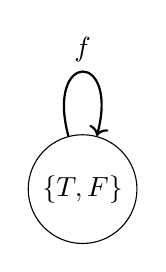
\begin{tikzpicture}
    % Define the node
    \node[circle, draw] (A) at (0,0) {$\{T,F\}$};
    
    % Draw self loop
    \draw[->, thick] (A) to[loop above] node[above] {$f$} (A);

\end{tikzpicture}
\end{center}

The above picture tells is that there \emph{is} a morphism called $f$, 
but it does not tell us anything about the \emph{content} of $f$. In particular, 
it is useful to know how $f$ maps elements of its domain to its codomain. 
To see this, we can draw the \textbf{internal picture} of this category
that visualizes the computational content of its morphisms:\footnote{Not 
all categories will have nice internal pictures, and different kinds of category 
will have their own visual language for describing their morphisms.}

\begin{center}
 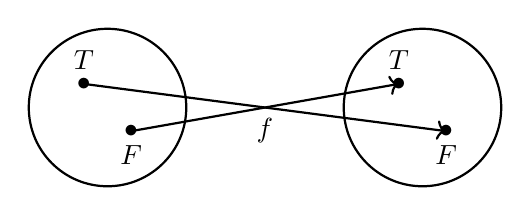
\begin{tikzpicture}
  % First circle with T and F dots
  \draw[thick] (0,0) circle (1);
  \node at (-0.3,0.3) {$\bullet$};
  \node at (-0.3,0.6) {$T$};
  \node at (0.3,-0.3) {$\bullet$};
  \node at (0.3,-0.6) {$F$};
  
  % Second circle with T and F dots
  \draw[thick] (4,0) circle (1);
  \node (T2) at (3.7,0.3) {$\bullet$};
  \node at (3.7,0.6) {$T$};
  \node (F2) at (4.3,-0.3) {$\bullet$};
  \node at (4.3,-0.6) {$F$};
  
    % Arrow from T on the left to F on the right
    \draw[->, thick] (-0.3,0.3) -- (4.3,-0.3);
    
    % Arrow from F on the left to T on the right
    \draw[->, thick] (0.3,-0.3) -- (3.7,0.3) node[midway, below] {$f$};
\end{tikzpicture}
\end{center}

Do not confuse the internal picture of a category with its picture: the internal 
picture ``peers inside objects'', and will not generalize to all kinds of categories.
This internal picture visualizes how the map $f$ behaves. A crucial 
piece information that this internal picture conveys is when two morphisms 
in \(\FinSet\) are equal: it is when they are \emph{extensionally equal}.

\todo: internal picture of \(\mathsf{not} \circ \mathsf{not} = \mathsf{id}\)


\section{Gaining intuition for categories}

The definition of category is highly abstract---and necessarily so, in order to be general enough
to accommodate all of the metalanguages just mentioned.
Next time, we will see how this level of abstraction allows for
clean axiomatizations of the various kinds of ``features'' that a metalanguage may support,
in the form of so-called ``universal constructions.''
This is what gives category theory its unifying power.

As preparation, we will first need to become quite comfortable working
with categories in the abstract. To do this, it is key to
have in mind a few representative examples of categories
to draw intuition from.

\subsection{Categories as graphs}

The first perspective on categories, which is perhaps most
comfortable to computer scientists, is that they are ``directed multigraphs with extra structure.''
Objects are vertices and morphisms are edges.
On top of this basic graph structure, categories come with a
composition operation that pastes two incident edges together to form a third,
and identity morphisms \(\mathsf{id}_A\) that form self-loops centered at each vertex \(A\).
The category laws then say that pasting of edges is an associative operation,
and that pasting with an identity morphism does nothing.
This provides nice visual intuition, and a large stock of example categories.
In fact,
\begin{construction}
  Every directed multigraph can be turned into a category.
\end{construction}
\begin{proof}
  Let \(G\) be a directed multigraph,
  encoded as a tuple \((V,E,\mathsf{src},\mathsf{trg})\)
  where \(V\) is the set of vertices, \(E\) is the set of edges,
  and \(\mathsf{src},\mathsf{trg}\) are functions \(E\to V\)
  that send each edge to its source and target vertices respectively.
  The graph \(G\) can be used to define a category
  \[
  \mathsf{paths}(G) = (O,M,\dom,\cod,\circ,\idt)
  \]
  where
  \begin{itemize}
  \item \(O = V\)
  \item \(M\) is the set of paths in \(G\),
    which are tuples \((v_s,[e_1,\dots,e_n],v_t)\)
    where \(v_s,v_t\) are vertices and \(e_1,\dots,e_n\) is a list of edges satisfying
    \(\mathsf{src}(e_1) = v_s\) and \(\mathsf{trg}(e_n) = v_t\)
    and \(\mathsf{trg}(e_i) = \mathsf{src}(e_{i+1})\)
    for all \(1\le i < n\).
  \item \(\dom : M \to O\) is the function \(\dom(v_s,[e_1,\dots,e_n],v_t) = v_s\)
  \item \(\cod : M \to O\) is the function \(\cod(v_s,[e_1,\dots,e_n],v_t) = v_t\)
  \item \(\circ\) concatenates paths:
    \((v_t,[f_1,\dots,f_n],v_u)\circ(v_s,[e_1,\dots,e_m],v_t) = (v_s,[e_1,\dots,e_m,f_1,\dots,f_n],v_u)\).
    Note that this is well-defined because the two paths \(\vec f\) and \(\vec e\) line up tip-to-tail.
    Note also that \(\vec e\) comes before \(\vec f\) in the concatenated path, due to the reversal of order
    of arguments to \(\circ\).
  \item \(\idt_v\) is the empty path \((v,[],v)\) starting and ending at \(v\).
  \end{itemize}
  The category laws are satisfied because concatenation of paths is associative and concatenating a path with the
  empty path does nothing.
\end{proof}
\begin{note}
  It is essential that morphisms are \emph{paths} in this construction, and not edges!
  Otherwise, it would be unclear how to define composition and identity.
\end{note}

\subsection{A Difference Between Categories and Directed Multigraphs}

A key difference between categories and graphs is that
two morphisms in a category that come from
different ``paths'' may nonetheless be equal.
For example, the following two ``paths'' through \(\FinSet\)
are actually the same, because negating a Boolean twice is the same as doing nothing:
\[% https://tikzcd.yichuanshen.de/#N4Igdg9gJgpgziAXAbVABwnAlgFyxMJZABgBpiBdUkANwEMAbAVxiRAB13gAVUgMU4BfEINLpMufIRQAmclVqMWbTj35CRYkBmx4CRAIykDC+s1aIOXXgPbDBCmFADm8IqABmAJwgBbJGQgOBBIRormKuy+dDgAFnAewJA49lrefqHUwUhy4cqWnNFxCUkQKZqePv6IgdmIuWb5VlhQOAD6wKo2QsLUDHQARjAMAAoSetIgXljOsTgiFIJAA
\begin{tikzcd}
{\{T,F\}} \arrow[rr, "\mathsf{not}"] \arrow[rd, "{\idt_{\{T,F\}}}"'] &           & {\{T,F\}} \arrow[ld, "\mathsf{not}"] \\
                                                                     & {\{T,F\}} &
\end{tikzcd}\]
This relationship between the paths \(\mathsf{not}\circ \mathsf{not}\) and \(\idt_{\{T,F\}}\)
is often conveyed by saying that the triangle above is ``filled in'', or ``commutes''.
The intuition being that one can then ``continuously deform''
\(\mathsf{not}\circ\mathsf{not}\) into \(\idt_{\{T,F\}}\),
by ``dragging'' it through the filled in triangle.

This idea is a handy visual tool for organizing categorical information
and for conducting proofs.

\subsection{Categories as orders}

A special case of a multigraph is a graph, where there is \emph{at most one} arrow between any given pair of vertices.
This leads us to the second class of important examples of a category:
\begin{definition}[preorder]
  \sloppy
  A preorder is a pair \((X,\preceq)\)
  where \(X\) is a set and \(\preceq\)
  is a binary relation on \(X\)
  that is reflexive (\(x\preceq x\) for all \(x\) in \(X\))
  and transitive (if \(x \preceq y\) and \(y\preceq z\) then \(x \preceq z\)).
\end{definition}
Preorders are often fruitfully drawn as \emph{Hasse diagrams}.
%% An object is like an element of a preorder
%% and a morphism \(x\to y\) is like a ``proof'' that \(x\le y\).
A simple example is the set \(\N\) of natural numbers,
ordered by \(m\preceq n\) if \(m\) is less than or equal to \(n\).
We can draw this preorder as follows:
\[
% https://tikzcd.yichuanshen.de/#N4Igdg9gJgpgziAXAbVABwnAlgFyxMJZABgBoBmAXVJADcBDAGwFcYkRiQBfU9TXfIRRkATNTpNW7AIzdeIDNjwEiZaeIYs2iECLl8lg1aWIbJ2kAB1LtKBBwIu4mFADm8IqABmAJwgBbJHIaHAgkERoACxh6KHZIMDYebz9AxAiQUKRpKJi4nQSk+V8A7JCwxDIQaNj4giTKLiA
\begin{tikzcd}
\vdots \arrow[d, no head] \\
2 \arrow[d, no head]      \\
1 \arrow[d, no head]      \\
0
\end{tikzcd}\]
Hasse diagrams are read bottom-up, with the least elements 
on the bottom and the greatest elements on the top. 
An undirected edge is drawn between elements with no elements 
between them (this is why we have no edge from 0 to 2 in the above figure).
A more visually interesting preorder on \(\N\)
is to define \(m \preceq n\) if \(m\) is a \emph{divisor} of \(n\).
This preorder looks less like a straight line and more like a lattice:
\[
% https://tikzcd.yichuanshen.de/#N4Igdg9gJgpgziAXAbVABwnAlgFyxMJZARgBoBmAXVJADcBDAGwFcYkRiQBfU9TXfIRQAGUgCZqdJq3ZjuvEBmx4CRMhJoMWbRCHLy+ywUTHjJWmboCsBxfxVDko4uek6QANltKBqlGRdNN3ZiYW97YxRTQKltEJseQ19HUWFXON0AHUzaKAgcBES7Iz9kUzSgjJBs3PzChR8HNVIK2MtqnLyC7kkYKABzeCJQADMAJwgAWyQyEBwIJFEQAAsYeih2SDA2IvGppFM5hcQl1fXNgh2FPenEchp5xZozjd0tq9GJ248H48OXi7bWw3JA-I5Ie4rNavcCXYFfJBWX4zZ7QwEfEAgxBI8F3VHnN5w3YIxAAFmRiH+aMJQOJ+zJFNmAJpGKx5NxAHZ8TD3vD6WDHogABzc9F8244wUATlFLJ6XCAA
\begin{tikzcd}
\vdots                                                      & \vdots                                                        & \vdots                                                       \\
6 \arrow[rd, no head] \arrow[d, no head] \arrow[u, no head] & 10 \arrow[ld, no head] \arrow[rd, no head] \arrow[u, no head] & 15 \arrow[ld, no head] \arrow[d, no head] \arrow[u, no head] \\
2 \arrow[rd, no head]                                       & 3 \arrow[d, no head]                                          & 5 \arrow[ld, no head]                                        \\
                                                            & 1                                                             &
\end{tikzcd}
\]
Preorders don't have to be discrete either: the real numbers \(\R\),
for instance, form a preorder with \(x \preceq y\) if \(x\) is less than or equal to \(y\). This is a little harder to draw.

A preorder that arises frequently in PL is the preorder of
\emph{run-time environments}.
It is common to model these environments
as partial functions \(\rho : \mathsf{Var} \rightharpoonup \mathsf{Val}\),
assigning to each program variable \(x \in \mathsf{Var}\)
a concrete value \(\rho(x)\).
These substitutions form a preorder, with \(\rho \preceq \rho'\)
if \(\rho\) is a subset of \(\rho'\), in the sense that all the 
variables in $\rho$ are in $\rho'$ and mapped to the same values.
%% \item Heaps under disjoint union: let \(\mathsf{Heap}\) be the category
%%   whose objects are substitutions \(\gamma\),
%%   i.e., partial functions \(\mathsf{Loc} \rightharpoonup \Z\),
%%   and whose morphisms from \(h\) to \(h'\)
%%   are heaps \(h_{\mathsf{diff}}\) such that \(h \uplus h_{\mathsf{diff}} = h\).

Preorders forms a category:
\begin{construction} \label{prop:every-preorder-is-a-category}
  Every preorder can be turned into a category.
  \label{eq:const-preorder}
\end{construction}
\begin{proof}
  For any preorder \((X,\preceq)\), there is a category
  \[
    \mathsf{order}(X,\preceq) = (O,M,\dom,\cod,\circ,\idt)
  \]
  where
  \begin{itemize}
    \item \(O = X\).
    \item \(M = (\preceq)\) (recall that a binary relation like \(\preceq\)
      can be thought of as a set of pairs, with \((x,y) \in (\preceq)\)
      if and only if \(x\preceq y\)).
    \item \(\dom\) is the function \(\dom(x,y) = x\).
    \item \(\cod\) is the function \(\cod(x,y) = y\).
    \item \(\circ\) is the function defined by \((y,z)\circ(x,y) = (x,z)\).
      Note that we may assume that the two arguments to \(\circ\)
      share a component \(y\) in this definition because of the assumption
      that \((y,z)\) and \((x,y)\) are composable.
      Note also that the composite \((x,z)\) is indeed well-defined
      this is well defined by the transitivity of \(\preceq\).
    \item \(\idt_x\) is the pair \((x,x)\), which forms a valid morphpism
      by reflexivity of \(\preceq\).
  \end{itemize}
  The category laws are satisfied automatically,
  as there can only be at most one morphism between any two objects.\footnote{Pause: 
  why is this the case?}
\end{proof}
\noindent
The intuitive import of Proposition~\ref{prop:every-preorder-is-a-category}
is that every category can be thought of as a kind of preorder,\footnote{\emph{Reminder}: not all 
categories directly correspond to some preorder construction, since there can be multiple 
morphisms between objects in a general category. A category with at most 1 morphism between 
any 2 objects is called a \emph{thin category}, and it does correspond to some preorder.}
where the existence of a morphism \(A\xrightarrow{f} B\)
expresses that \(A\) is in some sense ``less than or equal to'' \(B\).
Thinking of categories in this way leads to interesting questions like:
\begin{itemize}
\item
  Does a category have a ``smallest'' or ``largest'' object?
  For instance, the smallest runtime environment is the empty environment $\emptyset$
  with no variables in it.
\item Does a category have ``ascending sequences''?
  For example, 
  \begin{align}
   \emptyset \subseteq \{x\mapsto A\} \subseteq \{x\mapsto A, y\mapsto B\} \subseteq \dots 
   \label{eq:env-seq}
  \end{align}
  is an ascending sequence in the preorder of runtime environments.
\item  Does a category have ``limit'' objects, like suprema or infima?  For
  instance, you probably know from calculus that there limits in \(\R\): for
  example, the sequence $\frac{1}{2}, \frac{1}{4}, \frac{1}{8},
  \frac{1}{16}\cdots$ approaches 0 in the limit.  A very interesting question is:
  which categories ``have limits'', in the sense that such sequences always
  converge to some object in the category?

  An example of a situation where there is no limit is the sequence in
  \cref{eq:env-seq}.  The set of environments grows and grows, and since there
  is no notion of a ``greatest environment'', there is no limit to this
  sequence.
\item
  Given two categories, is there a notion of ``monotone map'' between them?
\end{itemize}

Each of the above observations is foreshadowing a notion of a ``universal construction''
in a category, which we will explore in the following lectures.

\subsection{Categories as algebras}

Whereas preorders are like multigraphs where there is at most one \emph{edge}
between any two vertices,
the opposite extreme is a multigraph with exactly one \emph{vertex},
so that all edges are self-loops:
% https://q.uiver.app/#q=WzAsMSxbMCwwLCJcXGJ1bGxldCJdLFswLDBdLFswLDAsIiIsMCx7InJhZGl1cyI6MX1dLFswLDAsIiIsMCx7InJhZGl1cyI6NX1dXQ==
\begin{equation}
\begin{aligned}
\begin{tikzcd}
	\star
	\arrow[from=1-1, to=1-1, loop, in=55, out=125, distance=10mm]
	\arrow[from=1-1, to=1-1, loop, in=60, out=120, distance=5mm]
	\arrow[from=1-1, to=1-1, loop, in=50, out=130, distance=15mm]
\end{tikzcd}
\end{aligned}
\end{equation}
Categories of this shape form our final class of important example:
a special kind of algebraic structure called a \emph{monoid}.
\begin{definition}[monoid]
  A monoid is a tuple \((X,\bullet,e)\)
  where \(\bullet\) is a binary operation on \(X\)
  (a function \(X \times X \to X\))
  that is associative (\(x\bullet (y\bullet z) = (x\bullet y) \bullet z\))
  and has \(e\) as a unit (\(x\bullet e = x\) and \(e\bullet x = x\)).
\end{definition}
A simple example of a monoid is \((\N,+,0)\),
the monoid of natural numbers under addition.
This forms a monoid because addition of natural numbers is associative
and has zero as a unit.

An example that is closer to PL
comes from the semantics of imperative programs.
It is common to interpret an imperative program
as a function \(S \to S\), where \(S\) is a set of
memory states.
For example, the program
\[
  x := x + 1;
\]
can be interpreted
as a function that sends a memory state \(s\)
to a new memory state \(s'\) in which
the value of \(x\) has been incremented by \(1\).
The functions \(S \to S\) form a monoid
\((S\to S,\bullet,\mathsf{id})\),
where the monoid operation is given by \(f \bullet g = g \circ f\)
(note the reversal!),
corresponding to the sequencing of the programs \(f\) and \(g\),
and the identity element is the identity function on \(S\),
corresponding to the empty program that does nothing.

Algebraic identities capture program rewrites for this imperative language.
For example, if \(f\) is the interpretation of \(x := 0\)
and \(g\) is the interpretation of \(y := 1\),
and \(x\) and \(y\) are distinct program variables,
then the program equation
\begin{equation}
  \left(\begin{aligned}
    &x := 0 \\
    &y := 1
  \end{aligned}\right)
  \equiv
  \left(\begin{aligned}
    &y := 1 \\
    &x := 0
  \end{aligned}\right)
\end{equation}
can be expressed as the algebraic identity \(g \circ f = f \circ g\).

\begin{construction} \label{prop:every-monoid-is-a-category}
  Every monoid can be turned into a category.
\end{construction}
\begin{proof}
  For any monoid \((X,\bullet,e)\) there is a category
  \[
    \mathsf{mon}(X,\bullet,e) = (O,M,\dom,\cod,\circ,\idt)
  \]
  where
  \begin{itemize}
  \item \(O = \{\star\}\), a singleton set with a single dedicated element \(\star\).
    \marginnote{Technically set theory does not contain stars in it.
    But this is no matter.
    The symbol \(\star\) can be interpreted as any object of
    your choice---all that matters
    is that \(O\) is a singleton set.
    For instance, one could set \(\star =
    \varnothing\).
    }
  \item \(M = X\)
  \item \(\dom(M) = \star\)
  \item \(\cod(M) = \star\)
  \item Composition is defined by \(x \circ y = x \bullet y\)
  \item \(\idt_\star = e\)
  \end{itemize}
  The category laws follow from the associativity of \((\bullet)\)
  and that it has \(e\) as a unit.
\end{proof}
\begin{note}
  It is very important that the set of objects \(O\) is a singleton set \(\{\star\}\).
  A natural thought one might have is that the set of objects should be the set \(X\) of elements of the monoid.
  But this in fact does not work: what would be the morphisms?

  There is actually a good reason why the set of objects is the seemingly-arbitrary singleton set \(\{\star\}\) in this construction.
  It comes from the fact that a monoid is what is called a \emph{single-sorted} algebraic structure; hence \(\{\star\}\)
  is a set with a single element.
\end{note}
The intuitive import of
Proposition~\ref{prop:every-monoid-is-a-category} is that
every category can be thought of as a kind of algebraic structure,
where composition is like ``multiplication''
and identity morphisms are like ``multiplicative units''.

The algebraic perspective leads to questions like:
given an equation between morphisms containing some unknowns,
are there zero, one, or infinitely many solutions?
When can I ``cancel'' a morphism from both sides of an equation (e.g., from \(fg = fh\) deduce \(g=h\),
or from \(fh = gh\) deduce \(f=g\))?
When does a morphism have an ``inverse''?
When can a morphism \(f\) be ``factored'' into two pieces, \(f = gh\)?


\section{Putting intuitions to the test}

We conclude this section by illustrating each of the three perspectives
on categories on the following
\textbf{categorification}\footnote{The idea of ``categorification'' is to 
cast a notion one is familiar with -- like ``subset inclusion'' into 
the language of objects and morphisms. This is a very important idea 
in category theory because it allows one to take familiar concepts 
and apply them to unfamiliar categories.} of
a basic concept from set theory: subset inclusion.
\begin{proposition} \label{prop:subset-leq-iff-triangle}
Suppose \(U\) and \(V\) are subsets of a finite set \(X\).
Then \(U \subseteq V\) if and only if
there exists a dashed \(\FinSet\)-morphism \(f\)
such that \(v \circ f = u\),
where \(u\) and \(v\) are the \(\FinSet\)-morphisms
corresponding to the inclusion functions\footnote{A function $f : X \to Y$ 
is an \emph{inclusion function} (also called an ``injective map'') if 
each element of $X$ is mapped to a unique element in $Y$. 
All inclusion functions have a ``left inverse'': 
there exists a function $g$ such that $g \circ f = \mathsf{id}_X$.
Inclusion maps are rendered using tailed arrows.} \(U \to X\) and \(V \to X\)
respectively:
\begin{equation}
  % https://tikzcd.yichuanshen.de/#N4Igdg9gJgpgziAXAbVABwnAlgFyxMJZABgBpiBdUkANwEMAbAVxiRAFUQBfU9TXfIRQAmclVqMWbAGrdeIDNjwEiARlKrx9Zq0QgAGt3EwoAc3hFQAMwBOEALZIyIHBCSiXdLAzY4vP6m0pPSYQagY6ACMYBgAFfmUhEBssUwALHDlrO0dEdRc3RA8-b19-MIkdNhoskFsHJ2pXJHySnz1IMFZwrC62KDo4NJMKoN06oy4gA
\begin{tikzcd}
U \arrow[rd, "u"', tail] \arrow[rr, "f", dashed] &   & V \arrow[ld, "v", tail] \\
                                                 & X &
\end{tikzcd}
\end{equation}
\end{proposition}
You will prove Proposition~\ref{prop:subset-leq-iff-triangle} in the homework.
As preparation,
let's appreciate what it is saying: a basic set theoretic
property \(U\subseteq V\) about finite subsets
can be recast in terms of a purely category-theoretic property
about \(\FinSet\).
This categorification takes roughly two steps.
The first step is to express the subsets \(U\) and \(V\)
as morphisms \(u\) and \(v\).
The second step is to express \(U\subseteq V\)
as a property of the morphisms \(u\) and \(v\).
Let's try to get some intuition for what this property is saying
from each of the perspectives we've developed so far.
\begin{itemize}
\item Graphically, it says that the morphisms \(u\) and \(v\)
  fit into a triangle with \(f\) that is ``filled in''.
\item Order-theoretically, it says that the morphism \(u\) is somehow
  ``less than or equal to'' \(v\), by virtue of there being a dashed morphism
  \(f\) witnessing this order relationship.

  We can make this formal as follows.
  For any finite set \(X\), one can construct a category \(\mathsf{Sub}(X)\).
  The objects of this category are tuples \((U,u)\) where \(U\) is a subset of \(X\)
  and \(u\) is the function \(U \to X\) defined by \(u(x) = x\);
  i.e., \(u\) is the canonical inclusion function of \(U\) into \(X\).
  The morphisms of this category are, roughly speaking,
  pictures of the following shape:
  \[
  % https://tikzcd.yichuanshen.de/#N4Igdg9gJgpgziAXAbVABwnAlgFyxMJZABgBpiBdUkANwEMAbAVxiRAFUQBfU9TXfIRQBGUsKq1GLNgA1uvEBmx4CRAEzkJ9Zq0QgAatwkwoAc3hFQAMwBOEALZIyIHBCSjJOtkxDUGdACMYBgAFfhUhEBssUwALHHlrO0dEDRc3RA9taT0aRJBbBydqVyQ07N0Coy4gA
\begin{tikzcd}
U \arrow[rd, "u"'] \arrow[rr, "f"] &   & V \arrow[ld, "v"] \\
                                   & X &
\end{tikzcd}
  \]
  Formally, a morphism is a tuple \((U,u,f,V,v)\)
  where \(U\) and \(V\) are subsets of \(X\),
  \(u : U \to X\) and \(v : V \to X\) are the canonical inclusions,
  and \(f\) is a function \(U \to V\)
  such that \(v \circ f = u\).
  Each morphism \((U,u,f,V,v)\) has domain \((U,u)\)
  and codomain \((V,v)\).

  Now Proposition~\ref{prop:subset-leq-iff-triangle}
  says that \(U\subseteq V\) if and only if there is a morphism from \((U,u)\)
  to \((V,v)\) in the category \(\mathsf{Sub}(X)\),
  witnessing the fact that \((U,u)\) is ``less than or equal to'' \((V,v)\).

\item Algebraically, it says that the equation \(u = v \circ f\)
  has a solution in the unknown \(f\).
\end{itemize}
Let's see each of these in action on the following proof.
\begin{proposition}
  If \(U\subseteq V\) and \(V \subseteq W\) then \(U\subseteq W\).
\end{proposition}
Each perspective lends itself to a different proof strategy.
\begin{itemize}
\item Graphically, you paste two filled in triangles to get a bigger filled in triangle.
\item Order-theoretically, you use the fact that \(\mathsf{Sub}(X)\), as a category,
  has composition.
\item Algebraically, you use that \(u = vf = wvg\) provides a solution to \(u = wh\).
\end{itemize}

%% \item Refinement corresponds to solvability of an equation that looks like a square.
%%   Suppose you have a subset \(U\) of a finite set \(X\),
%%   a subset \(V\) of a finite set \(Y\),
%%   and a function \(f : X \to Y\).
%%   Let \(u : U \rightarrowtail X\) and \(v : V \rightarrowtail Y\) be the relevant inclusions.

%%   Suppose \(f\) satisfies the property that,
%%   for all \(x \in U\), it holds that \(f(x) \in V\).
%%   This can be expressed as saying that the equation
%%   \(fu = vg\) is \emph{solvable} in the unknown \(g\).
%%   Diagramatically:
%%   \[
%%   % https://tikzcd.yichuanshen.de/#N4Igdg9gJgpgziAXAbVABwnAlgFyxMJZABgBpiBdUkANwEMAbAVxiRAFUQBfU9TXfIRQBGclVqMWbAGrdeIDNjwEiZYePrNWiEAA05fJYKKj11TVJ0BNbuJhQA5vCKgAZgCcIAWyRkQOCCQAJmocOiwGNjCIkHNJbRAmWJAGOgAjGAYABX5lIRB3LAcACxwDEA9vJFF-QMQAZlDwyJ1oyLitNhpyyp9EPwDqjssQBx7PPpDapEaJTp1XZNSM7NzjHUKSsq4KLiA
%% \begin{tikzcd}
%% U \arrow[d, "u"', tail] \arrow[r, "g"] & V \arrow[d, "v", tail] \\
%% X \arrow[r, "f"']                      & Y
%% \end{tikzcd}
%%   \]
%%   This situation actually comes up quite a lot in PL,
%%   as we will see when we discuss logical relations.

%%   (By the way, the solution \(g\), if it exists, must be the \emph{only} solution to this equation,
%%   as if one finds \(g\) and \(g'\) such that \(fu = vg\) and \(fu = vg'\), then \(vg=fu=vg'\),
%%   and left-cancellativity of \(v\) implies \(g = g'\).)

\subsection{Some fun exercises}

\begin{itemize}
\item Explicitly write down the monoid \((\N,+,0)\) as a category.
\item Solve the equation \(c \circ (x := x + 1) = (x := x + 2)\) for \(c\).
  Can you find any other solutions?
\item Try to come up with an English description of what it means for an Imp command to be ``left'' or ``right'' cancellable
\item Prove Proposition~\ref{prop:subset-leq-iff-triangle}.
\item Show that the functions \(u,v\) in Proposition~\ref{prop:subset-leq-iff-triangle}
  are left-cancellable as morphisms of \(\FinSet\).
\end{itemize}

\chapter{Universal Constructions I}
We've been hinting at the utility of knowing that categories that have certain
special objects in them. For example, if we want to give a category that lets us
validate equations of programming languages, that category will need to be able 
to represent the many features that programs might have: products, sums, 
functions, etc. Here we will introduce the essential idea of a \textbf{universal 
construction} that characterizes when categories contain these special objects.

\section{Terminal objects \& the unit type}
Recall that when designing categorical semantics for programming languages we
associate types and typing contexts with objects in the category and terms with
morphisms. Concretely, if we have a well-typed term $\Gamma \vdash e : A$,
its interpretation $\dbracket{\Gamma \vdash e : A}$ is a morphism
$\dbracket{\Gamma} \xrightarrow{\dbracket{e}} \dbracket{A}$.
Previously, we showed how \(\FinSet\) can be used to give an interpretation 
to \ref{lang:calc} programs by associating types like the unit type $\plUnit$
with special sets, like a set containing only a single element $\{\star\}$.
But, what if we want to see if categories other than $\FinSet$ can give give a 
reasonable interpretation for $\plUnit$?

To proceed, let's pick a particular object $\dbracket{\plUnit}$ 
in a category $\calC$ and explore what properties it needs to have in order 
to be ``$\plUnit$-like'':
\begin{itemize}
  \item \textbf{Fact 1, Introduction rules}: It must be possible in any typing context to
  produce a value of type $\plUnit$.  This tells us that for any context
  $\Gamma$, there must exist a $\calC$-morphism
  $\dbracket{\Gamma} \to \dbracket{\plUnit}$.
  For example, it must 
  be the case that 
  $\dbracket{\Gamma} \xrightarrow{\dbracket{\plunit}} \dbracket{\plUnit}$.

  \item \textbf{Fact 2, Equational laws}: Since \ref{lang:calc} has no effects, 
  it is the case that if $\Gamma \vdash e : \plUnit$, then it is indistinguishable 
  from the term $\plunit$. This is called \textbf{eta equality}, and we write
  this as $e \equiv \plunit$.\footnote{The symbol ``$\equiv$'' means ``is
  equationally equal to''.} Eta equality is an equational law that characterizes
  how a $\plUnit$ term must behave. Now for an insight: \emph{these equational
  laws are translated into morphism equalities}. It must be that, for any
  morphism $\dbracket{\Gamma} \xrightarrow{\dbracket{e}} \dbracket{\plUnit}$, it
  is the case that $\dbracket{e} = \dbracket{\plunit}$.  In other words, the
  morphism $\dbracket{\Gamma} \xrightarrow{\dbracket{\plunit}} \plUnit$ must be
  unique.
\end{itemize}

These two properties can be packaged up into a nice concise definition:

\begin{definition}[Terminal object]  \label{def:terminal-object}
  Let $T$ be an object in a category $\calC$. 
  An object $T$ in $\calC$ is called a terminal object
  if
  \begin{itemize}
  \item
    for every object \(\Gamma\) in \(\calC\)
    there is a morphism \(\Gamma \xrightarrow{\angled{}} T\);
  \item
    for every morphism \(\Gamma \xrightarrow{f} T\)
    it holds that \(f = \angled{}\).
  \end{itemize}
\end{definition}

Let's pause to remark on the three categorical interpretations 
of terminal objects $T$:
\begin{itemize}
  \item Graphically, an object is terminal if (1) there is an arrow from 
  every other object to it, and (2) it ``thins all parallel
  arrows'', meaning that if we have a situation like the following for 
  and morphisms $X \xrightarrow{f} T, X \xrightarrow{g} T$:
  \begin{align*}
    % https://tikzcd.yichuanshen.de/#N4Igdg9gJgpgziAXAbVABwnAlgFyxMJZABgBpiBdUkANwEMAbAVxiRABUQBfU9TXfIRRkAjFVqMWbABrdxMKAHN4RUADMAThAC2SEdRwQkZEACMYYKEgC0AZhMM65hgAV+eAmw1ZFACxwg1PTMrIggity8IJo6egZGiCbmlkj21I7ObtgeQiAMMGoBQZKh0XJcQA
\begin{tikzcd}
  T                                                       \\
  X \arrow[u, "g"', bend right] \arrow[u, "f", bend left]
  \end{tikzcd},
  \end{align*}
  then we know that $f = g$.
  In other words, there is a unique morphism \(\Gamma \to T\) for every \(\Gamma\):
  \begin{center}
% https://tikzcd.yichuanshen.de/#N4Igdg9gJgpgziAXAbVABwnAlgFyxMJZABgBpiBdUkANwEMAbAVxiRAEEQBfU9TXfIRQBGclVqMWbACrdxMKAHN4RUADMAThAC2SMiBwQkokAyxhWiEHAhmoIagzoAjGAwAK-PATYMYanAcJZksQAB0wmAAPLDgcOABCOS4gA
\begin{tikzcd}
  A \arrow[r, "\exists!"] & T
  \end{tikzcd}
\end{center}
  \item The order-theoretic perspective is that the terminal object 
  is the ``greatest object'' in the category.
  \item The algebraic perspective
    says that, for every object \(\Gamma\),
    the equation \(f = f\) has a unique solution
    in the unknown \( \Gamma \xrightarrow{f} T\).
\end{itemize}

We say a category \textbf{has terminal objects} if there is an object in the
category that is a terminal object. This is our first example of a 
\textbf{universal construction}, which are special objects in categories 
characterized by their morphisms into them. We will see how universal 
constructions can be used to give interpretations to all the type 
formers we have seen so far. But, we can already see their utility: 
whether or not a particular category admits certain universal constructions
will immediately inform us of that category's suitability for modeling 
certain language properties.

\subsection{$\FinSet$ has terminal objects, isomorphisms}
We saw in previous lectures that we could use the singleton set 
$\{\star\}$ to give an interpretation to $\plUnit$ in $\FinSet$.
We can easily prove that $\{\star\}$ is a terminal object:
\begin{theorem}
  The singleton set $\{\star\}$ is terminal in $\FinSet$.
\end{theorem}
\begin{proof}
  \begin{itemize}
    \item Existence: The map $\_ \mapsto \{\star\}$ has the required type.
    \item Uniqueness: Suppose we have two morphisms $A \xrightarrow{f} \{\star\}$ and
    $A \xrightarrow{g} \{\star\}$. 
    Then by function extensionality we immediately have that $f = g$ 
    as set-functions, and so they are equal as $\FinSet$ morphisms.
  \end{itemize}
\end{proof}

Now you can observe the above proof and see that it immediately 
works for \emph{any} choice of singleton set: does this mean that $\FinSet$
has \emph{many terminal objects?} Yes, and no. \emph{Yes}, in the sense 
that there are indeed many valid choices of terminal object; but \emph{no}, 
in the sense that the choice itself does not (\emph{should} not!) actually 
matter. We capture this by the notion of isomorphism:

\begin{definition}[Isomorphism of objects]
  \sloppy
  Two objects $A$ and $B$ in a category $\calC$ are isomorphic if 
  there exist morphisms $A \xrightarrow{f} B$ and $B \xrightarrow{g} A$
  such that (1) $g \circ f = \id_A$ and (2) $f \circ g = \id_B$.
\end{definition}

We can immediately see that any two singleton sets in $\FinSet$ are isomorphic:
this proof is straightforward. What might be surprising is that this 
fact is true for all terminal objects:

\begin{theorem} \label{thm:terminal-object-unique}
  Terminal objects are unique up to isomorphism.
\end{theorem}
\begin{proof}
  Let $X$ and $Y$ be terminal objects in some category $\calC$. 
  Then there exists a pair of unique morphisms between them:

  \begin{center}
 % https://tikzcd.yichuanshen.de/#N4Igdg9gJgpgziAXAbVABwnAlgFyxMJZABgBpiBdUkANwEMAbAVxiRAA0QBfU9TXfIRQBGclVqMWbAJrdxMKAHN4RUADMAThAC2SMiBwQkokACMYYKEgDM++s1aIQAQjXdeITTuPVDe6uaWNnaSji6KclxAA
\begin{tikzcd}
  X \arrow[r, "!f", bend left] & Y \arrow[l, "!g", bend left]
  \end{tikzcd} 
\end{center}
By the fact that $X$ and $Y$ are terminal, they must also have unique identity
morphisms $\id_X$ and $\id_Y$. Then by the uniqueness of identity we have that $g \circ f = \id_X$ and $f \circ g = \id_Y$.
\end{proof}

This provides some evidence that the choice of terminal object does not matter.
  But are we done? Suppose we had two terminal objects \(T\) and \(T'\).
  By the above argument, we have that these two objects are isomorphic.
  But now another potential choice arises: what if there are multiple different
  \emph{isomorphisms} between \(T\) and \(T'\)?
  Then it could be that the choice to use \(T\) instead of \(T'\)
  may implicitly come with a choice of specific isomorphism as well.

  Luckily, terminal objects satisfy a stronger property
  which ensures that one's choice is terminal object is truly irrelevant.

\begin{proposition}
  Terminal objects are unique up to \emph{unique} isomorphism.
  That is, if \(T\) and \(T'\) are both terminal,
  then there is exactly one isomorphism
  \((f:T\to T',g:T'\to T)\)
  between \(T\) and \(T'\).
\end{proposition}
\begin{proof}
  Both \(f\) and \(g\), as constructed in the proof of
  \Cref{thm:terminal-object-unique},
  are the only possible morphisms \(T \to T'\) and \(T'\to T\)
  respectively. Thus they together form the only isomorphism
  between \(T\) and \(T'\).
\end{proof}

Later on, when we have the language for it, we will show that
all universal constructions are unique up to unique isomorphism
in this sense, and hence free of non-canonical choices.


% \subsection{Terminal objects for preorders}
% Universal constructions are one of the engines for analogy in category theory:
% very different-seeming concepts can be cast as instances of the same 
% universal construction, which can bring clarity to what each of those disparate 
% concepts means. When cast order-theoretically, the terminal object can 
% be thought of as ``the greatest object in a category.''
% % The first instance we will see of a universal construction is a \textbf{terminal 
% % object}, which can be thought of as ``the largest object in a category'' if one 
% % recalls the preorder intuition of morphisms. 

% An element of a preorder is the largest if it is greater than every other 
% element: i.e., there exists a morphism from every other element to it.
% This definition works for a general category: one could say an object is 
% largest if there exists a morphism from every other object into it.
% This characterization however doesn't take into account that there 
% can be more than 1 morphism between any two objects in a category: intuitively, 
% this means that one object can be greater than another in more than one way.

\section{Products}
Next we want to interpret product types $A \times B$. As before with the 
unit type, the typing rules for products forces the existence of certain morphisms,
and the equational theory of products forces equalities of certain morphisms.
The  introduction rule that describes how to create new products is:
\begin{mathpar}
\inferrule
    {\Gamma\vdash M : A
      \\
    \Gamma\vdash N : B
    }
    {\Gamma \vdash \plpair{M}{N} : A \pltimes B}~(\textsc{T-Pair})
\end{mathpar}
The elimination rules that break apart products are:
\begin{mathpar}
\inferrule
    {\Gamma\vdash M : A \pltimes B}
    {\Gamma \vdash \plfst{M} : A}~(\textsc{T-Fst})
\and
\inferrule
    {\Gamma\vdash M : A \pltimes B}
    {\Gamma \vdash \plsnd{M} : B}~(\textsc{T-Snd})
\end{mathpar}

These rules imply the existence of several morphisms that characterize 
what it means for for a special object $\dbracket{A \times B}$ to be a 
product. Reading off from the rules:
\begin{itemize}
  \item The \textsc{T-Pair} rules says that if there are 
  two morphisms $\dbracket{\Gamma} \mor{\dbracket{M}} \dbracket{A}$ and 
  $\dbracket{\Gamma} \mor{\dbracket{N}} \dbracket{B}$, 
  then there is a morphism $\dbracket{\Gamma} \mor{\dbracket{\langle M, N \rangle}} 
  \dbracket{A \times B}$.
  \item The \textsc{T-Fst} rule says that if there is a morphism 
  $\dbracket{\Gamma} \mor{\dbracket{M}} 
  \dbracket{A \times B}$, then there is a 
  morphism $\dbracket{\Gamma} \mor{\dbracket{\plfst{-}}} \dbracket{A}$.\footnote{Note:
  We are naming these morphisms \emph{suggestively}. The typing rules only enforce 
  the \emph{existence} of certain morphisms: they don't tell us anything about 
  how they behave.}
  \item The \textsc{T-Snd} rule says that if there is a morphism 
  $\dbracket{\Gamma} \mor{\dbracket{M}} 
  \dbracket{A \times B}$, then there is a 
  morphism $\dbracket{\Gamma} \mor{\dbracket{\plsnd{-}}} \dbracket{B}$.
\end{itemize}

We can package these morphisms up into the following diagram:

\begin{equation}
 % https://tikzcd.yichuanshen.de/#N4Igdg9gJgpgziAXAbVABwnAlgFyxMJZARgBoAGAXVJADcBDAGwFcYkQAdDgcXoFs+9EAF9S6TLnyEUZYtTpNW7AIIACLnj7xVAIRFiQGbHgJFypAEzyGLNohDL9441KIXL1xXZB7h8mFAA5vBEoABmAE4QfEjmIDgQSGQKtuxcjPRggYwwqgCypKoAclwRmdm5TiCR0Uk0CUjuIBkARjCMAAoSJtIgEViBABY4IDQ2SvZhcCOi4VExiMkNiADMNK3tXS6m9jlhI2Ne7HBgUFU1C3HLTW2nSAC0K3Hj3nnn87H1ias0t2erzyO9iKIkowiAA
\begin{tikzcd}[column sep = huge]
  & \dbracket{\Gamma} \arrow[d, "{\dbracket{\langle M, N\rangle }}"] \arrow[ldd, "\dbracket{M}" description, bend right] \arrow[rdd, "\dbracket{N}" description, bend left] &   \\
  & \dbracket{A \times B} \arrow[ld, "\dbracket{\plfst{-}}"' description] \arrow[rd, "\dbracket{\plsnd{-}}" description]                                                     &   \\
\dbracket{A} &                                                                                                     & \dbracket{B}
\end{tikzcd}
\label{cd:prod1}
\end{equation}

Next, the equational theory of products will assert certain equalities of
morphisms. We begin with the \emph{$\beta$-rules} that give the equational 
behavior of elimination after introduction:
% (elim after intros sometimes called \(\beta\) rules)
\begin{mathpar}
\inferrule
    {\Gamma\vdash M : A
      \\
    \Gamma\vdash N : B
    }
    {\Gamma \vdash \plfst{\plpair{M}{N}} \equiv M : A}~(\beta^{\pltimes}_1)
\and
\inferrule
    {\Gamma\vdash M : A
      \\
    \Gamma\vdash N : B
    }
    {\Gamma \vdash \plsnd{\plpair{M}{N}} \equiv N : B}~(\beta^{\pltimes}_2)
\end{mathpar}
Translating these equations into morphism equalities:
\begin{itemize}
  \item $\beta_1$ enforces that $\dbracket{M} = 
  \dbracket{\plfst{-}} \circ \dbracket{\langle M, N \rangle}$ 
  in (\ref{cd:prod1})
  \item $\beta_2$ enforces that $\dbracket{N} = 
  \dbracket{\plsnd{-}} \circ \dbracket{\langle M, N \rangle}$ 
  in (\ref{cd:prod1})
\end{itemize}

Hence, the $\beta$-rules together enforce that the diagram in \ref{cd:prod1} commutes.
Next, we consider the second part of the equational theory of products
that describes the behavior of introduction after elimination, sometimes called the \emph{\(\eta\)-rules}:
\begin{mathpar}
\inferrule
    {\Gamma\vdash M : A \pltimes B
    }
    {\Gamma \vdash M \equiv \plpair{\plfst{M}}{\plsnd{M}} : A \pltimes B}~(\eta^{\pltimes})
\end{mathpar}

This law says asserts the extensional equality of any two pair-formation
operations.  Translated into morphisms, it says that any morphism of the form
$\dbracket{\Gamma} \mor{\dbracket{M}} \dbracket{A \times B}$ is is equal to a
canonical morphism $\dbracket{\Gamma} \mor{\dbracket{\langle \plfst{M},
\plsnd{M} \rangle}} \dbracket{A \times B}$.  Put another way: there is a unique
morphism $\dbracket{\Gamma} \mor{} \dbracket{A \times B}$ making the above diagram \textbf{commute}.\footnote{Formally,
a diagram \textbf{commutes} if every face of the diagram is ``filled in'', 
meaning that all paths beginning and ending in the same place are equal 
as morphisms.}

\subsection{Packaging up intuition into a definition}
Now, as in the case of terminal objects, we can give a more generic description of 
products that isn't so specific to the case of equational theories of programs:

\begin{definition}[Product] \label{def:product}
  Let \(A\) and \(B\) be two objects of a category \(\calC\).
  A \emph{product of \(A\) and \(B\)}
  is a tuple \((P,\pi_A,\pi_B)\)
  where
  \begin{itemize}
  \item \(P\) is an object of \(\calC\).
  \item \(\pi_A\) is a morphism from \(P\) to \(A\),
    called the \emph{projection onto \(A\)}.
  \item \(\pi_B\) is a morphism from \(P\) to \(B\),
    called the \emph{projection onto \(B\)}.
  \end{itemize}
  such that
  \begin{itemize}
  \item For any object \(\Gamma\) and any two morphisms \(f : \Gamma \to A\)
    and \(g : \Gamma \to B\),
    there exists a morphism \(\angled{f,g} : \Gamma \to P\)
    such that the following equations hold:
    \begin{align}
      \pi_A \circ \angled{f,g} = f \\
      \pi_B \circ \angled{f,g} = g
    \end{align}
  \item The following equation holds for any morphism \(h : \Gamma \to P\).
    \begin{align}
      h = \angled{\pi_A \circ h, \pi_B \circ h}
    \end{align}
  \end{itemize}
\end{definition}

\begin{proposition}
  Let \(A\) and \(B\) be finite sets.
  The tuple \((A \times B, \pi_A, \pi_B)\)
  is a product in \(\FinSet\),
  where \(\pi_A\) is the morphism \((A\times B,\pi_A, A)\)
  and \(\pi_B\) is the morphism \((A \times B,\pi_B,B)\).
\end{proposition}

\begin{proposition}
  Let \(A\) and \(B\) be two objects of a category \(\calC\).
  A tuple \((P,\pi_A,\pi_B)\) is a product of \(A\) and \(B\)
  if and only if the following \textbf{universal property}
  holds:
  for any object \(\Gamma\) and any two morphisms \(f : \Gamma \to A\)
  and \(g : \Gamma \to B\),
  there exists a unique morphism \(h : \Gamma \to P\)
  such that \(\pi_A \circ h = f\) and \(\pi_B \circ h = g\).
\end{proposition}
\begin{proof}
  Suppose \((P,\pi_A,\pi_B)\) is a product of \(A\) and \(B\).
  By definition of product, we have for any \(\Gamma\) and morphisms \(f : \Gamma \to A\)
  and \(g : \Gamma \to B\)
  that the morphism \(\angled{f,g} : \Gamma \to P\)
  satisfies \(\pi_A \circ \angled{f,g} = f\)
  and \(\pi_A \circ \angled{f,g} = g\).
  This morphism is the unique such, because
  if any morphism \(h : \Gamma \to P\)
  satisfies \(\pi_A \circ h = f\) and \(\pi_B \circ h = g\)
  then it must be that
  \begin{equation}
    h = \angled{\pi_A \circ h, \pi_B \circ h} = \angled{f,g}.
  \end{equation}
  Conversely, if \((P,\pi_A,\pi_B)\) is any tuple satisfying
  the above universal property,
  then one can define \(\angled{-,-}\)
  as the function that sends each pair of morphisms \(f : \Gamma \to A\)
  and \(g : \Gamma\to B\)
to the unique \(h\) such that \(\pi_A \circ h = f\) and \(\pi_A \circ h = g\).
\end{proof}

Algebraically, the universal property can be formulated as saying
  the following system of equations has exactly one solution
  in the unknown \(h : \Gamma \to P\).
  \begin{align}
    \pi_A \circ h = f \\
    \pi_B \circ h = g
  \end{align}
Diagramatically, it can be formulated as saying there exists a unique
dashed arrow that fills in all the triangles in the following picture.
\begin{equation}
% https://tikzcd.yichuanshen.de/#N4Igdg9gJgpgziAXAbVABwnAlgFyxMJZABgBoBGAXVJADcBDAGwFcYkQAdDgcXoFs+9EAF9S6TLnyEU5CtTpNW7AAoixIDNjwEiAJlLF5DFm0QgAgmvFape0rqOLTIAEIj5MKAHN4RUADMAJwg+JDIQHAgkfQUTdn8QGgAjGDAoJABmYlEA4NDEcMikWRBGLDBnKHo4AAtPRNilMxqrECCQsJoixAyaYyaQLwbGehTGZQltaRBArC8anAaUtKQAWiyctrzirqjEGP7nNGHRmHHJ2zNZ+cXN9vyS7t7G5wBHd2EgA
\begin{tikzcd}
                                                                                        &                                    & A \\
\Gamma \arrow[rru, "f", bend left] \arrow[r, "h", dashed] \arrow[rrd, "g"', bend right] & P \arrow[ru, "\pi_A"'] \arrow[rd, "\pi_B"] &   \\
                                                                                        &                                    & B
\end{tikzcd}
\end{equation}
Order-theoretically, a product of \(A\) and \(B\) is the ``greatest diagram'' of
the following shape, where the question marks are filled in with concrete objects and morphisms of \(\calC\):
\[
% https://tikzcd.yichuanshen.de/#N4Igdg9gJgpgziAXAbVABwnAlgFyxMJZARgBoAGAXVJADcBDAGwFcYkQB+EAX1PU1z5CKcqWLU6TVuwCCPPiAzY8BIgCYxEhizaIQAIR4SYUAObwioAGYAnCAFskokDghIykney41G9AEYwjAAKAirCIDZYpgAWOPLWdo6Izq5IGp7SelzclNxAA
\begin{tikzcd}
  & ? \arrow[ld, "?"'] \arrow[rd, "?"] &   \\
A &                                    & B
\end{tikzcd}
\]
We will make this perspective more precise in Section~\ref{sec:products-as-terminal-objects}.

Finally, as is the case with terminal objects, we say a category \textbf{has
products} if for any two objects $A$ and $B$ in a category there exists an 
object $A \times B$ satisfying the universal property of objects.

\section{Products in a category that is a preorder}
Universal properties serve as a powerful tool for identifying analogies between
mathematical objects. The essence of a product is made clear by
(\ref{cd:prod1}): it is a means for placing two pieces of data ``side by side,''
along with ways of extracting those two pieces of data after they've been
packaged up without losing any information about those pieces of data.  When
viewed through the lens of universal properties, we start to see how general
this idea of taking a product of two pieces of data can be.

Let's see an example of a category that has an interesting and somewhat 
surprising example of products: the category of natural numbers 
ordered by divisibility. Natural numbers ordered by divisibility forms 
a preorder visualized by the following Hasse diagram:

\begin{center}
  \includegraphics[width=100px]{fig/divisor_lattice.png}
\end{center}

The set $(\mathbb{N}, \preceq)$ forms a preorder. So,
what do products look like in $(\mathbb{N}, \preceq)$ considered 
as a category?
Let's consider the concrete instance of the product of $12$ 
and $16$. Let's consider the three possible interpretations of 
the product of $12$ and $16$ -- let's call it $X$ -- to understand what it means here:\marginnote{In what way 
is this behaving like an intersection?}
\begin{itemize}
  \item The graph-theoretic picture places the product in a diagram. 
  Suppose there is some natural number $Y$ such that $Y \preceq 12$ and $Y \preceq 16$.
  Then, the graphical depiction of the product $X$ 
  asserts the existence of a unique morphism $Y \to X$:
\begin{center}
  % https://tikzcd.yichuanshen.de/#N4Igdg9gJgpgziAXAbVABwnAlgFyxMJZABgBoAmAXVJADcBDAGwFcYkQBGckAX1PUy58hFOQrU6TVuw4A2XvxAZseAkQ6kOEhizaIQADQUCVw9aWLapekAE1eEmFADm8IqABmAJwgBbJADMNDgQSGIgjFhgNlAQODhOxiDefoHBoYhkIABGMGBQSAC0AcR8nj7+iEEgIUgaOXkFVaWKKZXhtZllyRVh6XU8lDxAA
\begin{tikzcd}
  & Y \arrow[d, dotted] \arrow[ldd, bend right] \arrow[rdd, bend left] &    \\
  & X \arrow[ld] \arrow[rd]                                            &    \\
12 &                                                                    & 16
\end{tikzcd}
\end{center}

  \item The order theoretic interpretation tells us that 
  $X$ is the greatest element that is less than both $12$
  and $16$ in the partial order -- i.e., it is the 
  greatest lower bound. In the case of this particular 
  partial order, this object has a special name: it is the 
  greatest common divisor.
\end{itemize}

Finally, similar to terminal objects, we say that a category $\calC$ \textbf{has
products} if for any two objects $A$ and $B$ in $\calC$ there exists an 
object $A \times B$ satisfying the universal property of products.

\section{Getting comfortable working with products}

Though we arrived at the definition of product through the \(\beta\)
and \(\eta\) laws for product types,
the universal property is taken as primary
as it is the one the generalizes to other type formers.
This property has three crucial parts.
Let \(\Gamma,A,B\) be objects and \(f : \Gamma \to A\)
and \(g : \Gamma \to B\). Then the following three facts hold:
\begin{enumerate}
\item There exists a morphism \(h : \Gamma \to P\).
\item The morphism \(h\) satisfies \(\pi_1 \circ h = f\) and \(\pi_2 \circ h = g\).
\item The morphism \(h\) is the \emph{unique} morphism satisfying property (2).
  This is made precise as follows:
  if any morphism \(h' : \Gamma \to P\) satisfies \(\pi_1 \circ h = f\)
  and \(\pi_2 \circ h = g\), then \(h' = h\).
\end{enumerate}
Taken together, these three bullet points say that
the special morphism \(h\) is \emph{defined by}
the property that \(\pi_1 \circ h = f\) and \(\pi_2 \circ h = g\).
A lot of proofs involving this universal property
perform equational reasoning
on the special morphisms \(h\).
Here is an example:
\begin{proposition} \label{prop:tupling-nat}
  The following holds for all \(p : X \to Y\)
  and \(f : Y \to Z\) and \(g : Y \to W\)
  and products \((P,\pi_1,\pi_2)\) of \(Z\) and \(W\).
  \begin{align*}
  &(\text{the unique \(h\) such that \(\pi_1\circ h = f\) and \(\pi_2 \circ h = g\)})
  \circ p
  \\
  &= (\text{the unique \(h\) such that \(\pi_1 \circ h = f \circ p\)
  and \(\pi_2 \circ h = g \circ p\)})
  \end{align*}
\end{proposition}
Another example:
\begin{proposition}
  Let \((P,\pi_1,\pi_2)\) be a product of \(A\) and \(B\)
  in a category \(\calC\).
  Then
  \[
  (\text{the unique \(h\) such that \(\pi_1\circ h = \pi_1\)
  and \(\pi_2 \circ h = \pi_2\)})
  = \idt_{P}
  \]
\end{proposition}
It gets a little tiresome to write ``the unique \(h\) such that \(\pi_1 \circ h = f\)
and \(\pi_2 \circ h = g\)'' everywhere.
So category theorists use a convenient notational abbreviation
for this: the angle-bracketed expression \(\angled{f,g}\).\footnote{Note that 
this notational convention hides some data: in particular, 
it hides the codomain of $\langle f, g \rangle$. In practice this notational convention is quite useful 
because, as we will show later (in \cref{prop:prod-term}), products are 
unique up to unique isomorphism, so hiding which particular choice of 
product object is utilized is prudent. Throughout category theory this 
sort of careful notation can be used (and confused!) to simplify arguments, but 
it's always important to know why a notational choice is valid.}
With this notation, the above propositions read as the following
algebraic identities:
\begin{align}
  \label{eq:id_eq_tupling}
  \angled{\pi_1,\pi_2} &= \idt \\
  \angled{f,g}\circ p &= \angled{f\circ p, g \circ p}
\end{align}

These algebraic identities can then be used to prove more elaborate facts about
products.

\begin{proposition} \label{prop:products-commutative}
  Let \(\calC\) be a category with products.
  Then \(A\times B \cong B \times A\)
  for any objects \(A,B\) of \(\calC\).
\end{proposition}
\begin{proof}
  Since this is our first interesting proof we will give a fully diagrammatic argument.
  To show an isomorphism of objects we must find two morphisms:
  
  \begin{center}
   % https://tikzcd.yichuanshen.de/#N4Igdg9gJgpgziAXAbVABwnAlgFyxMJZABgBpiBdUkANwEMAbAVxiRAEEACAHW7wFt4nAEIgAvqXSZc+QigCM5KrUYs2wnnyyC4nduOUwoAc3hFQAMwBOEfkjIgcEJIpXNWiEBZDUARjDAoJABmYglLGztEVyd7PwCgxFDqBjp-BgAFaTwCNgYYCxwfNzVPYwMxIA
\begin{tikzcd}
  A \times B \arrow[r, "f", bend left] & B \times A \arrow[l, "g", bend left]
  \end{tikzcd}
  \end{center}
such that $g \circ f = \id_{A \times B}, f \circ g = \id_{B \times A}$.
We only have two ways of showing that two morphisms are equal to one 
another: by reading equations off commuting diagrams, or by showing that 
two morphisms satisfy the same universal property.
Let's first show that $\id_{A \times B}$ satisfies the same universal property
as two morphisms $g \circ f$. 
We will do this very slowly.
Let's start with the universal property of the product $A \times B$:
\begin{center}
 % https://tikzcd.yichuanshen.de/#N4Igdg9gJgpgziAXAbVABwnAlgFyxMJZARgBoAGAXVJADcBDAGwFcYkQBBAAgB0e8AtvC4AhEAF9S6TLnyEU5UsWp0mrdhwlSQGbHgJEATEpUMWbRCDHiVMKAHN4RUADMAThAFJFIHBCRkqubsfGhYAPrEIDSM9ABGMIwACjL68iBuWPYAFjharh5eiD5+SMZB6pahEYYSlOJAA
\begin{tikzcd}
  & A \times B \arrow[ld, "\pi_1"'] \arrow[rd, "\pi_2"] &   \\
A &                                                     & B
\end{tikzcd}
\end{center}
The universal property for products says that, for any object $X$ of the
category, if it has morphisms $X \to A$ and $X \to B$, then there is a unique
morphism $X \mor{h} A \times B$ such that the diagram commutes. 
Our proof will proceed by carefully picking different objects for $X$.
First, we pick $X = A \times B$:

\begin{center}
 % https://tikzcd.yichuanshen.de/#N4Igdg9gJgpgziAXAbVABwnAlgFyxMJZARgBpiBdUkANwEMAbAVxiRAEEACAHW7wFt4nAEIgAvqXSZc+QigAMpAExVajFm3bjJIDNjwEiS5avrNWiEKIlT9somXmn1Fjjz5ZBcEeNUwoAObwRKAAZgBOEPxIiiA4EEhkauZsvGhYAPrEINQMdABGMAwACtIGciDhWAEAFjjaYZHRiLHxSMbJGpZpmUoNIBFRSADM1G0t1GZdILz8dDg1cKHAWFBiGcBcvAJCwmL9g82jcQmISYVgUEgAtMOxU649WTkgeYUlZfaWVbX1NgNNEZjU4dC5XRB3SYuVLcdIZPpiChiIA
\begin{tikzcd}
  & A \times B \arrow[d, "{\langle \pi_1, \pi_2 \rangle}"] \arrow[ldd, "\pi_1"', bend right] \arrow[rdd, "\pi_2", bend left] &   \\
  & A \times B \arrow[ld, "\pi_1"'] \arrow[rd, "\pi_2"]                                                                &   \\
A &                                                                                                                    & B
\end{tikzcd}
\end{center}
\emph{But,} there is another morphism that satisfies this same universal property: the 
identity morphism!
\begin{equation}
 % https://tikzcd.yichuanshen.de/#N4Igdg9gJgpgziAXAbVABwnAlgFyxMJZARgBpiBdUkANwEMAbAVxiRAEEACAHW7wFt4nAEIgAvqXSZc+QigAMpAExVajFm3bjJIDNjwEiS5avrNWiEKIlT9somXmn1Fjjz5ZBcEeNUwoAObwRKAAZgBOEPxIiiA4EEhkauZsvGhYAPrEINQMdABGMAwACtIGciDhWAEAFjjaYZHRiLHxSMbJGpZpmUoNIBFRSADM1G0t1GZdILz8dDg1cKHAWFBiGcBcvAJCwmL9g82jcQmISYVgUEgAtMOxU649WTkgeYUlZfaWVbX1NgNNEZjU4dC5XRB3SYuVLcdIZPpiChiIA
\begin{tikzcd}
  & A \times B \arrow[d, "\mathsf{id}_{A \times B}"] \arrow[ldd, "\pi_1"', bend right] \arrow[rdd, "\pi_2", bend left] &   \\
  & A \times B \arrow[ld, "\pi_1"'] \arrow[rd, "\pi_2"]                                                                &   \\
A &                                                                                                                    & B
\end{tikzcd}
\label{cd:id-prod}
\end{equation}
Note how $\id_{A \times B}$ also makes this diagram commute.
This establishes that $\id_{A \times B} = \langle \pi_1, \pi_2 \rangle$ (i.e., 
it is a graphical proof of \cref{eq:id_eq_tupling})

Now, let's find morphisms $g \circ f$ that satisfy the same universal 
property as $\id_{A \times B}$. Now we can do this by constructing a 
chain of products:

\begin{equation}
  % https://tikzcd.yichuanshen.de/#N4Igdg9gJgpgziAXAbVABwnAlgFyxMJZARgBoAmAXVJADcBDAGwFcYkQBBAAgB0e8AtvC4AhEAF9S6TLnyEUABlIBmanSat2HCVJAZseAkXIq1DFm0Qgxk6QblEyxMxsvXe-LELhdttvTKG8iSkCi4WWh6CwjZqMFAA5vBEoABmAE4QAkhKIDgQSGTqEVZ8aFgA+sQgNIz0AEYwjAAKgQ5W6VgJABY4OmmZ2Yi5+UgmxZqlPOUV5P0gGVlIyjSjwzTmkyB8dWAJjDAeMyZHlcQe6fR7B-OLQyt5BYhFjWBQSAC0yrmbbmWVc1qDSarXsRg6XV6t0Gy1WT3Gr3eiG+G1c7H+VWhS0QABY4bCJn8eLt9ocMWRTrMLldSVihnjHoUaIjPijCejpmcaiA6o0Wm1wSBOj0+v47kgGWsETA3ssfmipscJJRxEA
\begin{tikzcd}[column sep = huge]
  & A \times B \arrow[d, "{\langle \pi_2, \pi_1 \rangle}"] \arrow[lddd, "\pi_1"', bend right] \arrow[rddd, "\pi_2", bend left] &   \\
  & B \times A \arrow[d, "{\langle \pi_2, \pi_1 \rangle}"] \arrow[ldd, "\pi_2"', bend right] \arrow[rdd, "\pi_1", bend left]   &   \\
  & A \times B \arrow[ld, "\pi_1"'] \arrow[rd, "\pi_2"]                                                                        &   \\
A &                                                                                                                            & B
\end{tikzcd}
\label{cd:comp-proj}
\end{equation}
Look closely: in the above diagram, $\langle \pi_2, \pi_1 \rangle \circ \langle \pi_1, \pi_2 \rangle$ 
satisfies the same universal property as $\id_{A \times B}$ in \cref{cd:id-prod}.
So, by the universal property of products, we have that $\langle \pi_2, \pi_1 \rangle \circ \langle \pi_1, \pi_2 \rangle = \id_{A \times B}$.
So, we've found our $f$ and $g$. The other half of the isomorphism can be shown by picking 
the other ordering of products in the sequence of diagrams.
\end{proof}

Next, here is a theorem with a familiar shape, if one thinks of
products like the familiar notion of product of integers and terminal
objects as behaving like the product unit:

\begin{proposition}
  Let \(\calC\) be a category with products and a terminal object.
  Then \(1 \times A \cong A\) for any object \(A\) of \(\calC\).
\end{proposition}
\begin{proof}
%   To show an isomorphism of objects, we need to show there exist
%   morphisms $f$ and $g$:
%   \begin{center}
%   % https://tikzcd.yichuanshen.de/#N4Igdg9gJgpgziAXAbVABwnAlgFyxMJZABgBpiBdUkANwEMAbAVxiRAEEQBfU9TXfIRQBGclVqMWbYQAIAOnLwBbeDM5dxMKAHN4RUADMAThCVIyIHBCSiQAIxhgoSALQBmC-WatEIbSGoGOgcGAAV+PAI2IyxtAAscbl4QY1MbaitzagcnVw9A4JgwiMFo2ISAiW82A24KLiA
% \begin{tikzcd}
%   A \arrow[r, "g"', bend right] & 1 \times A \arrow[l, "f"', bend right]
%   \end{tikzcd}
%   \end{center}
%   such that $f \circ g = \id_A$ and $g \circ f = \id_{1 \times A}$.
%   Now pause: what morphisms $f$ and $g$ should we search for so that this is true? There's
%   really only one choice, which we can see by looking at the types of these morphisms:
%   \begin{center}
%     % https://tikzcd.yichuanshen.de/#N4Igdg9gJgpgziAXAbVABwnAlgFyxMJZABgBpiBdUkANwEMAbAVxiRAEEQBfU9TXfIRQBGclVqMWbYQAIAOnLwBbeDM5dxMKAHN4RUADMAThCVIyIHBCSiQAIxhgoSALQBmC-WatEIBQzowbQYYeTkAoJCwo0DgmFIFJTocAAs4A2AsKC4AfXYFGMjWagCHBgAFfjwCNiMsbRScbl4QY1MbaitzagcnVw8SujLK7GqhEDqGpuovKV8FNCw87gouIA
% \begin{tikzcd}
%   A \arrow[r, "{\langle \langle \rangle,\mathsf{id}_A\rangle}"', bend right] & 1 \times A \arrow[l, "\pi_A"', bend right]
%   \end{tikzcd}
%   \end{center}

%   So, we need to use the universal properties of product and terminal objects to
%   construct these morphisms and show that they satisfy the necessary equations.
%   This guides us to the following commuting diagram:\footnote{Note how we use
%   the fact that $\mathbf{1}$ is terminal to fill in the leftmost leg of the diagram,
%   and the fact that $1 \times A$ is a product to fill in $\pi_1$ and $\pi_A$.}

%   \begin{center}
%    % https://tikzcd.yichuanshen.de/#N4Igdg9gJgpgziAXAbVABwnAlgFyxMJZARgBoAGAXVJADcBDAGwFcYkQBBEAX1PU1z5CKcqQBM1Ok1btiPPiAzY8BImPGSGLNok7z+yoUTLFN0nSGIACADo28AW3hWu3STCgBzeEVAAzACcIByRREBwIJABmGi0ZXTtGejBPRhhbGySUtIyA5NSYUgyHehwACzg-YCwobgB9Dlz8tJAaRiwwCygIHBwPfRBA4OiaCKQyECSAIxhGAAUBFWFJmD8cVqltdjs0LDq5Xn8gkMQY8MjEdU34kB291wUhk7CxxAmZsCgkAFoosLiLIlmuk7Hlsmw2vQZvNFkZdAEsJ4yutDoNjqFRhcrh8vqd-uZtjYSuVKtVag0eJRuEA
% \begin{tikzcd}
%   & A \arrow[d, "{\langle \langle \rangle, \mathsf{id}_A \rangle}", dotted] \arrow[ldd, "\langle \rangle"', bend right] \arrow[rdd, "\mathsf{id}_A", bend left] &   \\
%   & 1 \times A \arrow[ld, "\pi_1"] \arrow[rd, "\pi_A"]                                                                                                          &   \\
% 1 &                                                                                                                                                             & A
% \end{tikzcd}
%   \end{center}

%   Reading equations off this diagram, we have:
%   \begin{align}
%     \id_A = \pi_A \circ \langle \langle \rangle, \id_A \rangle
%   \end{align}
%   This is one half of our required isomorphism.

\todo{}
\todo{}
\end{proof}

\begin{definition}[Ternary product]
  Let \(A,B,C\) be objects of a category \(\calC\).
  A \emph{ternary product} of \(A,B,C\)
  is a tuple \((P,\pi_A,\pi_B,\pi_C)\)
  where \(\pi_A : P\to A\) and \(\pi_B : P \to B\)
  and \(\pi_C : P \to C\)
  and the following universal property holds:
  for any object \(\Gamma\)
  and morphisms \(f : \Gamma \to A\)
  and \(g : \Gamma \to B\) and \(h : \Gamma \to C\),
  there exists a unique morphism \(k : \Gamma \to P\)
  such that \(\pi_A \circ k = f\)
  and \(\pi_B \circ k = g\) and \(\pi_C \circ k = h\).
\end{definition}

\begin{proposition}
  Let \(A,B,C\) be objects in a category \(\calC\) with products.
  The tuple \((A\times (B\times C), \pi_A, \pi_B \circ \pi_{B\times C}, \pi_C \circ \pi_{B\times C})\)
  is a ternary product of \(A,B,C\).
\end{proposition}

\begin{definition}[Finite products] \label{def:finite-products}
  A category has \textbf{finite products}
  if it has products~(Def~\ref{def:product}) and a terminal object~(Def~\ref{def:terminal-object}).
\end{definition}

\section{Initial objects \& duality}
The categorical perspective can push you towards new ideas you may not have
thought of. Here's an example of this: given a category $\calC$, thought of as a
graph, one can do a natural thing: \emph{flip the direction of all arrows in the
opposite direction}. This new category is called the \textbf{opposite category},
and is written $\calC^\text{op}$.
Relationships between properties of $\calC$ and properties of its opposite 
category $\calC^\text{op}$ are broadly referred to as \textbf{dualities}.

Dualities can be a source of free ideas. For instance, let's consider the
dual notion of a terminal object where we flip the direction of the arrows:

\begin{definition}[Initial object] 
  \sloppy
  Let $I$ be an object in a category $\calC$. 
  An object $I$ in $\calC$ is called an initial object
  if, for every other object $A$ in $\calC$ there exists a unique 
  morphism $I \xrightarrow{} C$. Graphically,

  \begin{center}
% https://tikzcd.yichuanshen.de/#N4Igdg9gJgpgziAXAbVABwnAlgFyxMJZABgBpiBdUkANwEMAbAVxiRAEEQBfU9TXfIRQBGclVqMWbACrdxMKAHN4RUADMAThAC2SMiBwQkokAyxhWiEHAhmoIagzoAjGAwAK-PATYMYanAcJZksQAB0wmAAPLDgcOABCOS4gA
\begin{tikzcd}
  I \arrow[r, "\exists!"] & A
  \end{tikzcd}
\end{center}
\end{definition}

Note that an object that is terminal in $\calC$ must be initial 
in $\calC^\text{op}$ and vice versa: this is what characterizes 
the terminal object as dual to the initial object. 

Now that we have a ``free'' universal construction, it might be 
natural to ask: \emph{is there an interesting type that this 
special initial object corresponds to}? Indeed there is: the 
initial object corresponds to the $\plVoid$ type that 
has no inhabitants. It has the following typing rules:

\begin{mathpar}
\inferrule{M : \plVoid}{\Gamma \vdash \texttt{absurd}~M : A}
\end{mathpar}

Intuitively, the $\plVoid$ type represents logical absurdity or 
``invalid program state''.
Some programming languages have a construct for working with 
void types and absurdity: Haskell has the void, which is 
eliminated with \texttt{absurd}.



\section{Products as Terminal Objects ($*$)}
\marginnote{Sections marked with $*$ are optional and won't be covered in class.}
\label{sec:products-as-terminal-objects}

The diagrammatic form suggests a
a order-based intuition for products:
the product \((P,p,q)\) is
in some sense the ``largest''
tuple of that shape,
with its universal property
showing that any other tuple of the same shape is
``less than or equal'' to it by virtue of the existence of
the dashed morphism.

\begin{definition}[Category of rooted spans]
  \sloppy
  Let \(A\) and \(B\) be objects of a category \(\calC\).
The category of \emph{spans in \(\calC\) rooted at \(A\) and \(B\)},
written \(\mathsf{Span}_\calC(A,B)\),
is the category whose
\begin{itemize}
  \item Objects are tuples \((X,f,g)\)
    where \(X\) is an object of \(\calC\),
    \(f : X \to A\), and \(g : X \to B\).
    Pictorially:
    \[% https://tikzcd.yichuanshen.de/#N4Igdg9gJgpgziAXAbVABwnAlgFyxMJZABgBoBGAXVJADcBDAGwFcYkQANEAX1PU1z5CKcqWLU6TVuwCCPPiAzY8BIqIBMEhizaIQAIR4SYUAObwioAGYAnCAFskZEDghJ1NbdL2mQNRvQARjCMAAoCKsIgNlimABY48tZ2jojOrkiikjrsVkbcQA
\begin{tikzcd}
                                   & A \\
X \arrow[rd, "g"'] \arrow[ru, "f"] &   \\
                                   & B
\end{tikzcd}\]
  \item A morphism is a tuple
    \(((X,f,g),\alpha,(X',f',g'))\)
    where \((X,f,g)\) and  \((X',f',g')\)
    are objects and \(\alpha : X \to X'\)
    is a morphism of \(\calC\)
    such that \(f' \circ \alpha = f\)
    and \(g' \circ \alpha = g\).
    Pictorially:
    \[% https://tikzcd.yichuanshen.de/#N4Igdg9gJgpgziAXAbVABwnAlgFyxMJZABgBoBGAXVJADcBDAGwFcYkQANEAX1PU1z5CKAEyli1Ok1bsAgjz4gM2PASJiRkhizaIQAIQX8VQouQpbpuzgHIekmFADm8IqABmAJwgBbJGRAcCCQxKR12JxAaRnoAIxhGAAUBVWEQTywnAAscKJB4sCgkAFoAZmJeD28-RACgpHMwmT13PIKixHLKkC9fJFKaesRG7Waeu2i4hOSTNT0M7Nzu3pqBwODEUNHrJztl6v9BjbXt9gAdM6Y0LPp7biA
\begin{tikzcd}
                                                                                &                                       & A \\
X \arrow[rrd, "g"', bend right] \arrow[rru, "f", bend left] \arrow[r, "\alpha"] & X' \arrow[ru, "f'"'] \arrow[rd, "g'"] &   \\
                                                                                &                                       & B
\end{tikzcd}\]

\item Composition is defined by
  \begin{align}
    &((X',f',g'),\alpha',(X'',f'',g''))\circ ((X,f,g),\alpha,(X',f',g'))\\
    &= ((X,f,g),\alpha'\circ \alpha,(X'',f'',g'')).
  \end{align}
  Pictorially:
  \begin{equation}
    % https://tikzcd.yichuanshen.de/#N4Igdg9gJgpgziAXAbVABwnAlgFyxMJZAJgBoAGAXVJADcBDAGwFcYkQBBEAX1PU1z5CKMsWp0mrdgCEefEBmx4CRMgEZxDFm0QgAGgHIDc-kqFE1pDTS1TdhkwoHLhyclc2Sd+493EwoAHN4IlAAMwAnCABbJDIQHAgkdwltdjCjR0iYuJpEpEtUuxBAzJpGegAjGEYABWdzXQisQIALHCyo2MQAZjykxHjbbwAdEaY0VvpfeWzuvoSBlOH04xpqsChk3nCupAX8xEKNrcRlr3ZSkHKqmvqzFSaW9s6cxAAWfuT1mE3987SujCr26n0WBR+f0QAFoegDioFriAKtU6g1HiBmm0OjsQHMkGDDgsVroxhMpjxKNwgA
\begin{tikzcd}
                                                                                 &                                                            & A                                      \\
X' \arrow[rru, "f", bend left] \arrow[rrd, "g"', bend right] \arrow[r, "\alpha"] & X' \arrow[r, "\alpha'"] \arrow[ru, "f'"] \arrow[rd, "g'"'] & X'' \arrow[u, "f''"] \arrow[d, "g''"'] \\
                                                                                 &                                                            & B
\end{tikzcd}
  \end{equation}

  \item The identity morphism at \((X,f,g)\) is \(((X,f,g),\idt_{X},(X,f,g))\).
\end{itemize}
The associativity and identity laws in \(\mathsf{Span}_\calC(A,B)\)
are inherited from the corresponding laws for in \(\calC\).
\end{definition}

This perhaps tortured-looking category serves a valuable purpose:
it makes precise the sense in which a product \((P,p,q)\)
is the ``largest'' among such tuples.

\begin{proposition}
  \label{prop:prod-term}
  Let \(A\) and \(B\) be objects of a category \(\calC\).
  A tuple \((P,p,q)\) is a product of \(A\) and \(B\)
  if and only if it is a terminal object of \(\mathsf{Span}_\calC(A,B)\).
\end{proposition}

To unpack what this is saying, from the perspective of categories as metalanguages:
a product for \(A\) and \(B\) in the metalanguage embodied
by \(\calC\) is a unit type for the metalanguage
embodied by \(\mathsf{Span}_\calC(A,B)\).
Some of the power of category theory can be seen here:
\begin{itemize}
\item Constructions on categories can be used to quickly build
  nontrivial ``metalanguages'' from old.
  (What would \(\mathsf{Span}_\calC(A,B)\) even look like as a traditional language?)
\item Category theory ``eats itself'': the categorical notion of terminal object
  sheds light on the categorical notion of product, if one knows to look at
  the right category.
\end{itemize}
To illustrate the benefits of this perspective,
we get a proof that products are suitably unique
just like terminal objects are, simply because they \emph{are terminal objects}:
\begin{proposition}
  Products are unique up to unique isomorphism.
\end{proposition}
\begin{proof}
  Products are terminal objects,
  and terminal objects are unique up to unique isomorphism.\footnote{Phew! What a nice short proof!}
\end{proof}




\chapter{PL Interlude: First-order STLC}

Recall the language \textsc{Calc} from \Cref{sec:semantics-of-programs}.
\begin{gather}
  \begin{aligned}
  M,N &::= \pllet{x}{M}{N} \mid x \mid \plunit{} \mid \plpair{M}{N} \mid \plfst{M} \mid \plsnd{M} \\
  A,B &::= A \times B \mid \plUnit
  \end{aligned}
  \tag{\textsc{Calc}}
  \label{lang:calc}
\end{gather}
%% We have been slowly and informally building a dictionary between
%% syntactic operations and categorical ones.
%% First there is the way that each judgment is interpreted:
%% \begin{itemize}
%% \item Types are objects
%% \item Contexts are products
%% \item Terms are morphisms
%% \item Equations are equalities of morphisms
%% \end{itemize}
%% Then there is the way each term former is interpreted,
%% in terms of the canonical operations on products and terminal objects:
%% \begin{itemize}
%% \item Fst, snd, tupling + laws
%% \item Unit + laws
%% \end{itemize}
%% Finally there is the way that structural operations are interpreted:
%% \begin{itemize}
%% \item Variable lookup is projection
%% \item Let-binding is (multi)composition
%% \end{itemize}
%% Taken together, these constructions establish the following:

The only goal of this chapter is to prove the following.
\begin{theorem} \label{thm:calc-products}
  \textsc{Calc} can be interpreted in any category with finite products~(\cref{def:finite-products}).
\end{theorem}
\begin{proof}
  Let \(\calC\) be a category with products and a terminal object.
  We will build an interpretation function \(\llbr{-}\)
  that maps each of the judgments of \textsc{Calc}
  into \(\calC\):
  \begin{itemize}
  \item Types \(A\) will become objects \(\llbr{A}\) of \(\calC\).
  \item Contexts \(\Gamma\) will become objects \(\llbr{\Gamma}\) of \(\calC\).
  \item Derivations of \(\Gamma \vdash M : A\) will become
    morphisms \(\llbr{\Gamma} \xlongrightarrow{\llbr{M}} \llbr{A}\).
  \item Derivations of \(\Gamma \vdash M \equiv N : A\) will become
    equalities:
    \[% https://tikzcd.yichuanshen.de/#N4Igdg9gJgpgziAXAbVABwnAlgFyxMJZABgBoBGAXVJADcBDAGwFcYkQAdDxxgIwCdgXAOL0AtmPoBfEFNLpMufIRQAmCtTpNW7LjwHAAgjLkLseAkXKlimhizaIQs+SAznlV0qrvbHzqU0YKABzeCJQADN+CDEkMhAcCCRrEF4YMCgkAGYE+x0nPT5BAFkTV2jY+JoklJp0zKQAWlyafP8igwA5GRpGenTGAAVFCxUQfiwQgAscFyiYuMR1ROTEbL6sMH9IbZAaaZh6LKddthr6LEZ2M-2QfsGRj0snLexYO-b2AD8uGJx6DgYLwIAAPYAATmIUiEHAAFABeLgAShMlCkQA
\begin{tikzcd}
                                                                                    & {} \arrow[dd, "~\rotatebox{90}{\(=\)}", phantom] &          \\
\llbr{\Gamma} \arrow[rr, "\llbr{M}", bend left] \arrow[rr, "\llbr{N}"', bend right] &                                                  & \llbr{A} \\
                                                                                    & {}                                               &
\end{tikzcd}\]
  \end{itemize}
  Each of these will be defined by induction.\footnote{
  Warning: this is going to take a while.
  }

  First, let us interpret \textsc{Calc} types.
  \begin{align}
    \llbr{\plUnit} &= 1 \\
    \llbr{A \pltimes B} &= \llbr{A} \times \llbr{B}
  \end{align}
  These equations look just like
  (\ref{eqn:calc-types-in-finset}), the interpretation
  of types given in Section~\ref{sec:calc-in-finset}.
  But their meaning is very different.
  Whereas before the operator \(\times\) was used
  to denote the Cartesian product of finite sets,
  here it denotes the categorical
  product of the objects \(\llbr{A}\) and \(\llbr{B}\)
  of an arbitrary category \(\calC\).
  Similarly, \(1\) denotes the terminal object in \(\calC\),
  not the singleton set \(\{\star\}\).

  The interpretation of \textsc{Calc} contexts is similarly straightforward.
  The empty context is interpreted as the terminal object
  and context extension is interpreted via product.
  \begin{align}
    \llbr{\ctxemp} &= 1 \\
    \llbr{\Gamma, x\ofty A} &= \llbr{\Gamma} \times \llbr{A}
  \end{align}

  Next up we have the interpretation of typing derivations.
  This is where things start getting interesting.
  We have one case per typing rule. As a warm-up,
  here is the interpretation of the typing rule for \(\plunit\).
  \begin{align}
    \llbr{
      \frac
        {~}
        {\Gamma \vdash \plunit : \plUnit}
    }
    = \angled{}_{\llbr{\Gamma}}
  \end{align}
  In words: the interpretation of \(\plunit\)
  with respect to typing context \(\Gamma\)
  is the unique morphism \(\angled{}_{\llbr{\Gamma}}\)
  from \(\llbr{\Gamma}\) to \(\llbr{\plunit}\),
  guaranteed to exist because \(\llbr{\plunit}\)
  is a terminal object of \(\calC\).

  The interpretation of \(\plunit\) is special because its typing rule has no premises.
  More generally, the interpretations of the other typing rules
  will rely inductively on interpretations of premises.
  For instance, here is the interpretation of the typing rule for \(\plfst{M}\).
  \begin{align}
    \llbr{
      \dfrac
        {\displaystyle\frac{\vdots}{{{{\Gamma \vdash M : A \pltimes B}}}}}
        {\Gamma \vdash \plfst{M} : A}
    }
    = \pi_1 \circ \llbr{\frac{\vdots}{\Gamma \vdash M : A \pltimes B}}
  \end{align}
  \footnote{\todo: Really wish I knew how to fix the spacing here.}
  In words: to interpret a typing derivation for \(\plfst{M}\)
  as shown, first interpret the subderivation
  establishing \(\Gamma \vdash M : A \pltimes B\)
  to obtain a morphism \(\llbr{\Gamma} \xrightarrow{\llbr{M}} \llbr{A\pltimes B}\),
  and then compose this morphism with the projection
  \(\llbr{A\pltimes B} \xrightarrow{\pi_1} \llbr{A}\),
  guaranteed to exist because \(\llbr{A \pltimes B}\)
  is a product of \(\llbr{A}\) and \(\llbr{B}\).

  The typing rule for \(\plsnd{M}\) is interpreted analogously.
  \begin{align}
    \llbr{
      \displaystyle\frac
        {\displaystyle\frac{\vdots}{{{{\Gamma \vdash M : A \pltimes B}}}}}
        {\Gamma \vdash \plsnd{M} : B}
    }
    = \pi_2 \circ \llbr{\frac{\vdots}{\Gamma \vdash M : A \pltimes B}}
  \end{align}

  The pair formation rule is interpreted using the universal property of product.
  \begin{align}
    \llbr{
      \displaystyle\frac
        {\displaystyle\frac{\vdots}{{{{\Gamma \vdash M : A}}}}
          \qquad
         \displaystyle\frac{\vdots}{{{{\Gamma \vdash N : B}}}}
        }
        {\Gamma \vdash \plpair{M}{N} : A \pltimes B}
    }
    = \left\langle
      \llbr{\frac{\vdots}{\Gamma \vdash M: A}}
      ,
      \llbr{\frac{\vdots}{\Gamma \vdash N: B}}
    \right\rangle
  \end{align}

  Finally we have the typing rules for variables and let-bindings.
  We have saved these rules for last because they highlight some
  interesting points regarding the categorical interpretation
  of operations on the typing context \(\Gamma\).

  First let us see how to interpret variables.
  Because typing contexts \(\Gamma\) are interpreted as iterated products,
  variables are interpreted as projections:
  \begin{align}
    \llbr{
      \frac{(x:A)\in\Gamma}{\Gamma \vdash x : A}
    }
    = \pi_x
  \end{align}
  In words: \(\pi_x\) is the canonical projection
  \(\llbr{\Gamma} \to \llbr{A}\)
  that extracts the
  ``\(x\)th component'' out of
  the iterated product used to define \(\llbr{\Gamma}\).

  You may find this intepretation of variables unsatisfying:
  what exactly is this ``canonical'' projection,
  and what does it mean to take the ``\(x\)th component''?
  Here is one way to make this precise.
  The trick is to reformulate the typing rule for variables
  in terms of two more elementary rules:
  \begin{mathpar}
    \inferrule*[right=Hit]
      {~}
      {\Gamma,x\ofty A \vdash x : A}
    \and
    \inferrule*[right=Miss]
      {\Gamma \vdash x : A}
      {\Gamma,y\ofty B \vdash x : A}
  \end{mathpar}
  Together these rules can be thought of as defining
  a procedure for checking whether a given binding \((x:A)\)
  lives in a given typing context \(\Gamma\).
  The rule \textsc{Hit} covers the case where \((x:A)\)
  matches the variable right at the end of the typing context.
  The rule \textsc{Miss} covers the case where
  it doesn't and one has to keep looking further into \(\Gamma\).

  This reformulation of the variable rule allows for a precise
  definition of the handwavy \(\pi_x\).
  \begin{align}
    \llbr{
      \frac
        {~}
        {\Gamma,x\ofty A \vdash x : A}
        ~(\textsc{Hit})
    }
    &= \pi_2
    \\
    \llbr{
      \frac
        {\displaystyle\frac{\vdots}{\Gamma \vdash x : A}}
        {\Gamma,y\ofty B \vdash x : A}
        ~(\textsc{Miss})
    }
    &=
    \llbr{
      \frac{\vdots}{\Gamma \vdash x : A}
    }
    \circ \pi_1
  \end{align}
  Using these two rules,
  we can see that \(\pi_x\) is actually a composite consisting of a string of \(\pi_1\)s followed by a \(\pi_2\),
  with the length of this string depending on where \(x\) appears in \(\Gamma\). For instance,
  \begin{align}
    &\llbr{\frac{\vdots}{x\ofty A, y\ofty B, z\ofty C \vdash x : A}} \\
    &=
    \llbr{\frac{\vdots}{x\ofty A, y\ofty B \vdash x : A}} \circ \pi_1 \\
    &=
    \llbr{\frac{\vdots}{x\ofty A \vdash x : A}} \circ \pi_1 \circ \pi_1 \\
    &=
    \pi_2 \circ \pi_1 \circ \pi_1.
  \end{align}
  Note that there are two \(\pi_1\)s in this composite. This corresponds to the fact that
  the de Bruijn index of \(x\) in the context \(x\ofty A,y\ofty B,z\ofty C\) is two.\footnote{%
    You are now a third of the way through
  the proof of Theorem~\ref{thm:calc-products}.}


  With variables out of the way, let us now turn to let-bindings.
  These also illustrate an interesting interaction
  between operations on the typing context and categorical products.
  \begin{align*}
    &\llbr{
      \frac
      {
        \displaystyle\frac{\vdots}{\Gamma\vdash M : A}
        \qquad
        \displaystyle\frac{\vdots}{\Gamma,x\ofty A\vdash N : B}
      }
      {\Gamma\vdash \pllet{x}{M}{N} : B}
    }
    \\
    &=
    \llbr{\frac{\vdots}{\Gamma,x\ofty A \vdash N : B}}
    \circ
    \left\langle
    \idt_{\llbr{\Gamma}}
    ,
    \llbr{\frac{\vdots}{\Gamma\vdash M : A}}
    \right\rangle
  \end{align*}
  Let's break this down a bit.
  By induction, we have that
  \(M\) denotes a morphism \(\llbr{\Gamma} \to \llbr{A}\)
  and \(N\) denotes a morphism \(\llbr{\Gamma,x\ofty A} = \llbr{\Gamma}\times\llbr{A} \to \llbr{B}\).
  The interpretation of \(\pllet{x}{M}{N}\)
  composes these together. The twist is that,
  because the variables in \(\Gamma\) are shared between \(M\)
  and \(N\), the object \(\llbr{\Gamma}\)
  plumbed around as well.
  This is accomplished by the morphism
  \(
    \left\langle
    \idt_{\llbr{\Gamma}}
    ,
    \llbr{\Gamma\vdash M : A}
    \right\rangle\)
    guaranteed to exist
    by the universal property of products.

  In practice, it's fairly laborious to write down
  the interpretation function explicitly as a function
  on derivations as we have done above.
  So people tend to shorten the more verbose
  \(\llbr{\dfrac{\vdots}{\Gamma\vdash M : A}}\)
  to just
  \(\llbr{M}\). Written this way, the foregoing discussion
  can be summarized in terms of the following
  equations.
  \begin{align*}
    \llbr{\plunit} &= \angled{} \\
    \llbr{\plfst{M}} &= \pi_1 \circ \llbr{M} \\
    \llbr{\plsnd{M}} &= \pi_2 \circ \llbr{M} \\
    \llbr{\plpair{M}{N}} &= \angled{\llbr{M},\llbr{N}} \\
    \llbr{x} &= \pi_x \\
    \llbr{\pllet{x}{M}{N}} &=
      \llbr{N} \circ \angled{\idt_{\llbr{\Gamma}},\llbr{M}}
  \end{align*}
  This kind of equational definition is what you will typically encounter in a paper
  that uses categorical semantics.\footnote{%
  In some cases it is desirable
  to have an interpretation function that operates
  directly on terms,
  rather than on derivations,
  as derivations can contain extraneous information
  not present in a term.
  In these cases a tricky issue comes up:
  for \(\llbr{-}\) to be a functions on terms,
  it must be the case that
  the denotation of a term does not depend on
  the precise way in which it is proved to be well-typed.
  Checking this \emph{coherence condition}
  involves showing that, for any term \(M\),
  the denotations of all typing derivations
  for \(M\) are equal~\citep{reynolds1991coherence}.
  In our case \textsc{Calc} satisfies the property that every term has at most one typing derivation
  when each bound variable is annotated with its type,
  so we won't worry too much about this.
}

  We have now seen how to interpret the types,
  typing contexts, and typing derivations of \textsc{Calc}.
  Only one task remains: interpret derivations of
  \(\Gamma \vdash M \equiv N : A\).
  There are five groups of rules to interpret.
  \begin{enumerate}
  \item First there are the rules stating that \(\equiv\)
    is an equivalence relation on well-typed terms.
    \begin{mathpar}
      \inferrule*[right=Refl]
        {\Gamma \vdash M : A}
        {\Gamma \vdash M \equiv M : A}
      \and
      \inferrule*[right=Sym]
        {\Gamma \vdash M \equiv N : A}
        {\Gamma \vdash N \equiv M : A}
      \and
      \inferrule*[right=Trans]
        {\Gamma \vdash M \equiv N : A
          \\
         \Gamma \vdash N \equiv O : A
        }
        {\Gamma \vdash M \equiv O : A}
    \end{mathpar}
  \item Next there are the \emph{congruence rules},
    so called because they state that \(\equiv\)
    is a congruence for each of the \textsc{Calc} term formers.\footnote{%
     In general, an equivalence relation \(\sim\) on a set \(X\)
     is a \emph{congruence} with respect to a function
     \(f : X \to X\) if \(x \sim x'\) implies \(f(x) \sim f(x')\).}
    \begin{mathpar}
      \inferrule*[right=Cong-Pair]
        {\Gamma \vdash M \equiv M' : A
          \\
         \Gamma \vdash N \equiv N' : B
        }
        {\Gamma \vdash \plpair{M}{N} \equiv \plpair{M'}{N'} : A \pltimes B}
      \and
      \inferrule*[right=Cong-Fst]
        {\Gamma \vdash M \equiv M' : A \pltimes B
        }
        {\Gamma \vdash \plfst{M} \equiv \plfst{M'} : A}
      \and
      \inferrule*[right=Cong-Snd]
        {\Gamma \vdash M \equiv M' : A \pltimes B
        }
        {\Gamma \vdash \plsnd{M} \equiv \plsnd{M'} : A}
      \and
      \inferrule*[right=Cong-Let]
        {\Gamma \vdash M \equiv M' : A
          \\
        \Gamma, x\ofty A \vdash N \equiv N' : B
        }
        {\Gamma \vdash (\pllet{x}{M}{N}) \equiv (\pllet{x}{M'}{N'}) : B}
    \end{mathpar}
  \item Then there are the \emph{\(\beta\) laws}
    that describe what happens when one applies an introduction
    form for a given type former followed by an elimination form.
    \begin{mathpar}
      \inferrule*[right=\(\beta^{\pltimes}_1\)]
        {\Gamma \vdash M : A
          \\
          \Gamma \vdash N : B
        }
        {\Gamma \vdash \plfst{\plpair{M}{N}} \equiv M : A}
    \and
      \inferrule*[right=\(\beta^{\pltimes}_2\)]
        {\Gamma \vdash M : A
          \\
          \Gamma \vdash N : B
        }
        {\Gamma \vdash \plfst{\plpair{M}{N}} \equiv N : B}
    \end{mathpar}
  \item Then there are the \emph{\(\eta\) laws}
    that describe what happens when one applies an elimination form
    followed by an introduction form.
    \begin{mathpar}
      \inferrule*[right=\(\eta^{\pltimes}\)]
        {\Gamma \vdash M : A \pltimes B}
        {\Gamma \vdash \plpair{\plfst{M}}{\plsnd{M}} \equiv M : A \pltimes B}
    \and
      \inferrule*[right=\(\eta^{\plUnit}\)]
        {\Gamma \vdash M : \plUnit
        }
        {\Gamma \vdash \plunit \equiv M : \plUnit}
    \end{mathpar}
  \item Last but not least, there is the law
    that let-binding is equivalent to substitution.
    \begin{mathpar}
      \inferrule*[right=Let-Sub]
        {\Gamma \vdash M : A
          \\
        \Gamma, x\ofty A \vdash N : B
        }
        {\Gamma \vdash (\pllet{x}{M}{N}) \equiv N[M/x] : B}
    \end{mathpar}
  \end{enumerate}
  Let us tackle each of these groups one by one.

  The rules in group (1) are easy to interpret:
    they correspond directly to the reflexivity,
    symmetry, and transitivity of equality of morphisms.
    For instance,
    the \textsc{Sym} rule holds because,
    if \(\llbr{M} = \llbr{N}\) for some well-typed terms \(M\) and \(N\),
    then also \(\llbr{N} = \llbr{M}\).\footnote{%
    The stickler may wonder how we know that \(M\)
    and \(N\) are well-typed here, since all we have
    in the premise of \textsc{Sym}
    is that \(M\equiv N\).
    It turns out that
    \(\equiv\) satisfies the following property:
    if \(\Gamma \vdash M \equiv N : A\),
    then \(\Gamma \vdash M : A\)
    and \(\Gamma\vdash N : A\).
    This fact can be established by induction on derivations
    of \(\Gamma \vdash M \equiv N : A\),
    and we won't belabor it.
    A slicker way of maintaining this well-typedness invariant
    throughout the definition of \(\equiv\)
    is to make well-typedness a \emph{presupposition}
    of the judgment \(\Gamma \vdash M \equiv N : A\)~\citep{martin1996meanings}.
    }

  The rules in group (2) are also relatively easy.
  In each case the proof boils down to showing that
  a given operation on morphisms respects equality.
  For instance, the rule \textsc{Cong-Pair}
  boils down to the following true statement:
  if \(\llbr{M} = \llbr{M'}\)
  and \(\llbr{N} = \llbr{N'}\)
  then \(\angled{\llbr{M},\llbr{N}} = \angled{\llbr{M'},\llbr{N'}}\).
  The other cases are similarly straightforward.

  The rules in group (3) follow from the definition of categorical product.
  The law \(\beta^{\pltimes}_1\) boils down to showing that
  \(\pi_1 \circ \angled{\llbr{M},\llbr{N}} = \llbr{M}\).
  The law \(\beta^{\pltimes}_2\) is analogous.

  The rules in group (4) follow from the definitions of categorical product
  and terminal object. First, the law \(\eta^{\plUnit}\)
  follows from the fact that any two morphisms into a terminal object are equal.
  The law \(\eta^{\pltimes}\) boils down to showing
  that, for any morphism \(\llbr{M} : \llbr{\Gamma} \to \llbr{A} \times \llbr{B}\),
  it is the case that \(\llbr{M} = \angled{\pi_1\circ \llbr{M}, \pi_2\circ\llbr{M}}\).
  This follows from a uniqueness argument.
  By definition, \(\angled{\pi_1\circ \llbr{M}, \pi_2\circ\llbr{M}}\)
  is the unique morphism \(f\) satisfying \(\pi_1\circ f = \pi_1 \circ \llbr{M}\)
  and \(\pi_2\circ f = \pi_2 \circ \llbr{N}\). But \(\llbr{M}\)
  satisfies this same property. Hence \(\llbr{M} = f = \angled{\pi_1\circ\llbr{M}, \pi_2\circ\llbr{M}}\).

  All that's left is \textsc{Let-Sub}---the rule stating that let-binding is equivalent to substitution.
  Validating this rule boils down to showing the following:
  \begin{lemma}[``Let is substitution''] \label{lem:let-is-subst}
    For all contexts \(\Gamma\), types \(A\), \(B\)
    and terms \(M\) and \(N\)
    such that \(\Gamma \vdash M : A\)
    and \(\Gamma,x\ofty A \vdash N : B\),
    it holds that
    \(\llbr{N[M/x]} = \llbr{N} \circ \angled{\idt_{\llbr{\Gamma}},\llbr{M}}\).
  \end{lemma}
  This lemma essentially relates
  the syntactic operation of substituting
  of \(M\) into \(N\)
  with the semantic operation
  of composing the morphism \(\llbr{N}\) with \(\angled{\idt_{\llbr{\Gamma}},\llbr{M}}\).

  A natural proof strategy to try here is to proceed by induction on (a typing derivation for) \(N\),
  as the substitution operation \(N[M/x]\) is defined recursively on it.
  But this approach runs into a problem: the induction hypothesis one gets is not
  strong enough.
  The problematic case is when \(N = (\pllet{x'}{N_1}{N_2})\).
  In this case, we have that
  \begin{enumerate}
  \item \(\Gamma,x\ofty A \vdash N_1 : A'\) for some type \(A'\)
  \item \(\Gamma,x\ofty A,x'\ofty A' \vdash N_2 : B\)
  \end{enumerate}
  and the goal is to show that
  \begin{equation}
    \llbr{(\pllet{x'}{N_1}{N_2})[M/x]} = \llbr{\pllet{x'}{N_1}{N_2}} \circ \angled{\idt_{\llbr{\Gamma}},\llbr{M}}.
  \end{equation}
  By the definition of substitution, we have that
  \[
  (\pllet{x'}{N_1}{N_2})[M/x] = (\pllet{x'}{N_1[M/x]}{N_2[M/x]}).
  \]
  At first glance, this equation looks awfully provable from the above assumptions,\footnote{%
    You are now two thirds of the way through the proof of Theorem~\ref{thm:calc-products}.}
  by applying the induction hypothesis to
  the terms \(N_1[M/x]\) and \(N_2[M/x]\) and then performing some algebraic manipulations.
  But a closer look will reveal that \(N_2[M/x]\) actually does not fit the shape required
  for the induction hypothesis to apply.
  This is because our induction hypothesis only applies to substitutions of \(M\)
  into terms well-typed in context \(\Gamma,x\ofty A\).
  On the other hand, \(N_2[M/x]\) is a substitution
  of \(\Gamma \vdash M : A\) into \(\Gamma,x\ofty A,{\color{red}x'\ofty A'} \vdash N_2 : B\).
  This extra red entry in the typing context does not match the shape of our induction hypothesis.

  What has happened here is that the statement of Lemma~\ref{lem:let-is-subst}
  applies only to terms of the form \(N[M/x]\) where \(x\) is the right-most variable
  in the typing context used to type \(N\). But while performing the substitution \(N[M/x]\),
  we will recursively substitute \(M\) into subterms where \(x\) is \emph{not} the right-most variable
  anymore, due to the presence of let-bindings.
  Thus there is a mismatch between the recursive structure of the substitution function
  and the shape of our inductive argument.

  We can remedy this by strengthening Lemma~\ref{lem:let-is-subst}
  to the following statement, which applies to terms \(N[M/x]\) where \(x\) may occur anywhere in the context.
  \begin{lemma}[Strengthening \ref{lem:let-is-subst}] \label{lem:let-is-sub-stronger}
    For all contexts \(\Gamma\) and \(\Delta\), types \(A\),
    and terms \(M\) and \(N\)
    such that \(\Gamma \vdash M : A\)
    and \(\Gamma,x\ofty A,\Delta \vdash N : B\),
    it holds that
    \(\llbr{N[M/x]} = \llbr{N} \circ \angled{\pi_{\llbr{\Gamma}},\llbr{M} \circ \pi_{\llbr{\Gamma}},\pi_{\llbr{\Delta}}}\).
  \end{lemma}
  The statement of Lemma~\ref{lem:let-is-sub-stronger} requires some clarification.

  First, it involves morphisms
   \(\llbr{\Gamma,\Delta} \xrightarrow{\pi_{\llbr{\Gamma}}} \llbr{\Gamma} \)
  and
   \(\llbr{\Gamma,\Delta} \xrightarrow{\pi_{\llbr{\Delta}}} \llbr{\Delta}\).
  These morphisms are defined by the following fact, which can be proved
  by induction on \(\Delta\): for all \(\Gamma\) and \(\Delta\)
  it holds that \(\llbr{\Gamma,\Delta}\) is a product of \(\llbr{\Gamma}\) and \(\llbr{\Delta}\).
  The morphisms \(\pi_{\llbr{\Gamma}}\) and \(\pi_{\llbr{\Delta}}\) are the projections
  out of this product.

  Second, we have used a ternary angle-bracket operator
  to form the morphism \(\angled{\pi_{\llbr{\Gamma}},\llbr{M}\circ\pi_{\llbr{\Gamma}},\pi_{\llbr{\Delta}}}\).
  This notation is justified by the following fact, which also can be proved by induction on \(\Delta\):
  for all \(\Gamma\) and \(A\) and \(\Delta\) it holds that \(\llbr{\Gamma,x\ofty A,\Delta}\)
  is a ternary product of \(\llbr{\Gamma}\), \(\llbr{A}\), and \(\llbr{\Delta}\).
  The ternary angle-bracket then denotes the unique morphism
  given by the universal property of this ternary product.

  We are now ready to prove Lemma~\ref{lem:let-is-sub-stronger}.

  \begin{proof}[Proof of Lemma~\ref{lem:let-is-sub-stronger}]
    By induction on the derivation of \(\Gamma,x\ofty A,\Delta\vdash N : A\).
    We start with the trickiest case:
    \begin{itemize}
    \item Suppose \(N = (\pllet{x'}{N_1}{N_2})\) for some \(\Gamma,x\ofty A,\Delta\vdash N_1 : A'\)
      and some \(\Gamma,x\ofty A,\Delta,x'\ofty A' \vdash N_2 : B\).
      Then both the left- and right-hand sides of the desired equation simplify to the same expression.
      On the one hand we have
      \begin{align*}
        &\llbr{(\pllet{x'}{N_1}{N_2})[M/x]}
        \\
        &=
        \llbr{\pllet{x'}{N_1[M/x]}{N_2[M/x]}}
        \\
        &=
        \llbr{N_2[M/x]} \circ \angled{\pi_{\llbr{\Gamma,x\ofty A,\Delta}}, \llbr{N_1[M/x]}}
        \\
        &\stackrel{\text{IH}}=
        (\llbr{N_2} \circ \angled{\pi_{\llbr{\Gamma}},\llbr{M}\circ \pi_{\llbr{\Gamma}},\pi_{\llbr{\Delta,x'\ofty A'}}})
        \circ \angled{\idt_{\llbr{\Gamma,x\ofty A,\Delta}}, \llbr{N_1[M/x]}}
        \\
        &\stackrel{\text{IH}}=
        (\llbr{N_2} \circ \angled{\pi_{\llbr{\Gamma}},\llbr{M}\circ \pi_{\llbr{\Gamma}},\pi_{\llbr{\Delta,x'\ofty A'}}})
        \circ p
        \\
        &\qquad\text{where \(p =\) }
        \angled{\idt_{\llbr{\Gamma,x\ofty A,\Delta}},
          \llbr{N_1} \circ
          \angled{
            \pi_{\llbr{\Gamma}},
            \llbr{M} \circ \pi_{\llbr{\Gamma}},
            \pi_{\llbr{\Delta}}
            }}
        \\
        &=
        (\llbr{N_2} \circ \angled{\pi_{\llbr{\Gamma}} \circ p,\llbr{M}\circ \pi_{\llbr{\Gamma}} \circ p,\pi_{\llbr{\Delta,x'\ofty A''}} \circ p})
        \\
        &=
        (\llbr{N_2} \circ \angled{\pi_{\llbr{\Gamma}},\llbr{M}\circ \pi_{\llbr{\Gamma}},\pi_{\llbr{\Delta,x'\ofty A'}} \circ p})
        \\
        &=
        (\llbr{N_2} \circ
        \angled{\pi_{\llbr{\Gamma}},\llbr{M}\circ \pi_{\llbr{\Gamma}},\angled{\pi_{\llbr{\Delta}}, \llbr{N_1}
          \circ \angled{
            \pi_{\llbr{\Gamma}},
            \llbr{M} \circ \pi_{\llbr{\Gamma}},
            \pi_{\llbr{\Delta}}
            }}}
      \end{align*}
      and on the other hand we have
      \begin{align*}
        &\llbr{\pllet{x'}{N_1}{N_2}} \circ \angled{\pi_{\llbr{\Gamma}}, \llbr{M} \circ \pi_{\llbr{\Gamma}}, \pi_{\llbr{\Delta}}}
        \\
        &=\llbr{N_2} \circ \angled{\idt_{\llbr{\Gamma,x\ofty A,\Delta}}, \llbr{N_1}} \circ \angled{\pi_{\llbr{\Gamma}}, \llbr{M} \circ \pi_{\llbr{\Gamma}}, \pi_{\llbr{\Delta}}}
        \\
        &=\llbr{N_2} \circ \angled{\angled{\pi_{\llbr{\Gamma}}, \llbr{M} \circ \pi_{\llbr{\Gamma}}, \pi_{\llbr{\Delta}}}, \llbr{N_1}\circ\angled{\pi_{\llbr{\Gamma}}, \llbr{M} \circ \pi_{\llbr{\Gamma}}, \pi_{\llbr{\Delta}}}}.
      \end{align*}
      The equality of these two morphisms boils down to the equality of
      \[
\angled{\pi_{\llbr{\Gamma}},\llbr{M}\circ \pi_{\llbr{\Gamma}},\angled{\pi_{\llbr{\Delta}}, \llbr{N_1}
          \circ \angled{
            \pi_{\llbr{\Gamma}},
            \llbr{M} \circ \pi_{\llbr{\Gamma}},
            \pi_{\llbr{\Delta}}
            }}}
      \]
      and
      \[
\angled{\angled{\pi_{\llbr{\Gamma}}, \llbr{M} \circ \pi_{\llbr{\Gamma}}, \pi_{\llbr{\Delta}}}, \llbr{N_1}\circ\angled{\pi_{\llbr{\Gamma}}, \llbr{M} \circ \pi_{\llbr{\Gamma}}, \pi_{\llbr{\Delta}}}}.
      \]
      This equality follows from a uniqueness argument:
      both of these morphisms are the unique \(f : \llbr{\Gamma,\Delta} \to \llbr{\Gamma,x\ofty A,\Delta,x'\ofty A'}\)
      satisfying the following four properties:
      \begin{enumerate}
        \item \(\pi_{\llbr{\Gamma}} \circ f = \pi_{\llbr{\Gamma}}\)
        \item \(\pi_{\llbr{A}} \circ f = \llbr{M} \circ \pi_{\llbr{\Gamma}}\)
        \item \(\pi_{\llbr{\Delta}} \circ f = \llbr{M} \circ \pi_{\llbr{\Delta}}\)
        \item \(\pi_{\llbr{A'}} \circ f =  \llbr{N_1}\circ\angled{\pi_{\llbr{\Gamma}}, \llbr{M} \circ \pi_{\llbr{\Gamma}}, \pi_{\llbr{\Delta}}}\)
      \end{enumerate}
      This completes the proof of
      the case \(N = (\pllet{x'}{N_1}{N_2})\).
    \end{itemize}
    The other cases are much easier.
    \begin{itemize}
    \item Suppose \(N = \plunit\). Then
      \begin{align*}
        \llbr{\plunit[M/x]} &= \llbr{\plunit} = \angled{}
        = \angled{} \circ \angled{\pi_{\llbr{\Gamma}}, \llbr{M}\circ\pi_{\llbr{\Gamma}}, \pi_{\llbr{\Delta}}} \\
        &= \llbr{\plunit} \circ \angled{\pi_{\llbr{\Gamma}}, \llbr{M}\circ\pi_{\llbr{\Gamma}}, \pi_{\llbr{\Delta}}}.
      \end{align*}
    \item Suppose \(N = \plfst{N'}\) for some \(\Gamma,x\ofty A,\Delta \vdash \plfst{N'}\).
      Then
      \begin{align*}
        \llbr{(\plfst{N'})[M/x]}
        &= \llbr{\plfst{(N'[M/x])}}
        = \pi_1 \circ \llbr{N'[M/x]} \\
        &\stackrel{\text{IH}}=
        \pi_1 \circ \llbr{N'} \circ \angled{\pi_{\llbr{\Gamma}}, \llbr{M}\circ\pi_{\llbr{\Gamma}}, \pi_{\llbr{\Delta}}} \\
        &= \llbr{\plfst{N'}} \circ\angled{\pi_{\llbr{\Gamma}}, \llbr{M}\circ\pi_{\llbr{\Gamma}}, \pi_{\llbr{\Delta}}}.
      \end{align*}
    \item Case \(N = \plsnd{N'}\) is similar.
    \item Suppose \(N = \plpair{N_1}{N_2}\) for some \(B,N_1,N_2\) such that \(B = B_1\pltimes B_2\) and
      \(\Gamma,x\ofty A,\Delta \vdash N_1 : B_1\)
      and \(\Gamma,x\ofty A,\Delta \vdash N_2 : B_2\).
      Then
      \begin{align*}
        &\llbr{\plpair{N_1}{N_2}[M/x]}
        \\
        &=
        \llbr{\plpair{N_1[M/x]}{N_2[M/x]}}
        \\
        &=
        \angled{\llbr{N_1[M/x]},\llbr{N_2[M/x]}}
        \\
        &\stackrel{\text{IH}}=
        \angled{\llbr{N_1}\circ p,\llbr{N_2} \circ p}
        \text{ where \(p =\) }\angled{\pi_{\llbr{\Gamma}},
          \llbr{\Gamma \vdash M : A}\circ\pi_{\llbr{\Gamma}},
          \pi_{\llbr{\Delta}}}
        \\
        &= \angled{\llbr{N_1},\llbr{N_2}} \circ p\\
        &= \llbr{\plpair{N_1}{N_2}} \circ p
      \end{align*}
    \item Suppose \(N = x\).
      For this case, it will be helpful to disambiguate the ambient typing context under which a term is interpreted:
      \begin{align*}
        &\llbr{\Gamma,\Delta \vdash x[M/x] : A} \\
        &= \llbr{\Gamma,\Delta \vdash M : A} \\
        &\stackrel{(*)}= \llbr{\Gamma \vdash M : A} \circ \pi_{\llbr{\Gamma}} \\
        &= \pi_x \circ \angled{\pi_{\llbr{\Gamma}}, \llbr{M} \circ \pi_{\llbr{\Gamma}}, \pi_{\llbr{\Delta}}}
      \end{align*}
      The step marked \((*)\) can be proved as a separate lemma, by induction on typing derivations.
    \item Suppose \(N = x'\) for some \(x' \ne x\) such that \(\Gamma,x\ofty A,\Delta \vdash x' : A'\).
      Then
      \begin{align*}
        &\llbr{\Gamma,\Delta \vdash x'[M/x] : A'} \\
        &= \llbr{\Gamma, \Delta  \vdash x' : A'}\\
        &= \pi_{x'} \\
        &= \llbr{\Gamma,x\ofty A,\Delta \vdash x' : A'}
        \circ \angled{\pi_{\llbr{\Gamma}}, \llbr{M} \circ \pi_{\llbr{\Gamma}}, \pi_{\llbr{\Delta}}}.
      \end{align*}
    \end{itemize}
    This closes the induction, completing the proof of Lemma~\ref{lem:let-is-sub-stronger}.
  \end{proof}

  Lemma~\ref{lem:let-is-subst} now follows as a corollary, by setting \(\Delta = \ctxemp\).
  This in turn establishes the validity of the equational rule \textsc{Let-Sub},
  which completes the interpretation of all of the equational axioms of \textsc{Calc}
  and hence concludes the proof of Theorem~\ref{thm:calc-products}.\footnote{%
    You heard that right---Theorem~\ref{thm:calc-products} is proved.
    You are free! Well done if you made it this far.}
\end{proof}


%% The final thing to note about this interpretation is that it assigns categorically natural interpretations
%% to substitution. In the case where the context has exactly one variable,
%% \begin{itemize}
%% \item The variable rule is the identity.
%% \item Substitution is composition.
%% \end{itemize}
%% In the general case:
%% \begin{itemize}
%% \item Weakening is precomposition by a projection.
%% \item Parallel substitution is precomposition.
%% \end{itemize}

\section{Working in internal languages}

Whew! That was quite a long proof.
You may be wondering: what have we gained by spending so much energy on proving
\cref{thm:calc-products}?
From the PL perspective, \cref{thm:calc-products} is not super exciting---\textsc{Calc}
is a toy programming language.
But \cref{thm:calc-products} is extremely helpful for doing category theory.
This is because it provides a convenient language for working with an arbitrary
category that has finite products. 

Let's see an example of this. Recall the divisor lattice of natural numbers
$(\mathbb{N}, \preceq)$ extended with a terminal object (the number $0$). We
showed previously that this category has products, and that these products 
can be interpreted as greatest common divisors. So, \cref{thm:calc-products} applies 
to this category, 
and we can use it to prove the following seemingly non-trivial fact about greatest common divisors:
\begin{proposition}
  Let $X, Y, Z$ be natural numbers. Then, $\mathsf{gcd}(\mathsf{gcd}(X, Y), Z)$
  divides $\mathsf{gcd}(Y, Z)$.
\end{proposition}
\begin{proof}
  Recall that in this category, the $\mathsf{gcd}(X, Y)$ is the categorical product $X \times Y$,
  and divisibility corresponds to the existence of a morphism.
  So, the proof strategy is to use \cref{thm:calc-products} to prove the existence of a morphism 
  of the correct type.

  First, we need a way in \textsc{Calc} of discussing arbitrary objects in a category. 
  We do this by extending our grammar of \textsc{Calc} types with type formers for three 
  arbitrary objects in the category:
  \begin{align*}
    A ::= \dots \mid X \mid Y \mid Z
  \end{align*}

  Then, we define the denotation of these three new types to be $\dbracket{X} = X, \dbracket{Y} = Y, 
  \dbracket{Z} = Z$.
  Now, the proof amounts to showing that there 
  exists a morphism $(X \times Y) \times Z \to (Y, Z)$ using \cref{thm:calc-products}, 
  which means we have to give a term of type $(X \times Y) \times Z \to Y \times Z$.
  Such a term is quite easy to find if you've ever programmed in a functional 
  programming language:
  \begin{align*}
    p : (X \times Y) \times Z \vdash \langle \plfst{(\plsnd{p})}, \plsnd{p} \rangle : Y \times Z
  \end{align*}
  This completes the proof.
\end{proof}
Intuitively, \cref{thm:calc-products} gives us license to reason about categorical products 
like how we are familiar reasoning about them in functional programs: we can 
project out of them, compose them with other projects, etc.
A more elaborate application of this theorem is to establish equalities of 
certain morphisms using the equational theory of \textsc{Calc}:
\begin{proposition} \label{prop:product-comm-using-calc}
  Let \(\calC\) be a category with products.
  Then \(X\times Y \cong Y \times X\)
  for any objects \(X,Y\) of \(\calC\).
\end{proposition}
\begin{proof}
  The following argument will hold for any choice of objects 
  $X$ and $Y$ in the category $\calC$.
  For each such pair,
  extend the grammar of \textsc{Calc} types with new base types:
  \[
  A ::= \dots \mid \plkw{X} \mid \plkw{Y}.
  \]
  Interpret these new types as the objects \(X\) and \(Y\) of the category \(\calC\):
  \begin{align*}
    \llbr{\plkw{X}} &= X \\
    \llbr{\plkw{Y}} &= Y
  \end{align*}
  Now define \(p \ofty \plkw{X} \pltimes \plkw{Y} \vdash M : \plkw{Y} \pltimes \plkw{X}\) by
  \(
  M := \plpair{\plsnd{p}}{\plfst{p}}
  \)
  and similarly define
  \(q \ofty \plkw{Y} \pltimes \plkw{X} \vdash N : \plkw{X} \pltimes \plkw{Y}\) by
  \(N := \plpair{\plsnd{q}}{\plfst{q}}\).
  By Theorem~\ref{thm:calc-products},
  we have morphisms \(\llbr{M} : X \times Y \to Y \times X\)
  and \(\llbr{N} : Y \times X \to X \times Y\).
  Simple equational reasoning then shows that
  \begin{align}
    p\ofty\plkw{X}\pltimes\plkw{Y} \vdash N[M/q] &\equiv p : \plkw{X}\pltimes\plkw{Y}
    \\
    q\ofty\plkw{Y}\pltimes\plkw{X} \vdash M[N/p] &\equiv q : \plkw{Y}\pltimes\plkw{X}
  \end{align}
  which by Theorem~\ref{thm:calc-products}
  implies \(\llbr{N} \circ \llbr{M} = \idt_{X\times Y}\)
  and \(\llbr{M} \circ \llbr{N} = \idt_{Y\times X}\)
  as needed to show \(X \times Y \cong Y \times X\).\footnote{Those that are familiar 
  with the Curry-Howard correspondence may notice something here:
  equalities in the internal language are proofs of equalities in the model category, 
  so proving equalities in the model category feels like manipulating proof 
  terms.}
\end{proof}

This style of proof is broadly referred to was \emph{working in the internal 
language of a category}. You may have heard of other internal languages for
categories; perhaps the most well-known are string diagrams, which we may return
to later. 

In the proof of Proposition~\ref{prop:product-comm-using-calc},
we extended \textsc{Calc} with new base types \(\plkw{X}\) and \(\plkw{Y}\)
to model the objects \(X\) and \(Y\) of the category \(\calC\).
We could give \textsc{Calc} access to other objects in \(\calC\)
by extending it further.
Taking this idea to its extreme, we could extend \textsc{Calc}
with \emph{all} objects in \(\calC\), and also all morphisms.
This extension to \textsc{Calc} is known
as the \textbf{internal language}
of \(\calC\), and programming in it is known as ``working internal to \(\calC\)''.
\begin{definition}[Internal language for finite products]
  Let \(\calC\) be a category with finite products.
  The \textbf{internal language} of \(\calC\) is
  the syntactic extension to \textsc{Calc}
  that adds the following:
  \begin{itemize}
  \item One primitive type \(\plkw{X}\) for each object \(X\) of \(\calC\).
  \item One term former \(\plkw{f}(M)\) for each morphism \(X \xrightarrow{f} Y\),
    with typing rule:
    \begin{mathpar}
      \inferrule*
        {\Gamma \vdash M : \plkw{X}}
        {\Gamma \vdash \plkw{f}(M) : \plkw{Y}}
    \end{mathpar}
  \item For each object \(X\) of \(\calC\), an equational law:
    \begin{mathpar}
      \inferrule*{\Gamma \vdash M : \plkw{X}}{\Gamma \vdash \plkw{id}(M) \equiv M : \plkw{X}}
    \end{mathpar}
    Here \(\plkw{id}\) denotes the term former corresponding to \(\idt_X\).
  \item For all morphisms \(f : Y \to Z\) and \(g : X \to Y\) and \(h : X \to Z\) in \(\calC\) such that \(f \circ g = h\),
    an equational law:
    \begin{mathpar}
      \inferrule*{\Gamma \vdash M : \plkw{X}}{\Gamma \vdash \plkw{f}(\plkw{g}(M)) \equiv \plkw{h}(M) : \plkw{Z}}
    \end{mathpar}
  \end{itemize}
\end{definition}

\begin{proposition}
  Any category \(\calC\) with finite products
  is a model of its own internal language in the evident way.
\end{proposition}

Internal languages are what formally make categories behave like ``metalanguages''
for PL. Metalanguage features correspond to additional structure:
as we progress through the course, we will encounter universal constructions
that model richer languages with features such as records, pattern matching and structural recursion,
higher-order functions, and refinement types.

\chapter{Universal Constructions II: Exponents}

Now, let's move on to the next major addition to our library of language
features: first-class functions and function types.  Let's recall the rules for
a language with function types.  First, we have the rule for making terms of
function type: 
\begin{mathpar}
\inferrule
    {\Gamma, x \ofty A \vdash M : B}
    {\Gamma \vdash \pllam{x}{M} : A \plto B}
    ~(\textsc{T-Lam})
\end{mathpar}
Next, we have the elimination rule for using terms of function type:
\begin{mathpar}
\inferrule
    {\Gamma\vdash M : A \plto B
      \\
    \Gamma \vdash N : A
    }
    {\Gamma \vdash \plapp{M}{N} : B}
    ~(\textsc{T-App})
\end{mathpar}
Finally, we have the \(\beta\) and \(\eta\) laws,
which state that applying a function corresponds to
substitution and that every term of function type is equivalent
to a \(\lambda\)-expression.
\begin{mathpar}
\inferrule
    {
      \Gamma, x\ofty A\vdash M : B
      \\
      \Gamma \vdash N : A
    }
    {\Gamma \vdash \plapp{(\pllam{x}{M})}{N} \equiv M[N/x] : B}
    ~(\beta^{\plto})
\and
\inferrule
    {\Gamma \vdash M : A \to B}
    {\Gamma \vdash M \equiv \pllam{x}{\plapp{M}{x}} : A \to B}
    ~(\eta^{\plto})
\end{mathpar}

Our development here will mirror the development so far of product types and
unit types: we will identify a special object in a category, characterized by
some morphism equalities and a universal property, such that it validates the
equational theory of $\lambda$-expressions.

Let's designate a special object in the category 
to denote the interpretation of function types. This object 
will be called the \textbf{exponential object}:
\begin{align}
  \dbracket{A \to B} = \dbracket{B}^{\dbracket{A}}
\end{align}
Intuitively, this exponential object must summarize all the morphisms from $A$ 
to $B$.
Like product and unit types, this special object will be uniquely characterized 
by a universal property. Let's work up to what that universal property is.
We can start by filling in our semantics for $\lambda$-formation, 
which we know must look like:
\begin{align}
  \dbracket{\Gamma \vdash \pllam{x : A}{M} : {A \plto B}} : \dbracket{\Gamma} \to \dbracket{B}^{\dbracket{A}}
\end{align}
We are gathering clues: the above tells us that there must exist some 
morphism $\dbracket{\Gamma}$ into the special object $\dbracket{B}^{\dbracket{A}}$. 
Let's suggestively call this morphism $\dbracket{\Gamma} \mor{\lambda \dbracket{M}} \dbracket{B}^{\dbracket{A}}$:
\begin{align}
  \dbracket{\Gamma \vdash \pllam{x : A}{M} : B} = \dbracket{\Gamma} \mor{\lambda \dbracket{M}} 
  \dbracket{B}^{\dbracket{A}}
\end{align}

\newcommand\app{\mathsf{app}}
\newcommand\lam{\lambda}

The purpose of the the morphism $\lambda \dbracket{M}$ is to compute the closure
of $M$: it must package up the body of the lambda $M$ into some representation
for which it can later be called. Now, to interpret application, 
we need another special morphism called $\app{}$ that denotes applying a closure 
to its argument:
\begin{align}
  \dbracket{B}^{\dbracket{A}} \times \dbracket{A} \mor{\app{}} \dbracket{B}
\end{align}

With this special morphism we can give an interpretation to application: 
\begin{fullwidth}
\begin{align}
  \dbracket{\dfrac{\Gamma \vdash M : A \to B \quad \Gamma \vdash N : A}{\Gamma \vdash M~N : B}}
  = \dbracket{\Gamma} \mor{\langle \lambda M, \id \rangle} \dbracket{B}^{\dbracket{A}} \times \dbracket{\Gamma}
  \mor{\langle \pi_1, \dbracket{N} \circ\pi_2\rangle } \dbracket{B}^{\dbracket{A}} \times \dbracket{A}
  \mor{\app{}} \dbracket{B}
\end{align}
\end{fullwidth}

Now, the closure morphism $\lambda \dbracket{M}$ 
and the application morphism $\app$ needs to satisfy the equational 
laws. We can package up these laws into a diagram that must commute:

\begin{center}
% https://tikzcd.yichuanshen.de/#N4Igdg9gJgpgziAXAbVABwnAlgFyxMJZABgBpiBdUkANwEMAbAVxiRAB12BxOgW17oACTnl7xBAQRABfUuky58hFAEZSKqrUYs2AIRlyQGbHgJEyG6vWatEIXQD0Jw9qPFTpmmFADm8IqAAZgBOELxIZCA4EEhqWjZsALLINAD0AB4UBkGh4YiR0UgATFbathzsDHRgPgwwnFW8AEZQQokuAMZYwR0uaFgA+mp9g0UuwdW1rNRVTTAMAAoKpsogwVg+ABY42SAhYcXUhYhx1jp2IjDpODfAdGho0jIU0kA
\begin{tikzcd}
  \dbracket{\Gamma} \times \dbracket{A} \arrow[rd, "{\dbracket{M}}"] \arrow[d, "{\langle\lambda \dbracket{M} \circ \pi_1, \pi_2 \rangle}"'] &   \\
  \dbracket{B}^{\dbracket{A}} \times \dbracket{A} \arrow[r, "\texttt{app}"]                                                             & \dbracket{B}
  \end{tikzcd}
\end{center}

Let's unpack this diagram. First, the morphism $\dbracket{\Gamma} \times
\dbracket{A} \mor{\dbracket{M}} \dbracket{B}$ is the morphism that  gives 
the semantics of the open term $\Gamma, x : A \vdash M : B$. 
The diagram says that $\dbracket{M}$ should commute with first forming a 
closure and then applying the closure to the same argument.
Finally, the $\eta$ laws assert the uniqueness of the closure-formation 
morphism $\lambda \dbracket{M}$. Now we can package up all this intuition 
into a definition of a universal property:

\begin{definition}[Universal property of exponential object] \label{def:exponential}
  \sloppy
  Let \(A\) and \(B\) be objects of a category \(\calC\) with products.
  An \emph{\(A\)-exponential of \(B\)}
  is a pair \((B^A,\app)\) consisting of
  an object \(B^A\) of \(\calC\)
  and a morphism
  \(\app : B^A \times A \to B\)
  such that the following universal property holds:
  for objects $\Gamma$ with a morphism \(f : \Gamma \times A \to B\),
  there exists a unique morphism \(\lam f : \Gamma \to B^A\)
  such that \(\app \circ \angled{\lam f \circ \pi_1, \pi_2} = f\).
\end{definition}

A category \textbf{has exponents} if for any two objects $A$ and 
$B$ there is an exponential of $A$ by $B$.
Categories that have exponents get a special name: they are called
\textbf{Cartesian-closed categories}. 

\section{Examples of exponential objects}

\subsection{Exponents in $\FinSet{}$}
Let's begin as usual by seeing examples of universal properties in categories 
that we're familiar with. We'll begin with the category of finite sets $\FinSet$.
For two finite sets $A$ and $B$, the exponential $B^A$ is an object that
represents the set of all functions from $A$ to $B$.
For instance, suppose $A = \{a, b\}$, $B = \{c, d\}$,
and let $\Gamma = \{\star\}$.
Then, there are 4 possible functions between these two sets:
\begin{align*}
  f_1(\gamma, x) &= c\\
  f_2(\gamma, x) &= 
  \begin{cases}
    c \quad& \text{if }x = a\\
    d \quad& \text{if }x = b\\
  \end{cases}\\
  f_3(\gamma, x) &= 
  \begin{cases}
    d \quad& \text{if }x = a\\
    c \quad& \text{if }x = b\\
  \end{cases}\\
  f_4(\gamma, x) &= d
\end{align*}

The crucial idea is that this collection of 4 morphisms can itself 
be represented as a finite set.
Recall that the \emph{graph} of a function $f : A \to B$ 
is the set of pairs $(a, b)$ where $a$ is the input and $b$ is the output 
of $f$. Then, the exponential object $B^A$ is the \emph{finite 
set of all graphs of functions from $A$ to $B$}.
So, for instance, the set $\{c,d\}^{\{a, b\}}$ is:
  \begin{align*}
    \Big\{\{(a, c), (b, c)\}, \{(a, d), (b, d)\}, \\
    \{(a, c), (b, d)\}, \{(a, d), (b, c)\}\Big\}
  \end{align*}

Using this, we can define the closure $\lambda f$ as mapping a 
function to its graph. For example:

\marginnote{Note that in this 
example, since $\Gamma = \{\star\}$, 
the argument $\gamma$ is ignored in this definition. 
If $\Gamma$ were more interesting, it may be the case that 
different graphs are returned for different contexts.}
\begin{align*}
  \lambda f_1(\gamma) &= \{(a, c), (b, c)\} \\
  \lambda f_2(\gamma) &= \{(a, c), (b, d)\} \\
  \lambda f_3(\gamma) &= \{(a, d), (b, c)\} \\
  \lambda f_3(\gamma) &= \{(a, d), (b, d)\}
\end{align*}

Next, an exponential object is paired with a morphism $\app$ 
that calls the closure on an argument. We can implement 
the function $\app$ by picking the entry of the graph that corresponds 
to the argument. For example, $\app \circ \langle \lambda f_1, a \rangle = c$.

The exponential object must satisfy the property that $\app \circ \langle
\lambda f, A \rangle = f$. This is surely true, because applying the graph of a 
function to an argument $a$ must agree with calling $f$ on $a$.
Finally, uniqueness follows by function extensionality: any $\lambda f$ 
that satisfies this property must behave identically to the graph of $f$.
Summing up:

\begin{proposition}
  $\FinSet$ is Cartesian-closed.
\end{proposition}
\begin{proof}
  We have already shown that $\FinSet$ has products (the Cartesian product of
  finite sets). Let $A, B$ be finite sets. Then, we need to show that for 
  any finite set $\Gamma$ with morphism $\Gamma \times A \mor{f} B$, 
  there is a unique morphism $\lambda f$ such that the following diagram commutes:
  
  \begin{center}
 % https://tikzcd.yichuanshen.de/#N4Igdg9gJgpgziAXAbVABwnAlgFyxMJZABgBpiBdUkANwEMAbAVxiRAB12BxOgW17oACTnl7xBAQRABfUuky58hFAEZSKqrUYs2AIRlyQGbHgJEyG6vWatEIXQD0Jw9qPFTpmmFADm8IqAAZgBOELxIZCA4EEhqWjZsgQZBoeGIkdFIAExW2rYc7Ax0YD4MMC5FvABGUEKBpC4COAAWcIHAWFDSnMHFpazURVUwDAAKCqbKIMFYPs04ySAhYdnUmYhx1jp2nE2t7TDW0jIU0kA
\begin{tikzcd}
  \Gamma \times A \arrow[rd, "f"] \arrow[d, "{\langle \lambda f \circ \pi_1, \mathsf{id} \circ \pi_2\rangle}"'] &   \\
  B^A \times A \arrow[r, "\mathsf{app}"]                                               & B
  \end{tikzcd}
  \end{center}

  To satisfy this, we will define $B^A$ to be set of all graphs of functions $A
  \to B$.
  Then, we define $\mathsf{app}(f, a)$ to pick the component of the 
  graph $f$ that corresponds to $a \in A$. 

  Now let's show this choice validates the universal property.  Let $\Gamma$ be
  any set and $f$ be a function $\Gamma \times A \to B$. Then, there 
  exists a function $\lambda f : \Gamma \to B^A$ such that the diagram commutes:
  it's the function that sends each \(\gamma \in \Gamma\)
  to the graph \(\{(a,b) \mid f(\gamma,a) = b\}\)
  representing the ``partial application'' of \(f\) to \(\gamma\).
  Observe that, by function extensionality, $\lambda f$ is the unique function
  making the diagram commute, completing the proof.
\end{proof}

% As a concrete example, consider the sets $A = \{a, b\}$ and $B = \{c, d\}$

\subsection{Exponents in $\mathsf{Formula}$}
Recall from Assignment 1 the category $\mathsf{Formula}$ whose objects are
logical formulae whose morphisms denote formula entailment. 
Formulae are described by the following grammar:
\begin{align}
  \varphi, \psi ::= x \mid \varphi \land \psi \mid \varphi \lor \psi \mid \neg \psi
\end{align}
Fix a global finite set of variable names $\Omega$, and assume $x \in \Omega$. 
Then, we can give a semantics to Boolean formulae in terms of substitutions.
A
substitution $\gamma$ is a function $\Omega \to \{\top, \bot\}$ that maps each variable 
to a truth value. Then, we can define the semantics of formulae inductively:

\begin{align*}
  \dbracket{x}(\gamma) &= \gamma(x)\\
  \dbracket{\varphi \land \psi}(\gamma) &= \begin{cases}
  \top \quad& \text{if } \dbracket{\varphi}(\gamma) = \top, \dbracket{\psi}(\gamma) = \top\\
  \bot \quad& \text{otherwise}
  \end{cases}\\
  \dbracket{\varphi \lor \psi}(\gamma) &= \begin{cases}
  \bot \quad& \text{if } \dbracket{\varphi}(\gamma) = \bot, \dbracket{\psi}(\gamma) = \bot\\
  \top \quad& \text{otherwise}
  \end{cases}\\
  \dbracket{\neg \varphi}(\gamma) &= \begin{cases}
  \top \quad& \text{if } \dbracket{\varphi}(\gamma) = \bot\\
  \bot \quad& \text{if } \dbracket{\varphi}(\gamma) = \top
  \end{cases}
\end{align*}

The \emph{set of models}, written $\mathsf{Mods}(\varphi)$, is the set of all substitutions 
that evaluate to $\top$, i.e. $\mathsf{Mods}(\varphi) = \{\gamma \mid \dbracket{\varphi}(\gamma) = \top\}$.
We say a formula $\varphi$ \emph{semantically entails} a formula $\psi$, written $\varphi \models \psi$,
if $\mathsf{Mods}(\varphi) \subseteq \mathsf{Mods}(\psi)$.
The category \textsf{Formula} is 
the category whose objects are Boolean formula and whose morphisms denote formula entailment:
  \begin{itemize}
    \item Let the set of objects $O$ be the set of all syntactic Boolean
    formulae generated by the above grammar.
    \item The set of morphisms $M$ consists of pairs $(\varphi, \psi)$ where
    $\varphi \models \psi$.
    \item Define $\mathsf{dom}(\varphi, \psi) = \varphi, \mathsf{cod}(\varphi, \psi) = \psi$
    \item Identity is defined by $\mathsf{id}(\phi) = (\phi, \phi)$
    \item Composition is defined by $\mathsf{comp}((\psi, \xi), (\varphi, \psi)) = (\varphi, \xi)$
  \end{itemize}

In the assignment
you showed that this category has products, and that products denoted
logical conjunction of formulae. Now, let's investigate what exponential objects
mean in this category.

Suppose $\alpha$ and $\beta$ are logical formulae, and let $\gamma$ be 
some other logical formula
such that $\gamma \land \alpha \models \beta$. 
Pictorially, we can draw this 
relationship using a Venn diagram:

\begin{center}
  \includegraphics[width=150px]{fig/venn-1.png}
\end{center}

Let $\dbracket{\alpha}$ denote the set of all models of $\alpha$. To show that
$\alpha \land \gamma \models \beta$, it must be the case that the
$\dbracket{\alpha} \cap \dbracket{\gamma} \subseteq \dbracket{\beta}$. This
relationship clearly holds in the above figure.

Viewed from an order-theoretic perspective, the exponential object
$\beta^\alpha$ is the \emph{greatest subset} of $\Omega$ such that
$\dbracket{\alpha} \cap \dbracket{\beta^\alpha} \subseteq \dbracket{\beta}$. 
We can draw this subset in green:
\begin{center} \label{pic:venn-impl}
  \includegraphics[width=150px]{fig/venn-impl.png}
\end{center}

Now the question: can
this set of models be represented as a logical formula? Indeed it can:
it corresponds with the logical formula $\neg \alpha \lor \beta$, 
also known as the (classical) logical implication $\alpha \Rightarrow \beta$.

So, we have a candidate exponential object. Now, let's check that it 
satisfies the universal property: we 
must show that for any formulae $\alpha$ and $\beta$, 
for any formula $\gamma$ with morphism $\alpha \times \gamma \to \beta$, 
there exists an object $\neg \alpha \lor \beta$ such that:
\begin{enumerate}
  \item There is a morphism $\gamma \to \neg \alpha \lor \beta$. This morphism represents \emph{logical weakening of $\gamma$}.
  \item There is a morphism $(\neg \alpha \lor \beta) \times \alpha \to \beta$. 
  This morphism represents \emph{modus ponens}.
\end{enumerate}
First we prove (1):
\begin{proof}
  We need to show that if $\alpha \land \gamma \models \beta$, then 
  $\gamma \models \neg \alpha \lor \beta$.
  Suppose by contradiction that $\dbracket{\gamma} \not\subseteq \dbracket{\neg \alpha \lor \beta}$.
  Then, there exists an $x \in \Omega$ such that $x \in \dbracket{\gamma}$
  and $x \notin \dbracket{\neg \alpha \lor \beta}$. 
  By De Morgan's law we have that $x \in \dbracket{\alpha \land \neg \beta}$. 
  This shows that $x \in \dbracket{\gamma \land \alpha}$ and $x \notin \dbracket{\beta}$, 
  a contradiction.
\end{proof}

Point (2) is a well-known fact about propositional logic called 
modus ponens, which we won't prove here.
Since this is a thin category it is not necessary to check uniqueness.
This establishes that \textsf{Formula} has exponential objects and 
hence is a Cartesian-closed category.

% \begin{center}
%   % https://tikzcd.yichuanshen.de/#N4Igdg9gJgpgziAXAbVABwnAlgFyxMJZABgBpiBdUkANwEMAbAVxiRAB13G0ALOgAk4M6YKIPYBzOgFtpdEAF9S6TLnyEUARlKaqtRizacARjBzylK7HgJEyu6vWatEIAPzi80+OO59+inowUBLwRKAAZgBOENJIZCA4EEialiDRsfHUSUgATNTCpgwACqo2GiBRWBI8OIrK6TFxiPmJyYipFApAA
% \begin{tikzcd}
%   \gamma \times \alpha \arrow[rd] \arrow[d] &       \\
%   \beta^\alpha \times \alpha  \arrow[r]               & \beta
%   \end{tikzcd}
% \end{center}

% How do we find what the exponential object $\beta^\alpha$ is, if there is one?
% This is a fairly common thing to do in category theory and there is no fixed
% recipe.  But, one helpful strategy is to have an intuition about how exponential
% objects behave. In brief, the exponential object $\beta^\alpha$ is a special
% object that ``captures all the morphisms from $\alpha$ to $\beta$.'' 
% With this intuition: is there an object in $\mathsf{Formula}$ that is the 
% most general way of showing that $\alpha$ could entail $\beta$? Indeed 
% there is: this is the formula $\alpha \Rightarrow \beta$. 
% Now we can draw a new diagram:

% \begin{equation}
%   % https://tikzcd.yichuanshen.de/#N4Igdg9gJgpgziAXAbVABwnAlgFyxMJZABgBpiBdUkANwEMAbAVxiRAB13G0ALOgAk4M6YKIPYBzOgFtpdEAF9S6TLnyEUARlKaqtRizacARjBzylK7HgJEyu6vWatEIAPzi80+OO59+inowUBLwRKAAZgBOENJIZCA4EEialiDRsfHUSUgATNTCpgwACqo2GiBRWBI8OIrK6TFxiPmJyYipFApAA
% \begin{tikzcd}
%   \gamma \land \alpha \arrow[rd] \arrow[d] &       \\
%   (\alpha \Rightarrow \beta) \land \alpha  \arrow[r]               & \beta
%   \end{tikzcd}
%   \label{eq:cd-formula}
% \end{equation}

% We see that the morphism corresponding to $\app$ can be interpreted 
% as modus ponens and the morphism corresponding to $\lambda M$ 
% can be interpreted as weakening.
% This is an example of how exponential objects can have surprisingly 
% diverse interpretations depending on your underlying category.

% Now, we know what exponents ought to mean, so we can ask: 
% does $\mathsf{Formula}$ have exponents? The answer is \emph{yes}, 
% by the following argument. We know $\gamma \land \alpha \models \beta$ 
% by assumption, and we must show that $\gamma \land \alpha \models (\alpha
% \Rightarrow \beta) \land \alpha$.

\subsection{An example from topology}
Category theory is a bridge between many branches of mathematics, and we 
can gain significant insight into categorical definitions by viewing them 
through the lens of different mathematical subfields. Many important 
developments in category theory stemmed from topology, so we explore 
some of the basics of topology here.

In the previous section we drew a picture of the exponential as a Venn diagram.  The
exponential was then the largest shaded region \(C\) satisfying the constraint
\(A \cap C \subseteq B\).  This spatial intuition can be made formal.

\marginnote{An equivalent way to define an open set is a subset $U$ of 
the reals satisfying that, for any $x \in U$, 
an $\epsilon$-ball around $x$ is also contained in $U$.
I.e.,
there exists an $\epsilon > 0$ 
such that $(x-\epsilon, x + \epsilon) \subseteq U$.
}
\begin{definition}[Open set]
  \sloppy
  A subset \(U\) of of the real numbers \(\R\) is \textbf{open}
  if it is a (possibly infinite) union of open intervals, where an open interval 
  $(a, b)$ is the collection of real numbers between $a$ and $b$
  excluding $a$ and $b$, i.e.  $\{r \mid a < r < b\}$.
\end{definition}

The set of all open subsets of \(\R\), written \(\mathcal O(\R)\),
forms a partial order under subset inclusion,
and hence also a thin category (Construction~\ref{prop:every-preorder-is-a-category}).
As a category, \(\mathcal O(\R)\) has finite products:
the terminal object is the largest open subset of \(\R\),
namely the whole space \(\R\),
and the product of two opens subsets \(U\) and \(V\)
is their intersection \(U\cap V\).

\begin{proposition}
  \(\mathcal O(\R)\) is Cartesian closed.
\end{proposition}
\begin{proof}
  Following the intuition that the exponential of two objects \(U\) and \(V\)
  is the largest object \(W\) such that \(U\cap W \subseteq V\),
  we define
  \begin{align}
  V^U &= \text{the largest open subset \(W\) of \(\R\) such that \(U\cap W\subseteq V\)} \\
      &= \text{the largest open subset \(W\) of \(\R\) contained in \((\R\setminus U) \cup V\)}.
  \end{align}
  This largest open subset has a name: it is called the
  \textbf{interior} of \((\R\setminus U) \cup V\),
  written \(\mathsf{int}((\R\setminus U) \cup V)\).
  Intuitively, taking the interior of a set is a way of ``forcing'' it to be open,
  by deleting all of its boundary points. For example, the interior of a closed interval is the corresponding
  open interval: \(\mathsf{int}[0,1] = (0,1)\).
  From this perspective, the subset \(\mathsf{int}((\R\setminus U) \cup V)\) defining the exponential \(V^U\)
  is the largest open contained in \((\R\setminus U) \cup V\), which corresponds to the Venn diagram (\ref{pic:venn-impl}).
  of \((\R\setminus W) \cup V\).
\end{proof}
As an example, let us compute the exponential where \(U = (-\infty,0)\) and \(V=\varnothing\).
In this case,
\begin{align}
  V^U = \mathsf{int}([0,\infty) \cup \varnothing)
      = \mathsf{int}[0,\infty)
      = (0,\infty).
\end{align}
Note how, in the last step, the use of the interior operator ``rounds out'' the closed interval \([0,\infty]\)
into the open interval \((0,\infty)\).

Thinking of the exponential \(\varnothing^U\) as a ``complement'' or ``negation'' of \(U\),
%% (following the intuitionistic definition of \(\neg A\) as \(A \Rightarrow \bot\)),
this says that the complement of \((-\infty,0)\) in \(\mathcal O(\R)\) is \((0,\infty)\).
Note that \(\R\) is \emph{not} the union of \(U\) and its complement:
\[
U \cup \varnothing^U
=
(-\infty,0) \cup (0,\infty)
=
\R\setminus\{0\}
\ne \R
\]
What this demonstrates is that the law of excluded middle fails in \(\mathcal
O(\R)\): the open subsets of \(\R\) form a model of intuitionistic propositional
logic that refutes \(A \lor \neg A = \top\). This is a somewhat surprising 
bridge between geometry and logic, which we will explore later if we have 
time.

\subsection{A non-example: natural numbers and divisibility}
It's worth exploring examples of categories that \emph{do not}
have exponential objects. A good example of this 
is the category $(\mathbb{N}, \preceq)$, the category of 
natural numbers with divisibility relations as morphisms.

Let's see why this is the case.
Concretely, we will show that \(2\) and \(3\)
do not have an exponential.

Suppose that there \emph{was} an exponential \(k\).
Then we would have two things.
\begin{enumerate}
\item A morphism \(k \times 2 \xrightarrow{\app} 3\).
\item For any \(k'\)
and any morphism \(k' \times 2 \to 3\),
there exists a unique morphism \(k' \to k\) such that
a triangle commutes.
\end{enumerate}
Unpacking point (1),
we have that \(\mathsf{gcd}(k,2)\) divides \(3\) (because product in this
category is greatest common divisor and morphisms are divisibility relations).
Unpacking point (2), we have that for any \(k'\) such that \(\mathsf{gcd}(k',2)\) divides \(3\),
it holds that \(k'\) divides \(k\). The fact that the morphism \(k' \to k\)
is the unique one making a given triangle commute does not mean much here because our category
is thin: the moment we know a morphism \(k' \to k\) exists, we also know it must be the unique
such morphism.

What do these two conditions tell us about the supposed exponential object \(k\)?
Intuitively, they say that \(k\) is the ``largest number \(k\) such that \(\mathsf{gcd}(k,2)\) divides \(3\)''.
It is suspicious that there would be a largest such number: \(\mathsf{gcd}(k,2) = \mathsf{gcd}(3k,2)\)
for any \(k\), so if \(\mathsf{gcd}(k,2)\) divides \(3\) then so does \(\mathsf{gcd}(3k,2)\).
In short, we can always keep increasing \(k\) by multiplying it by \(3\), so there cannot be a largest such.

We can turn this intuitive argument into a rigorous one as follows.
We will exhibit an counterexample to point (2) above. Set \(k' = 3k\).
We have that \(\mathsf{gcd}(3k,2) = \mathsf{gcd}(k,2)\), and \(\mathsf{gcd}(k,2)\) divides \(3\),
so \(\mathsf{gcd}(3k,2)\) divides \(3\) too. This fulfills the precondition of point (2).
The conclusion of point (2) then tells us that
\(3k\) divides \(k\). But this is impossible.

Since we derived a contradiction starting from an arbitrary choice of \(k\) satisfying (1) and (2),
this argument shows
there can be no \(k\) satisfying the universal property of the exponential \(3^2\),
and hence that
$(\mathbb{N}, \preceq)$ is not Cartesian closed.

%% Pick two numbers, $A = 54$
%% (which has factors $1,2,3,6,9,18,27$)
%% and $B = 42$ (which has factors $1,2,3,6,7,14,21$). Let's try to calculate $B^A$ in two different
%% situations:
%% \begin{itemize}
%%   \item First let $C = 3$. Then, we can fill in the diagram
%%   defining the exponential:
%%   \begin{center}
%%  % https://tikzcd.yichuanshen.de/#N4Igdg9gJgpgziAXAbVABwnAlgFyxMJZABgBpiBdUkANwEMAbAVxiRAEYA2AAgB1e8AW3jd2AJm4BebgBYQAX1LpMufIRTtS7KrUYs2ADgVKQGbHgJEy26vWatEIAwD1g4+XwFZhcUWIU6MFAA5vBEoABmAE4QgkhkIDgQSOyKkTFxiAlJSGJpINGxudQ5iKkU8kA
%% \begin{tikzcd}
%%   3 \times 54 = 3 \arrow[rd] \arrow[d] &   \\
%%   42^{54} \times 54 \arrow[r]            & 42
%%   \end{tikzcd}
%%   \end{center}
%%   From the above we can conclude that $42^{54} = 3$.

%%   \item Second let $C = 2$. Again we can fill in the diagram:
%%   \begin{center}
%%  % https://tikzcd.yichuanshen.de/#N4Igdg9gJgpgziAXAbVABwnAlgFyxMJZABgBpiBdUkANwEMAbAVxiRAEYA2AAgB1e8AW3jd2AJm4BebgBYQAX1LpMufIRTtS7KrUYs2ADgVKQGbHgJEy26vWatEIAwD1g4+XwFZhcUWIU6MFAA5vBEoABmAE4QgkhkIDgQSOyKkTFxiAlJSGJpINGxudQ5iKkU8kA
%% \begin{tikzcd}
%%   2 \times 54 = 2 \arrow[rd] \arrow[d] &   \\
%%   42^{54} \times 54 \arrow[r]            & 42
%%   \end{tikzcd}
%%   \end{center}

%%   From this diagram we can conclude that $42^{54}$ must be even, and so cannot equal $3$.

%% \end{itemize}

%% Since two different objects satisfy the same universal property,
%% we can conclude that an even number is isomorphic to an
%% odd number in $(\mathbb{N}, \preceq)$. Such
%% objects are not isomorphic in this category, which is a
%% contradiction from which we can conclude that there is not
%% exponential object for $42^{54}$.

\section{CCCs are models of the simply-typed lambda calculus}
Cartesian closed categories give us all the structure that we need to interpret
simply-typed lambda calculus programs. Recall the language \textsc{stlc}:
\begin{gather}
  \begin{aligned}
   A,B &::= \plkw{Unit}
     \mid A \pltimes B
     \mid A \plto B
  \\
  M,N &::= \plunit{}
      \mid \plpair{M}{N}
      \mid \plfst{M}
      \mid \plsnd{M}
      \mid \pllam{x}{M}
      \mid \plapp{M}{N}
      \mid x
  \end{aligned}
  \tag{\textsc{stlc}}
\end{gather}

We give the following interpretation of \textsc{stlc} 
in a Cartesian closed category $\calC$. 
First we interpret types:
\begin{align*}
  \dbracket{\plUnit} &= \mathbf{1} \\ 
  \dbracket{A \pltimes B} &= \dbracket{A} \times \dbracket{B} \\ 
  \dbracket{A \plto B} &= \dbracket{B}^{\dbracket{A}}
\end{align*}

Then we interpret terms as morphisms:
    \begin{align*}
    \llbr{\plunit} &= \angled{} \\
    \llbr{\plfst{M}} &= \pi_1 \circ \llbr{M} \\
    \llbr{\plsnd{M}} &= \pi_2 \circ \llbr{M} \\
    \llbr{\plpair{M}{N}} &= \angled{\llbr{M},\llbr{N}} \\
    \llbr{x} &= \pi_x \\
    \llbr{\lambda x . M} &= \lambda \dbracket{M} \\ 
    \llbr{M~N} &= \app \circ \langle \dbracket{M}, \dbracket{N} \rangle
  \end{align*}

These morphisms satisfy the equational theory of the simply-typed 
lambda calculus:
\begin{theorem} \label{thm:cccs}
  Every Cartesian closed category is a
  model of the simply-typed
  lambda calculus.
\end{theorem}

% \section{}

% How does this definition capture the familiar rules for function types?
% \begin{itemize}
%   \item The object \(E\) models the function space \(A \to B\).
%   \item \(\app\) corresponds to function application:
%     \(f\ofty E, a\ofty A \vdash f\plapp a : B\).
%   \item The universal property models \textsc{T-Lam}.
%   \item What to make of the equation \(\app \circ \angled{\lam f \circ \pi_1, \pi_2} = f\)?
% \end{itemize}

% \noindent To understand, we need to take a slightly more detailed look at how to
%     translate terms into categorical combinators.
% \begin{itemize}
%   \item Recap of products: each term formation rule becomes an operation on morphisms.
%     Typing derivations can be translated into categorical combinators this way.
%     Example: fst (a, b)
%   \item Each equational law becomes an equality of composites.
%     Example: fst (a, b) = a.
%   \item Subtle point: weakening as precomposition by structural maps.
%     Example: suppose M is well typed under Gamma; interpret M under Gamma,a:A.
% \end{itemize}
% \begin{align*}
%   \inferrule*[right=T-Wk]
%     {\Gamma \vdash M : B}
%     {\Gamma, a\ofty A \vdash M : B}
%   \qquad\raisebox{1em}{\(\leadsto\)}\qquad
%   \inferrule*[right=C-Wk]
%     {\Gamma \xlongrightarrow{f} B}
%     {\Gamma \times A \xlongrightarrow{f\,\circ\,\pi_1} B}
% \end{align*}
% Note that we are blurring the distinction between syntactic and mathematical objects here:
% in the rule on the left, \(\Gamma\) is a typing context, \(A\) and \(B\)
% are syntactic types, and \(M\) is a term;
% in the rule on the right, \(\Gamma\), \(A\), and \(B\) are all objects of an
% arbitrary category \(\calC\) with products,
% and \(f\) an arbitrary morphism \(\Gamma \to B\).

% The universal property of
% Definition~\ref{def:exponential}
% provides a categorical analog of the typing rules \textsc{T-Lam}:
% \begin{align*}
%   \inferrule*[right=T-Lam]
%     {\Gamma, a\ofty A \vdash M : B}
%     {\Gamma \vdash \pllam{a}{M} : A \plto B}
%   \qquad&\raisebox{1em}{\(\leadsto\)}\qquad
%   \inferrule*[right=C-Lam]
%     {\Gamma \times A \xlongrightarrow{f} B}
%     {\Gamma \xlongrightarrow{\lam f} E}
% \end{align*}
% The morphism \(\app\) can be used to construct a categorical analog of \textsc{T-App}:
% \begin{align*}
%   \inferrule*[right=T-App]
%     {
%       \Gamma \vdash M : A \plto B
%       \\\\
%       \Gamma \vdash N : A
%     }
%     {\Gamma \vdash \plapp{M}{N} : B}
%   \qquad&\raisebox{1em}{\(\leadsto\)}\qquad
%   \inferrule*[right=C-App]
%     {
%       \Gamma \xlongrightarrow{f} E
%       \\\\
%       \Gamma \xlongrightarrow{g} A
%     }
%     {\Gamma \xlongrightarrow{\app\,\circ\,\angled{f,g}} B}
% \end{align*}
% The rule on the right skips a few steps
% in order to make its shape fit that of the standard typing rule
% for function application: the morphism displayed in its conclusion
% tree is built by first using the universal property of the product \(E\times A\)
% to form the tupling \(\angled{f,g}\) of the morphisms in its premises,
% and then composing with \(\app\).
% You can think of this rule as an abbreviation for a
% more detailed proof tree:
% \begin{mathpar}
%   \inferrule*
%     {
%       \inferrule*
%         {
%           \Gamma\xlongrightarrow{f} E
%           \\
%           \Gamma\xlongrightarrow{g} A
%         }
%         {\Gamma\xlongrightarrow{\angled{f,g}} E \times A}
%       \\
%       \inferrule*{~}{E \times A \xlongrightarrow{\app} B}
%     }
%     {\Gamma \xlongrightarrow{\app\,\circ\,\angled{f,g}} B}
% \end{mathpar}

% There still remains the question of how to interpret the side condition
% accompanying the universal property: namely, that \(\lam f\)
% is the unique solution to the equation
% \(\app \circ \angled{\lam f \circ \pi_1, \pi_2} = f\).

% As a first step to understanding this condition, let us first translate
% the equation \(\app \circ \angled{\lam f \circ \pi_1, \pi_2} = f\)
% into familiar language.
% The following ``typing derivation'' shows how
% the left-hand side of this equation can be built up
% from its components:
% \begin{mathpar}
%   \inferrule*[right=C-App]
%     {
%       \inferrule*[right=C-Wk]
%         {
%           \inferrule*[right=C-Lam]
%             {\Gamma \times A \xlongrightarrow{f} B}
%             {\Gamma \xlongrightarrow{\lam f} E}
%         }
%         {\Gamma \times A \xlongrightarrow{\lam f \circ \pi_1} E}
%       \\
%       \inferrule*[right=C-Var]{~}{\Gamma \times A \xlongrightarrow{\pi_2} A}
%     }
%     {\Gamma \times A \xlongrightarrow{\app\,\circ\,\angled{\lam f \circ \pi_1, \pi_2}} B}
% \end{mathpar}
% Reading this tree from the top down:
% first, the morphism \(f\)
% is turned into a morphism
% \(\lam f\) by the universal property of \((E,\app)\),
% and composed with the projection \(\pi_1\)
% to yield the composite \(\Gamma\times A \xrightarrow{\lam f \circ \pi_1} E\).
% This composite is then tupled with \(\Gamma \times A \xrightarrow{\pi_2} A\)
% using the universal property of the product \(E\times A\)
% to form \(\Gamma\times A \xrightarrow{\angled{\lam f \circ \pi_1,\pi_2}} E \times A\),
% and then composed with \(\app\)
% to form the morphism shown at the root.

% This ``meta-level derivation''
% can be translated back into an object language one
% by replacing each use of a categorical typing rule
% with its syntactic counterpart:
% \begin{mathpar}
%   \inferrule*[right=T-App]
%     {
%       \inferrule*[right=T-Wk]
%         {
%           \inferrule*[right=T-Lam]
%             {\Gamma, a\ofty A \vdash M : B}
%             {\Gamma \vdash \pllam{a}{M} : A \plto B}
%         }
%         {\Gamma, a\ofty A \vdash \pllam{a}{M} : A \plto B}
%       \\
%       \inferrule*[right=T-Var]{~}{\Gamma, a\ofty A \vdash a : A}
%     }
%     {\Gamma, a \ofty A \vdash \plapp{(\pllam{a}{M})}{a} : B}
% \end{mathpar}

% Now let us reexamine the universal property of exponentials,
% which says that
% for each \(f\) there is a unique \(\lam f\)
% such that \(\app \circ \angled{\lam f \circ \pi_1, \pi_2} = f\).
% There are two parts to this assertion:
% \begin{enumerate}
% \item (Existence) There is a morphism, called \(\lam f\),
%   such that \(\app \circ \angled{\lam f \circ \pi_1, \pi_2} = f\).
% \item (Uniqueness) If \(g\) is a morphism
%   such that \(\app \circ \angled{g \circ \pi_1, \pi_2} = f\),
%   then it must be the case that \(g = \lam f\).
% \end{enumerate}

% Existence corresponds to the following equation between terms:
% \begin{mathpar}
%   \inferrule*
%     {\todo}
%     {\Gamma, a \ofty A \vdash \plapp{(\pllam{a}{M})}{a} \equiv M : B}
% \end{mathpar}
% This equation has an intuitive reading: it is a special case
% of \(\beta^{\plto}\), where the argument to \(\pllam{a}{M}\)
% is a single variable.
% Note something a little magical is happening here:
% the two occurrences of \(M\) in this equation have different
% binding structure. On the left-hand side, occurrences of \(a\)
% in \(M\) refer to the bound variable in \(\pllam{a}{M}\),
% whereas on the right-hand side they refer to the binding \(a\ofty A\)
% in the typing context.

% Uniqueness says that if \(\Gamma \vdash M : A \plto B\) is any
% term such that \(\Gamma, a \ofty A \vdash \plapp{M}{a} \equiv N : B\),
% then \(\Gamma \vdash M \equiv \pllam{a}{N} : A \plto B\).
% As a proof rule,
% \begin{mathpar}
%   \inferrule*
%     {
%       \Gamma, a \ofty A \vdash \plapp{M}{a} \equiv N : B
%     }
%     {\Gamma \vdash M \equiv \pllam{a}{N} : A \plto B}
% \end{mathpar}
% This rule is interderivable with \(\eta^{\plto}\).


\chapter{Yoneda I: Internal vs. external}

This section marks the start of a long journey that ends in
the statement and proof of the famous Yoneda lemma in category theory (\todo).
As with any important concept in category theory, the Yoneda lemma
can be understood through a variety of perspectives. In these
notes we will explore a particular perspective that feels most
relevant to PL: the Yoneda lemma is a means of connecting
the ``internal'' to the ``external''.

Consider, for example, the case of product.
In the preceding sections, we have given you the definition of product
that is most commonly found in standard textbooks on category theory.
This definition has an ``internal'' character, because it defines
product in a category \(\calC\) purely in terms of
other objects and morphisms \emph{inside} of \(\calC\).

But there is another way to define product.
Think back to \cref{thm:calc-products},
which showed how to interpret a simple programming language
in an arbitrary category \(\calC\) with finite products.
The proof of \cref{thm:calc-products} gave a recipe
for interpreting each of the judgments of programming language
in \(\calC\). Following this recipe,
each of the typing rules became
\emph{functions on morphisms}. For example, the typing rule
\[
\inferrule*[right=T-Fst]{\Gamma \vdash M : A \pltimes B}{\Gamma \vdash \plfst{M} : A}
\]
for projecting out the first component of a pair
was interpreted as a function
\begin{align*}
  \{\text{morphisms \(\llbr\Gamma\) to \(\llbr{A\pltimes B}\)}\}
  \longrightarrow
  \{\text{morphisms \(\llbr\Gamma\) to \(\llbr{A}\)} \},
\end{align*}
namely the function
that sends interpretations of \(\llbr{M}\) to interpretations of \(\llbr{\plfst M}\).

It turns out that we can promote this recipe into a \emph{definition} for product.
In contrast to the textbook definition in terms of objects and morphisms
of \(\calC\), this definition characterizes the product in terms of \emph{functions} between
\emph{sets} of morphisms. This gives it an ``external'' character,
because it defines the product in terms of set-theoretic objects (sets and functions)
that live \emph{outside} of \(\calC\).

Of course, it will make no difference whether one chooses the internal
or the external definition of product: as we will see further down the line,
the Yoneda lemma implies that the two formulations are equivalent.
As a warm up to this abstract proof, this section will show
concretely how the equivalence works for the special case of products.

First, we must make precise what we mean by this ``external'' definition of product
that defines product in terms of functions on morphisms.
To formalize this idea of ``maps between morphisms'',
  it's useful to have the following definition that we've put off for a long time.

\begin{definition}[Hom-set]
  Let \(X\) and \(Y\) be objects of a category \(\calC\).
  The \emph{hom-set} of $\calC$ at $X$ and $Y$, 
  written \(\calC(X,Y)\),
  is the set of morphisms from \(X\) to \(Y\):
  \[
  \calC(X,Y) := \{f \mid \dom(f) = X, \cod(f) = Y\}.
  \]
\end{definition}
\marginnote{%
The word ``hom'' is an abbreviation of ``homomorphism'',
and the name hom-set comes from the fact many of the original motivating examples of categories
had morphisms that were homomorphisms between algebraic structures.
}
For example, \begin{itemize}
\item In the category of finite sets and set functions $\FinSet$, the
  hom-set $\FinSet(\{a,b\}, \{1, 2, 3\})$ is the set of all functions
  from $\{a,b\}$ to $\{1, 2, 3\}$.
\item Hom-sets can be empty. In the divisibility category $(\mathbb{N}, \preceq)$,
the hom-set $\mathbb{N}(3,4) = \emptyset$, while $\mathbb{N}(3, 6) = \{\top\}$.
\end{itemize}
This definition lets us state formally what it means for an inference rule
like \(\textsc{T-Fst}\) to denote a function from morphisms to morphisms.
We shall say that the interpretation of \(\textsc{T-Fst}\) is
a family of functions \((\mathsf{Fst}_\Gamma)_{\Gamma\in\calC}\),
indexed by the ambient context \(\Gamma\),
of the following type:
\[
\mathsf{Fst}_\Gamma : \calC(\Gamma, A \times B) \to \calC(\Gamma, A)
\]

%% Let's pause to inspect the unusual shape of this function.
%% First, observe that this is a function between two sets: this is \emph{not} a
%% morphism in the category $\calC$.  Second, it is a function between two sets of
%% morphisms with the same domain, $\Gamma$.  And third, the function is
%% \emph{indexed by $\Gamma$}, written with a subscript. We can visualize elements
%% of this family of ``$\mathsf{Fst}$-like morphisms'' as follows:
We can visualize this family of functions as follows:
\begin{equation}
  % https://tikzcd.yichuanshen.de/#N4Igdg9gJgpgziAXAbVABwnAlgFyxMJZABgBpiBdUkANwEMAbAVxiRAB12BxOgW17oB9AIwgAvqXSZc+QijLCqtRizace-IQCZxkkBmx4CRMlqX1mrRB258BggMy6ph2UWGlF1C6usBBAAJOPF54AIAhAOd9aSM5ZC1SM28VKxA-aIMZY3lSB3NUtgA6EvElGCgAc3giUAAzACcIXiQyEBwIJAcUyzZKkRBqBjoAIxgGAAVYt2ssMGxYaMbm1uoOpAAWajGwKC62nzS6gaHR8anXHJA5hdYJeqaWxA92zsRu5V7rfp1TscnplcblhFvcQMsni91ogtp9fODBL8QMN-hdsnJrvMQXc9BCkIlXl0evD+k4-udARjgaDcY98Ws3rCURTLlSsYtiUdHGUxEA
\begin{tikzcd}
  {\color{red} \Gamma_1} \arrow[rd, "f" description, color = red] \arrow[rrdd, "f'" description, bend left, color = red] &             &   \\
  {\color{blue}\Gamma_2} \arrow[r, "g" description, color = blue] \arrow[rrd, "g'" description, color = blue]              & A \times B  &   \\
  {\color{orange} \Gamma_3} \arrow[ru, "h" description, color = orange] \arrow[rr, "h'" description, color = orange]              &             & A \\
  ...                                                                               &             &  
  \end{tikzcd}
  \label{cd:indexed-fam}
\end{equation}
As an example of working with this function, we have that
$\mathsf{Fst}_{\Gamma_1}(f) = f'$.

In addition to the basic type shown above, we will also require that \(\mathsf{Fst}\)
be \emph{natural} in \(\Gamma\).
Intuitively, what this means is that \(\mathsf{Fst}\) is in a sense ``polymorphic in \(\Gamma\)''.
Just as polymorphic functions in System F
respect ``change of representation'' for the type variables that they are polymorphic over~\citep{reynolds1983types},
we will require that the family of functions \((\mathsf{Fst}_\Gamma)_{\Gamma\in\mathsf{Ob}(\calC)}\)
respect ``change of \(\Gamma\)''.
Concretely, this means that if any input \(f\) as shown in the pictue above is changed into \(f \circ s\) via some morphism
$s : \Gamma' \to \Gamma$,
it must be the case that \(\mathsf{Fst}_\Gamma(f)\) is changed into \(\mathsf{Fst}_{\Gamma'}(f\circ s)\)
via \(s\) too. Formally, the following \emph{naturality condition} must hold for any such \(f\) and \(s\):\marginnote{We will save a formal abstract definition
of naturality for \todo.}

%% There may be many morphisms that satisfy the type signature of $\mathsf{Fst}$,
%% but the key is that there are relatively few that are
%% \emph{invariant under the choice of $\Gamma$}. Concretely, if
%% there are is a morphism $s : \Gamma' \to \Gamma$ that relates $\Gamma'$ to $\Gamma$,

%% We will build towards the idea that there is some family of ``\textsf{Fst}-like
%% functions'' that ought to behave coherently for different choices of context
%% $\Gamma$.  The notion of coherence we need is stability under parallel substitution.

\begin{align*}
  \mathsf{Fst}_\Gamma(f) \circ s = \mathsf{Fst}_{\Gamma'}(f \circ s)
\end{align*}
Another intution for this condition comes from the requirement that the interpretation of a programming language
be \emph{stable under substitution}.
For instance, we know that
$\plfst{M}$ is invariant under substitution for some (possibly multi-way)
substitution $s$:
\begin{align*}
  (\plfst{M})[s] \equiv \plfst{(M[s])}
\end{align*}
This program equation corresponds directly to the naturality condition given above.

Applying the above analysis to the typing rule \textsc{T-Snd}
gives an analogous function for extracting the second component of a pair:
\begin{align*}
  &\inferrule
    {\Gamma \vdash M : A \pltimes B}
    {\Gamma \vdash \plsnd{M} : B}
    \rightsquigarrow
    \mathsf{Snd}_\Gamma : \calC(\Gamma, A \times B) \to \calC(\Gamma, B)
    \\
  &\text{such that }\forall s : \Gamma' \to \Gamma,
    \mathsf{Snd}_\Gamma(f)\circ s = \mathsf{Snd}_\Gamma(f \circ s)
\end{align*}
The rule \textsc{T-Pair} for forming pairs becomes a function
that takes in two morphisms and bundles them together into a morphism into the product:
\begin{align*}
  &\inferrule
    {\Gamma \vdash M : A \quad
      \Gamma \vdash N : B }
    {\Gamma \vdash \plpair{M}{N} : A \times B}
    \rightsquigarrow
    \mathsf{Pair}_\Gamma : \calC(\Gamma, A) \times \calC(\Gamma, B) 
    \to \calC(\Gamma, A \times B)
\\
   &\text{such that }\forall s : \Gamma' \to \Gamma,
    \mathsf{Pair}_\Gamma(f, g)\circ s = \mathsf{Pair}_\Gamma(f \circ s, g \circ s)
\end{align*}
Finally, the $\beta$ and $\eta$ laws become equations between nested applications of the functinos \(\mathsf{Fst}\), \(\mathsf{Snd}\),
and \(\mathsf{Pair}\).
\begin{align*}
  \inferrule
    {\Gamma \vdash M : A \quad
      \Gamma \vdash N : B }
    {\Gamma \vdash \plfst{\plpair{M}{N}} \equiv M}
    &\quad\rightsquigarrow\quad
    \mathsf{Fst}_\Gamma(\mathsf{Pair}_\Gamma(f,g)) = f
\\
  \inferrule
    {\Gamma \vdash M : A \quad
      \Gamma \vdash N : B }
    {\Gamma \vdash \plsnd{\plpair{M}{N}} \equiv N}
    &\quad\rightsquigarrow\quad
    \mathsf{Snd}_\Gamma(\mathsf{Pair}_\Gamma(f,g)) = g
\\
  \inferrule
    {\Gamma \vdash M : A \times B}
    {\Gamma \vdash M \equiv \plpair{\plfst{M}}{\plsnd{M}} \equiv N}
    &\quad\rightsquigarrow\quad
    \mathsf{Pair}_\Gamma(\mathsf{Fst}_\Gamma(f), \mathsf{Snd}_\Gamma(f)) = f
\end{align*}
Packaging up all of these constraints into a definition,\footnote{We have chosen to name this concept ``PL-product'' as it was derived from the typing rules for product types in a programming language.}
\begin{definition}[PL-product]
  \sloppy
  Let \(A\) and \(B\) be objects of a category \(\calC\).
  A \emph{PL-product} of \(A\) and \(B\) consists of:
  \begin{itemize}
  \item An object \(A \times B\)
  \item $\calC$-indexed functions:
    \begin{align*}
      \mathsf{Fst}_\Gamma &: \calC(\Gamma,A\times B) \to \calC(\Gamma,A) \\
      \mathsf{Snd}_\Gamma &: \calC(\Gamma,A\times B) \to \calC(\Gamma,B) \\
      \mathsf{Pair}_\Gamma &: \calC(\Gamma,A)\times\calC(\Gamma,B) \to \calC(\Gamma,A\times B)
    \end{align*}
  \end{itemize}
  satisfying the necessary properties to be $\calC$-indexed, i.e.:
  \begin{itemize}
  \item \(\mathsf{Fst}\), \(\mathsf{Snd}\), and \(\mathsf{Pair}\) ``respect substitution'': for all
    \(\Gamma'\xrightarrow{s}\Gamma\),
    \begin{align*}
      \mathsf{Fst}_{\Gamma}(f)\circ s &= \mathsf{Fst}_{\Gamma'}(f \circ s) & \text{for all \(\Gamma\xrightarrow{f} A \times B\)} \\
      \mathsf{Snd}_{\Gamma}(f)\circ s &= \mathsf{Snd}_{\Gamma'}(f \circ s) & \text{for all \(\Gamma\xrightarrow{f} A \times B\)} \\
      \mathsf{Pair}_{\Gamma}(f,g)\circ s &= \mathsf{Pair}_{\Gamma'}(f \circ s,g\circ s) & \text{for all \(\Gamma\xrightarrow{f} A\) and \(\Gamma\xrightarrow{g} B\)}
    \end{align*}
  \item Analogs of the \(\beta\) and \(\eta\) laws hold:
    \begin{align*}
      \mathsf{Fst}_{\Gamma}(\mathsf{Pair}_{\Gamma}(f,g)) &= f   & \text{for all \(\Gamma\xrightarrow{f} A\) and \(\Gamma\xrightarrow{g} B\)} \\
      \mathsf{Snd}_{\Gamma}(\mathsf{Pair}_{\Gamma}(f,g)) &= g   & \text{for all \(\Gamma\xrightarrow{f} A\) and \(\Gamma\xrightarrow{g} B\)} \\
      \mathsf{Pair}_\Gamma(\mathsf{Fst}_\Gamma(f),\mathsf{Snd}_\Gamma(f)) &= f   & \text{for all \(\Gamma\xrightarrow{f} A\times B\)}
    \end{align*}
  \end{itemize}
\end{definition}
Now we can state an important theorem.
\begin{theorem}
  PL-products are equivalent to ordinary products.
\end{theorem}
This theorem breaks down into multiple components.
\begin{enumerate}
\item Every PL-product can be turned into a categorical product.
\item Every categorical product can be turned into a PL product.
\item Constructions (1) and (2) round-trip to the identity.
\end{enumerate}
The proof tackles each piece separately.
\begin{construction} \label{cons:pl-prod-to-prod}
Every PL product of $A$ and $B$
can be turned into a categorical product.\footnote{In general, we will use the word ``'construction'' to signal a lemma whose proof details are going to be relevant later. In this case, we will need the precise definition of how PL products are turned into categorical ones later on, to prove that the two constructions we have done round-trip to the identity.}
\end{construction}
\begin{proof}
  Suppose you have $(A \times B, \mathsf{Fst}_\Gamma, \mathsf{Snd}_\Gamma, 
  \mathsf{Pair}_\Gamma)$. Remember, $\mathsf{Fst}_\Gamma$ (and all these 
  other functions) behave like polymorphic functions, and we 
  need to find a diagram like:
  \begin{center}
   % https://tikzcd.yichuanshen.de/#N4Igdg9gJgpgziAXAbVABwnAlgFyxMJZARgBoAGAXVJADcBDAGwFcYkQBBAAgB0e8AtvC4AhEAF9S6TLnyEU5UsWp0mrdhwlSQGbHgJEATEpUMWbRCDHiVMKAHN4RUADMAThAFJFIHBCRkqubsLnA4IDSM9ABGMIwACjL68iBuWPYAFuGSrh5eiD5+SMZB6pZwYFASlOJAA
\begin{tikzcd}
  & A \times B \arrow[ld, "\mathsf{fst}"'] \arrow[rd, "\mathsf{snd}"] &   \\
A &                                                 & B
\end{tikzcd} 
  \end{center}

  How do we get a morphism $\mathsf{fst}$? The key is that $\mathsf{Fst}$ is
  polymorphic in $\Gamma$, so we can plug in $A \times B$ there 
  to get something of the required type:
  \begin{align*}
    \mathsf{Fst}_{A \times B} : \calC(A \times B, A \times B) \to  \calC(A \times B, A)
  \end{align*}
  Now we need to get a morphism of the required type of $\mathsf{fst}$.
  From here, we can play ``type tetris'': we call $\mathsf{Fst}_{A \times B}$
  with a morphism that meets the type constraint, the identity!
  \begin{align*}
    \mathsf{Fst}_{A \times B}(\id_{A \times B}) =: \mathsf{fst}
  \end{align*}
  We can do the same thing to get the morphism $\mathsf{snd}$.
  \begin{align*}
    \mathsf{Snd}_{A \times B}(\id_{A \times B}) =: \mathsf{snd}
  \end{align*}

  Now the question: does this satisfy the universal property 
  for products?

  First, let's show that there exists an $h$ such that the diagram
  commutes:
% https://tikzcd.yichuanshen.de/#N4Igdg9gJgpgziAXAbVABwnAlgFyxMJZARgBpiBdUkANwEMAbAVxiRAEEACAHW7wFt4nAEIgAvqXSZc+QigAMpAExVajFm3bjJIDNjwEiS5avrNWiEKIlT9somXmn1FkAGFxqmFADm8IqAAZgBOEPxIiiA4EEhkauZsgXA4INQMdABGMAwACtIGciDBWD4AFik2ICFhEdTRSMbxGpZwYFDaQaHhiADMdTGI8pXV3X1RA3FZbUgAtD2RZs0gpakg6Vm5+faWxWUVOiNIY-WIjVPtvQsubD6eYkA
\begin{tikzcd}
  & C \arrow[d, "h"] \arrow[ldd, "f"', bend right] \arrow[rdd, "g", bend left] &   \\
  & A \times B \arrow[ld, "\mathsf{fst}"'] \arrow[rd, "\mathsf{snd}"]                       &   \\
A &                                                                       & B
\end{tikzcd}

Where can we find $h$? We can let $h = \mathsf{Pair}_C(f, g)$. 

We need to show that the diagram commutes. The left triangle commutes by the following equational argument:
\begin{align*}
  \mathsf{fst} \circ h
    &= \mathsf{Fst}_{A \times B} (\id_{A \times B}) \circ \mathsf{Pair}_C(f, g) & \text{expanding definitions} \\
    &= \mathsf{Fst}_C(\id_{A \times B} \circ \mathsf{Pair}_C(f, g)) & \text{naturality of \(\mathsf{Fst}\)}\\
    &= \mathsf{Fst}_C(\mathsf{Pair}_C(f, g)) & \text{identity law}\\
    &= f & \text{\(\beta\)}
\end{align*}
The right triangle commutes similarly.

Finally, we need to show that \(\mathsf{Pair}_C(f,g)\) is the unique \(h\) making the above diagram commute.
For this we use the \(\eta\) law.
Suppose \(h'\) satisfies \(\mathsf{fst} \circ h = f\) and \(\mathsf{snd} \circ h = g\).
  Then the following calculation uses the \(\eta\) law to establish that \(h' = h\).
  \begin{align*}
    h' &= \mathsf{Pair}_\Gamma(\mathsf{Fst}_\Gamma(h'),\mathsf{Snd}_\Gamma(h')) & \text{\(\eta\)} \\
     &= \mathsf{Pair}_\Gamma(\mathsf{Fst}_{A\times B}(\idt_{A\times B})\circ h',\mathsf{Snd}_{A\times B}(\idt_{A\times B})\circ h') & \text{substitution} \\
     &= \mathsf{Pair}_\Gamma(\mathsf{fst}\circ h',\mathsf{snd}\circ h') & \\
     &= \mathsf{Pair}_\Gamma(f,g) & \text{assumption} \\
     &= \mathsf{Pair}_\Gamma(\mathsf{fst}\circ h,\mathsf{snd} \circ h) & \text{shown above} \\
     &= \mathsf{Pair}_\Gamma(\mathsf{Fst}_{A\times B}(\idt_{A\times B})\circ h,\mathsf{Snd}_{A\times B}(\idt_{A\times B}) \circ h) & \\
     &= \mathsf{Pair}_\Gamma(\mathsf{Fst}_\Gamma(h),\mathsf{Snd}_\Gamma(h)) & \text{substitution} \\
     &= h & \text{\(\eta\)}
  \end{align*}
\end{proof}
We can also go in the other direction: every product in the ordinary categorical sense can be turned into a PL-product.

\begin{construction} \label{cons:prod-to-pl-prod}
  Any product can be turned into a PL-product.
\end{construction}
\begin{proof}
  The previous construction provides a strong hint as to how to do this one.
  Given a product \((A\times B, \mathsf{fst}, \mathsf{snd})\), define
  \begin{align*}
    \mathsf{Fst}_\Gamma(f) &= \mathsf{fst} \circ f \\
    \mathsf{Snd}_\Gamma(f) &= \mathsf{snd} \circ f
  \end{align*}
  for all morphisms \(\Gamma \xrightarrow{f} A \times B\),
  and
  \begin{align*}
    \mathsf{Pair}_\Gamma(f,g) &= \angled{f,g}
  \end{align*}
  for all morphisms \(\Gamma\xrightarrow{f} A\) and \(\Gamma\xrightarrow{g} B\).
  The fact that \(\mathsf{Fst}\) and \(\mathsf{Snd}\) respect substitution boil down to the following equations:
  \begin{align*}
    (\mathsf{fst} \circ f) \circ s &= \mathsf{fst} \circ (f \circ s)  \\
    (\mathsf{snd} \circ f) \circ s &= \mathsf{snd} \circ (f \circ s)
  \end{align*}
  The fact that \(\mathsf{Pair}\) respects substitution boils down to Proposition~\ref{prop:tupling-nat}.

  The \(\beta\) law follows from the equations \(\mathsf{fst} \circ \angled{f,g} = f\)
  and \(\mathsf{snd} \circ \angled{f,g} = g\),
  and the \(\eta\) law from the uniqueness property of \(\angled{f,g}\).
\end{proof}

Finally, we show that the two constructions just described roundtrip to the identity.

\begin{proposition}
 Constructions
 \ref{cons:pl-prod-to-prod}
 and
 \ref{cons:prod-to-pl-prod}
 are mutually inverse.
\end{proposition}

\begin{proof}
  We show both roundtrips are the identity.
  First, suppose one has a categorical product of \(A\) and \(B\),
  hence a tuple \((A \times B, \mathsf{fst},\mathsf{snd})\)
  satisfying the universal property of product.
  Applying \cref{cons:prod-to-pl-prod}
  yields a PL-product \((A\times B,\mathsf{Fst},\mathsf{Snd},\mathsf{Pair})\)
  where
  \begin{align*}
    \mathsf{Fst}_\Gamma(f) &= \mathsf{fst} \circ f \\
    \mathsf{Snd}_\Gamma(f) &= \mathsf{snd} \circ f \\
    \mathsf{Pair}_\Gamma(f,g) &= \angled{f,g}
  \end{align*}
  Next, applying \cref{cons:pl-prod-to-prod} to this PL-product
  yields a tuple \((A\times B, \mathsf{fst}',\mathsf{snd}')\)
  where
  \begin{align*}
    \mathsf{fst}' &= \mathsf{Fst}_{A\times B}(\idt_{A \times B}) \\
    \mathsf{snd}' &= \mathsf{Snd}_{A\times B}(\idt_{A \times B})
  \end{align*}
  The goal is now to show that
  \(\mathsf{fst} = \mathsf{fst}'\)
  and
  \(\mathsf{snd} = \mathsf{snd}'\).
  This follows from a straightforward calculation. We show only the proof of \(\mathsf{fst} = \mathsf{fst}'\);
  the case of \(\mathsf{snd}\) is analogous.
  \begin{align*}
    \mathsf{fst}' &= \mathsf{Fst}_{A\times B}(\idt_{A \times B}) \\
     &= \mathsf{fst}_{A\times B}\circ \idt_{A \times B} \\
     &= \mathsf{fst}_{A\times B}
  \end{align*}

  Now for the other roundtrip. Suppose one has a PL-product \((A \times B,  \mathsf{Fst},\mathsf{Snd},\mathsf{Pair})\).
  Applying \cref{cons:pl-prod-to-prod} to this PL-product yields the tuple product \((A\times B,\mathsf{fst},\mathsf{snd})\)
  where
  \begin{align*}
    \mathsf{fst} &= \mathsf{Fst}_{A\times B}(\idt_{A \times B}) \\
    \mathsf{snd} &= \mathsf{Snd}_{A\times B}(\idt_{A \times B})
  \end{align*}
  Then, applying \cref{cons:prod-to-pl-prod} to this product yields
  \((A\times B, \mathsf{Fst}',\mathsf{Snd}',\mathsf{Pair}')\)
  where
  \begin{align*}
    \mathsf{Fst}_\Gamma(f) &= \mathsf{fst} \circ f \\
    \mathsf{Snd}_\Gamma(f) &= \mathsf{snd} \circ f \\
    \mathsf{Pair}_\Gamma(f,g) &= \angled{f,g}
  \end{align*}
  Note that in the final equation, \(\angled{f,g}\) is guaranteed to exist by the universal property
  of \((A\times B,\mathsf{fst},\mathsf{snd})\) established in \cref{cons:pl-prod-to-prod}.

  The goal is now to show that \(\mathsf{Fst} = \mathsf{Fst}'\) and \(\mathsf{Snd} = \mathsf{Snd}'\) and \(\mathsf{Pair} = \mathsf{Pair}'\).
  By function extensionality, it's enough to show these functions are equal for any object \(\Gamma\) and morphisms out of \(\Gamma\).
  First, we have
  \begin{align*}
    \mathsf{Fst}'_\Gamma(f) = \mathsf{fst}\circ f = \mathsf{Fst}_{A\times B}(\idt_{A\times B})\circ f = \mathsf{Fst}_\Gamma(f).
  \end{align*}
  The case of \(\mathsf{Snd}\) is analogous.
  Then, we have
  \begin{align*}
    \mathsf{Pair}'_\Gamma(f,g) = \angled{f,g} \stackrel{(!)}= \mathsf{Pair}_\Gamma(f,g).
  \end{align*}
  Note that the equation marked \((!)\) follows from the fact that, in the proof of \cref{cons:pl-prod-to-prod},
  the unique mediating map \(h\) making the relevant product diagram involving \(f\) and \(g\)
  commute was built using \(\mathsf{Pair}\).\footnote{%
   It is also possible to establish \((!)\) without rifling through the proof of \cref{cons:pl-prod-to-prod},
   by appealing to the uniqueness property of the morphism \(\angled{f,g}\).}
\end{proof}

%% \noindent In set theory, functions enjoy the following nice properties.
%% \begin{enumerate}
%% \item Extensional equality: two functions \(f,g : X \to Y\)
%%   are equal if and only if \(f(x) = g(x)\) for all elements \(x\) of \(X\).
%% \item Elementwise definition:
%%   to define a function \(f : X \to Y\),
%%   it suffices give a relation,
%%   called the \emph{graph of \(f\)},
%%   such that each element \(X\)
%%   is related exactly one element of \(Y\).
%% \end{enumerate}
%% The presence of elements makes functions much easier to work with.
%% For instance, compare the proof \(X \times (Y \times Z) \cong (X\times Y) \times Z\)
%% as sets with the abstract proof for an arbitrary category with products.

%% In this chapter we will see how to recover a similar kind of element-wise reasoning
%% style that works in an arbitrary category.
%% While objects of categories don't have elements,
%% they do have \emph{generalized elements},
%% which bring much of the benefits of elements in set theory
%% to working in arbitrary categories.

%% The starting point for this generalization is the following
%% proposition, which recasts ``element of a (finite) set'' into categorical language.
%% \begin{proposition}[Elements in \(\FinSet\)]
%%   Let \(X\) be an object of \(\FinSet\).
%%   Elements of \(X\) are in bijection
%%   with morphisms of \(\FinSet\)
%%   from \(1\) to \(X\).
%% \end{proposition}
%% In light of this proposition, properties (1) and (2)
%% above translate into the following statements about \(\FinSet\):
%% \begin{itemize}
%% \item \textbf{(Property 1)} Extensional equality:
%%   Two morphisms \(f,g : X \to Y\)
%%   in \(\FinSet\) are equal if and only if \(f \circ x = g \circ x\)
%%   for all morphisms \(x : 1 \to X\).
%% \item \textbf{(Property 2)} Elementwise definition:
%%   to define a morphism \(f : X \to Y\)
%%   of \(\FinSet\),
%%   it suffices to give a relation \(R\)
%%   such that each
%%   morphism \(1 \to X\)
%%   is related to exactly one morphism \(1 \to Y\).
%% \end{itemize}

%% \sh{Let's slow down and give some concrete examples of
%% ``reasoning pointwise'' in finset. Give an example of
%% this element-wise definition.}

%% \sh{define the notion of ``testing'' objects in a
%% category by considering morphisms into them}

%% \section{From sets to categories}
%% \sh{Transition systems, canonical loop and canonical edge}

%% How to generalize the above situation to an arbitrary category?
%% An arbitrary category might not have a terminal object \(1\).
%% Even if they do, it's not guaranteed that functions can be
%% defined and tested for equality simply via morphisms \(1 \to X\).

%% The trick is to replace the special object \(1\)
%% with a \emph{quantification over all possible objects}.
%% Compare the statement of extensionality for \(\FinSet\)
%% above with the following proposition, which holds in any category:

%% \begin{proposition}[Generalized extensionality] \label{prop:generalized-extensionality}
%%   Let \(f,g : X \to Y\) be two morphisms in a category \(\calC\).
%%   Suppose that \(f \circ x = g \circ x\) for all objects \(\Gamma\)
%%   and all morphisms \(x : \Gamma \to X\).
%%   Then \(f = g\).
%% \end{proposition}
%% \begin{proof}
%%   Letting \(\Gamma = X\) and \(x = \idt_X\) gives \(f \circ \idt_X = g \circ \idt_X\).
%%   Simplifying yields \(f = g\).
%% \end{proof}

%% \begin{definition}[Generalized element]
%%   Let \(X\) and \(\Gamma\) be objects of a category \(\calC\).
%%   A \emph{generalized element of \(X\) at stage \(\Gamma\)}
%%   is a morphism \(x : \Gamma \to X\).
%%   The set of generalized elements of \(X\) at stage \(\Gamma\)
%%   will be written \(\genelt{X}{\Gamma}\).
%% \end{definition}

%% In this new language, Proposition~\ref{prop:generalized-extensionality}
%% says that two morphisms of a category are equal if
%% they act the same on all generalized elements.

%% Generalizing the principle of property 2, the elementwise definition,
%% is trickier. Since the single object \(1\) has been replaced by a quantification over
%% all objects \(\Gamma\), the notion of ``function'' as graph
%% needs to be adjusted similarly.

%% \begin{definition}[Generalized function]
%%   Let \(X,Y\) be objects of a category \(\calC\).
%%   A \emph{generalized function} \(\varphi\) from \(X\) to \(Y\)
%%   is a family of functions
%%   \(\varphi_\Gamma \subseteq \genelt{X}{\Gamma} \to \genelt{Y}{\Gamma}\)
%%   indexed by objects \(\Gamma\) of \(\calC\)
%%   that respects ``change of stage''
%%   in the sense that for all \(p : \Gamma' \to \Gamma\)
%%   and all \(x \in \genelt{X}{\Gamma}\)
%%   it holds that \(\varphi_\Gamma(x\circ p) = \varphi_\gamma(x)\circ p\).
%% \end{definition}

%% \begin{proposition}[Generalized elementwise definition]
%%   \label{prop:generalized-elementwise-definition}
%%   Let \(X,Y\) be objects of a category \(\calC\).
%%   Let \(\varphi\) be a generalized function from \(X\) to \(Y\).
%%   There exists a morphism \(f : X \to Y\)
%%   such that \(\varphi_\Gamma(x) = f \circ x\)
%%   for all objects \(\Gamma\) and all \(x \in \genelt{X}{\Gamma}\).
%% \end{proposition}

%% \begin{proposition}
%%   \(X \times (Y\times Z) \cong (X \times Y) \times Z\)
%%   in any category \(\calC\) with products.
%% \end{proposition}
%% \begin{proof}
%%   Let \(\varphi\) be a family of functions
%%   from generalized elements of \(X \times (Y\times Z)\)
%%   to generalized elements of \((X\times Y) \times Z\)
%%   defined as follows:
%%   \[
%%   \varphi_\Gamma\angled{x,\angled{y,z}}
%%   =\angled{\angled{x,y},z}
%%   \text{ for all \(x:\Gamma\to X,y:\Gamma\to Y,z:\Gamma\to Z\)}
%%   \]
%%   This function respects change of stage:
%%   \begin{align}
%%     \varphi_\Gamma\angled{x,\angled{y,z}}\circ p
%%     &= \angled{\angled{x,y},z}\circ p\\
%%     &= \angled{\angled{x\circ p,y\circ p},z \circ p}\\
%%     &= \varphi_\Gamma\angled{x\circ p,\angled{y\circ p,z\circ p}}\\
%%     &= \varphi_\Gamma(\angled{x,\angled{y,z}}\circ p).
%%   \end{align}
%%   Hence \(\varphi\) is a generalized function from \(X \times (Y\times Z)\)
%%   to \((X\times Y) \times Z\) and,
%%   by generalized elementwise definition,
%%   there exists a morphism \(f : X \times (Y\times Z) \to (X\times Y) \times Z\),
%%   such that \(f\circ \angled{x,\angled{y,z}}
%%   = \varphi_\Gamma\angled{x,\angled{y,z}}
%%   = \angled{\angled{x,y},z}\)
%%   for all objects \(\Gamma\) and morphisms \(x:\Gamma\to X,y:\Gamma\to Y,z:\Gamma\to Z\).

%%   Similarly, we can define a morphism \(g\) going the other way,
%%   in terms of the following generalized function \(\psi\):
%%   \[
%%   \psi_\Gamma\angled{\angled{x,y},z} = \angled{x,\angled{y,z}}.
%%   \]

%%   Now for
%%   all objects \(\Gamma\) and morphisms \(x:\Gamma\to X,y:\Gamma\to Y,z:\Gamma\to Z\),
%%   it holds that
%%   \begin{align}
%%     (f\circ g)\circ \angled{\angled{x,y},z}
%%     &= f\circ (g\circ \angled{\angled{x,y},z}) \\
%%     &= f\circ (\psi_\Gamma\angled{\angled{x,y},z}) \\
%%     &= f\circ \angled{x,\angled{y,z}} \\
%%     &= \varphi_\Gamma\angled{x,\angled{y,z}} \\
%%     &= \angled{\angled{x,y},z} \\
%%     &= \idt_{(X\times Y) \times Z} \circ \angled{\angled{x,y},z}
%%   \end{align}
%%   so \(f\circ g = \idt_{(X\times Y) \times Z}\)
%%   by generalized extensionality.

%%   An analogous argument gives \(g \circ f = \idt_{X\times (Y\times Z)}\).
%%   Hence \(f\) and \(g\) form an isomorphism
%%   between \(X \times (Y\times Z)\) and \((X\times Y) \times Z\).
%% \end{proof}
%% Note the similarity between this proof and the standard set-theoretic
%% argument that \(X \times (Y\times Z) \cong (X \times Y) \times Z\)
%% when \(X,Y,Z\) are sets.
%% The key differences in this more general setting are (1)
%% the quantification over stages \(\Gamma\)
%% and (2) the checks that generalized functions respect change of stage.

%% If you want to learn more about this perspective, check out
%% Tom Leinster's ``\href{https://webhomes.maths.ed.ac.uk/~tl/elements.pdf}{Doing without diagrams}''.

\chapter{Yoneda II: indexed set theory}

\savebox0{
\(\begin{tikzcd}
\bullet \arrow["\idt"', loop, distance=2em, in=125, out=55]
\end{tikzcd}\)
}

In the last chapter we saw an important example of functions indexed by objects
in a category, which formed the components of the PL-pair. This idea of sets and
functions indexed by objects in a category is pervasive in programming languages
and in category theory, and in this chapter we will spend some time 
exploring these constructions in their own right.

Many of the notions that you are familiar with from set theory will have 
$\calC$-indexed analogues:

\begin{fullwidth}
 \begin{center}
 \begin{tabular}{ccc}
  \toprule
  \textbf{Ordinary} & \textbf{$\calC$-Indexed} & \textbf{Intuition} \\
  \midrule 
  Sets & $\calC$-indexed sets & A copy of $\calC$ inside of sets \\
  Functions & $\calC$-indexed functions & Polymorphic functions \\
  Cartesian products & $\calC$-indexed product & Cartesian product that respects $\calC$-indexing \\
  ... & & \\
  \bottomrule
\end{tabular}
\end{center}
\end{fullwidth}

We will make use of these analogies extensively. But before 
we do, here is the formal definition of a $\calC$-indexed set:

\marginnote{Use your typechecker! Some of these compositions $\circ$ 
are composition of morphisms, and some are composition of functions.}
\begin{definition}[$\calC$-indexed set]
  For a category $\calC$,
  a $\calC$-indexed set $F$ is:
  \begin{itemize}
    \item A family of sets
  $F(X)$ for each object $X$ in $\calC$
    \item For each morphism $X \mor{f} Y$ in $\calC$, 
    a function $F(f) : F(Y) \to F(X)$ satisfying
    the following two \emph{functoriality properties}:
    \begin{itemize}
    \item preserves identity: $F(\id_X) = \id_{F(X)}$
    \item preserves composition: $F(g \circ f) = F(f) \circ F(g)$ for all $X \mor{f} Y \mor{g} Z$.
    \end{itemize}
  \end{itemize}
\end{definition}
\marginnote{We will see soon that a $\calC$-indexed set is an 
instance of a general phenomenon called a \emph{functor}, 
which can be thought of us a structure-preserving map 
between categories.}
A $\calC$-indexed set is also known as a \textbf{presheaf}.
Let's see some examples of $\calC$-indexed sets:
\begin{itemize}
  \item Consider a category with 1 object $\bullet$ and 
  an identity morphism $\id$: 
  
  \begin{equation}
  \usebox0
  \label{cat:1-obj}
  \end{equation}

  Every $\calC$-indexed set $F$ for this category is a set: 
  for instance, we might have that 
  $F(\bullet) = \{a, b\}$. By identity preservation, we must 
  have that $F(\id) = \id_{\{a, b\}}$. Since there's only 
  one morphism, composition preservation is trivial.
  \item Next, let's explore what $\calC$-indexed sets on a more interesting 
  indexing category, a category with two objects each with an identity morphism:
  \begin{equation}
\begin{tikzcd}
X \arrow["\id_X"', loop, distance=2em, in=125, out=55] 
& Y \arrow["\id_Y"', loop, distance=2em, in=125, out=55]
\end{tikzcd}
  \end{equation}
  In this case, a $\calC$-indexed set corresponds with a 
  pair of sets. For example, $F(X) = \{a, b\}$ and 
  $F(Y) = \{c, d\}$. Identity preservation means $F$ maps identities to 
  identities, as before.
  \item Now let's see an example with a less trivial example of 
  an indexing category with a non-identity morphism:

  \begin{equation}
    \begin{tikzcd}
X \arrow["\id_X"', loop, distance=2em, in=125, out=55]  \arrow[r, "f"]
& Y \arrow["\id_Y"', loop, distance=2em, in=125, out=55]
\end{tikzcd}
\label{cat:2obj}
  \end{equation}

  In this category, a $\calC$-indexed set $F$ again maps each 
  object to 2 sets, for example $F(X) = \{a, b\}$ and $F(Y) = \{c, d\}$.
  But now, $F$ must have an action on the morphism $f$: 
  we can choose any function $F(f) : F(Y) \to F(X)$. Note that the 
  direction of the function here is opposite the direction of the morphism 
  in the indexing category.
  For example, we may choose $F(f) = x \mapsto a$.
  So, the $\calC$-indexed sets on this category correspond to \emph{functions
  between sets}.


It can be convenient to visualize $\calC$-indexed sets $F$ as 
``balloon'' diagrams, (1) above each object $X$ in $\calC$ there is a visualization
of the set $F(X)$, and (2) for each morphism $X \mor{f} Y$
in $\calC$ there is an internal picture of the function $f : Y \to X$. 
For example, we can draw $F$ above as the following balloon diagram:

\begin{center}
  \includegraphics[width=100px]{fig/balloon-0.png}
\end{center}

% \begin{tikzpicture}[
% ]
% % Objects (circles)
% \node[minimum size=0.6cm] (o1) at (0,-1) {0};
% \node[minimum size=0.6cm] (o2) at (1.5,-1) {1};
% \node[minimum size=0.6cm] (o3) at (3,-1) {2};
% \node (dots) at (4.2,-1) {$\cdots$};

% % Arrows between objects
% \draw[->] (o1) -- node[above] {$\mathsf{succ}_0$} (o2);
% \draw[->] (o2) -- node[above] {$\mathsf{succ}_1$} (o3);
% \draw[->] (o3) -- (dots);

% \draw[->] (o1) edge[loop above] node[above] {$\id_0$} (o1);
% \draw[->] (o2) edge[loop above] node[above] {$\id_1$} (o2);
% \draw[->] (o3) edge[loop above] node[above] {$\id_2$} (o3);
% \end{tikzpicture}:
% functions over time
\end{itemize}

At this point it might be a good exercise to consider a few more 
cases of $\calC$-indexed sets. In particular, try to 
draw a balloon diagram that shows an example of a $\calC$-indexed set for the
following 3-object category:
\begin{equation}
 % https://tikzcd.yichuanshen.de/#N4Igdg9gJgpgziAXAbVABwnAlgFyxMJZABgBoBGAXVJADcBDAGwFcYkQBBEAX1PU1z5CKcqWLU6TVuwBCPPiAzY8BIgCYKEhizaIQAYR4SYUAObwioAGYAnCAFskZEDghINknewAWIGo3oAIxhGAAUBFWEQLDBsWHlrO0dEZ1ckUU9pPSs-EADgsIihdhi4tl5Eh3SaNMQPfJDw5WK9Uqx4mm0skFMEkFsqxAzajMYICDQicgAOMismOBgJBsLm1T0bLFNvHFyu3RAAHUOcGAAPHDgrYHbuPoHkj1r68cmUOYWl-yDGovWQTbbXadKQHY6nC5XG5QO4VfpJJw1NwpfyvIgfRiLZY-VaCf6AnZ7UHscHnS7XW5GbhAA
\begin{tikzcd}
  & B \arrow[rd, "g" description] \arrow["\textsf{id}"', loop, distance=2em, in=125, out=55] &                                                               \\
A \arrow[rr, "h" description] \arrow[ru, "f" description] \arrow["\textsf{id}"', loop, distance=2em, in=305, out=235] &                                                                                          & C \arrow["\textsf{id}"', loop, distance=2em, in=305, out=235]
\end{tikzcd} 
\end{equation}



\section{$\calC$-indexed functions}
Next, let's define the notion of a $\calC$-indexed function, which 
should behave like a ``polymorphic function'':\footnote{We will see 
soon that a $\calC$-indexed function is an instance of a general phenomenon called 
a \emph{natural transformation}
between functors $F$ and $G$.}

\begin{definition}[$\calC$-indexed function]
  \sloppy
  Given a category $\calC$ and two $\calC$-indexed sets $F$ and $G$, 
  a $\calC$-indexed function $\alpha : F \Rightarrow G$ 
  is a family of functions $\alpha_X : F(X) \to G(X)$ for objects $X$ 
  of $\calC$ satisfying the following \emph{naturality condition}:
  $\alpha_X \circ F(f) = G(f) \circ \alpha_Y$
  for any $\calC$ morphism $X \mor{f} Y$.
  This naturality condition can be visualized as a commutative square:
  \begin{center}
    % https://tikzcd.yichuanshen.de/#N4Igdg9gJgpgziAXAbVABwnAlgFyxMJZABgBpiBdUkANwEMAbAVxiRADEAKATQEoQAvqXSZc+QigCM5KrUYs2AcR78hI7HgJEyk2fWatEHTgA1VwkBg3ii03dX0Kjys4NkwoAc3hFQAMwAnCABbJDIQHAgkACYHeUNjP3N-INDEaQioxABmOIMlTiTBC0CQsOpIpAzHBIAdWsY0AAs6AH1uYpSyxFjMpFy5fKN6xpbWkzcBIA
\begin{tikzcd}
  F(Y) \arrow[d, "F(f)"] \arrow[r, "\alpha_Y"] & G(Y) \arrow[d, "G(f)"] \\
  F(X) \arrow[r, "\alpha_X"]                   & G(X)                  
  \end{tikzcd}
  \end{center}
\end{definition}

Once again let's work through some examples of $\calC$-indexed functions
to get a sense for how they behave.

Returning to the one-object category in (\ref{cat:1-obj}), $\calC$-indexed functions are simply
functions between sets. Concretely, suppose $F(\bullet) = \{a, b\}$ and
$G(\bullet) = \{c, d\}$. Then, there is a $\calC$-indexed function $\alpha$ 
where $\alpha_\bullet : F(\bullet) \to G(\bullet)$ is a function. The naturality
constraint is somewhat trivially satisfied, but is worth checking as an
exercise. Note that there are 4 possible of $\alpha$ here, one for each possible 
function between the sets $F(\bullet)$ and $G(\bullet)$.

A much more interesting case is the 2 object category with a morphism between 
then in (\ref{cat:2obj}). We can visualize the data 
of a particular $\calC$-indexed function $\alpha$ in this category 
by drawing a ``stacked balloon diagram'':

\begin{equation}
\includegraphics[width=200px]{fig/balloon-3.png}
\label{fig:2balloon}
\end{equation}

In this picture, 
we have $G(X) = \{w, z\}$, $G(Y) = \{m, n, o\}$, $F(X) = \{b, a\}$, 
and $F(Y) = \{c, d\}$. 
Then, a particular $\calC$-indexed function $\alpha : G \Rightarrow F$ is a family 
of functions $\alpha_X : G(X) \to F(X)$  and $\alpha_Y : G(Y) \to F(Y)$;
an example of one such choice of $\alpha$ is shown in red. To check that this is a valid 
choice of $\alpha$, we need to check that it satisfies the naturality condition, 
i.e. that $F(f) \circ \alpha_y = \alpha_X \circ G(F)$. To check this, we can play the 
``two finger game'': put your finger on each particular element of $G(Y)$ and 
follow the two possible paths that it can take, and make sure your fingers 
end up in the same spot in $F(X)$. For instance, following the element $m$, 
we have $\alpha_Y(m) = c$, then $F(f)(c) = a$; in the other path, 
we have $G(f)(m) = w$, and $\alpha_X(w) = a$. So, these two paths agree on 
what to do with $m$, and so 
do all the other choices of starting element in $G(Y)$.

At this point, it's a good exercise to try to find all possible $\alpha : G \Rightarrow F$
for the $\calC$-indexed sets $F$ and $G$ shown in (\ref{fig:2balloon}).

\section{The category of $\calC$-indexed sets (presheaf categories)}

At this point, you might be smelling something categorical: 
might it be the case that, for any category $\calC$, 
one can form a category whose objects are all possible $\calC$-indexed 
sets and whose morphisms are all possible $\calC$-indexed functions? 
Indeed one can, but one requires the following to show this:

\begin{itemize}
\item Just as there is an identity function in set theory,
  there is an identity \(\calC\)-indexed function in \(\calC\)-indexed set theory.
  For each \(\calC\)-indexed set \(P\),
  there is a \(\calC\)-indexed function \(\idt_P : P \Rightarrow P\)
  defined by \(\idt_{P,X} = \left(P(X) \xrightarrow{\idt_{P(X)}} P(X)\right)\).
  The naturality condition amounts to commutativity of the following diagram.
  \[% https://tikzcd.yichuanshen.de/#N4Igdg9gJgpgziAXAbVABwnAlgFyxMJZABgBpiBdUkANwEMAbAVxiRADEBNEAX1PUy58hFGQCMVWoxZt2ADV78QGbHgJEx5SfWatEHbnwGrhG0hOo6Z++b0kwoAc3hFQAMwBOEALZJNIHAgkAGZLaT0QAB1IrCgcAH1geR4QagY6ACMYBgAFQTUREA8sRwALHEV3L19EMgCgxAAmMN02aNiEpM4UoxBPHyQ6wL8W6w43VJB0rNz8031isore-prm+pDRiPYJngoeIA
\begin{tikzcd}
F(Y) \arrow[r, "\idt_{F(Y)}"] \arrow[d, "F(f)"'] & F(Y) \arrow[d, "F(f)"] \\
F(X) \arrow[r, "\idt_{F(X)}"']                 & F(X)
\end{tikzcd}\]
\item \(\calC\)-indexed functions can also be composed:
  the composition of \(\alpha : Q \Rightarrow R\)
  and \(\beta: P \Rightarrow Q\),
  written \(\alpha\circ\beta : P \Rightarrow R\),
  is defined by \((\alpha\circ\beta)_X = \alpha_X \circ \beta_X\).
  The naturality condition amounts to the commutativity of the following diagram.
  \[
  % https://tikzcd.yichuanshen.de/#N4Igdg9gJgpgziAXAbVABwnAlgFyxMJZABgBpiBdUkANwEMAbAVxiRADEBNEAX1PUy58hFGQCMVWoxZt2ADV78QGbHgJEx5SfWatEIAOLc+A1cI2kJ1HTP0GFJ5YLUjkAJi3XpekAAljSipC6igeVlK6bL4OkjBQAObwRKAAZgBOEAC2SGQgOBBImhG2HCmKqRnZiLn5SB7FPgA6jQBGMDh0APoBFVl11LWIAMxekXZljul9iPWDACyjJc2MaAAWXT0gU1ULeQWIAKyLPr4TSttII3tIRw1sywxrXQrUDHRtDAAKzub6aVjxVY4cpbSqFAb7K42JqtdrPECvd4wL4-EIgf6A4E8Cg8IA
\begin{tikzcd}
F(Y) \arrow[d, "F(f)"] \arrow[r, "\beta_Y"] & G(Y) \arrow[d, "G(f)"] \arrow[r, "\alpha_Y"] & H(Y) \arrow[d, "H(f)"] \\
F(X) \arrow[r, "\beta_X"']                & G(X) \arrow[r, "\alpha_X"']                & H(X)
\end{tikzcd}
\]
\end{itemize}

From this we can conclude the following definition 
is well-formed:\footnote{This definition technically runs afoul of some cardinality 
limitations in our original definition of a category (\cref{def:category}). 
Do not worry; the original definition of category can adjusted to account 
for this fact without invalidating anything we have done so far.}
\begin{definition}[Category of $\calC$-indexed sets]
  \sloppy
  Let $\calC$ be a category. Then, the \emph{category of $\calC$-indexed sets}
  is the category whose objects are $\calC$-indexed 
  sets and whose morphisms are $\calC$-indexed functions, 
  where identities and composition of morphisms are defined as above.
\end{definition}

This category is also called the \textbf{category of presheaves on $\calC$}.  In
general, \(\calC\)-indexed set theory looks kind of like set theory ``with shape
\(\calC\)''.
The category of $\calC$-indexed sets has fantastically rich structure: in fact, 
it is something called a \emph{topos}, an idea that we will return to later. 
For now, the most exciting thing we can say about this category is that it 
is Cartesian-closed, meaning that it has products. 
Let's show this fact:
\begin{theorem}
  Let $\calC$ be a category. Then, the category of presheaves on $\calC$ 
  has products.
\end{theorem}
\begin{proof}
We prove this using the familiar internal argument involving the 
universal property of products.  
We begin by identifying a candidate $\calC$-indexed set, 
and then we prove that it satisfies the universal property of products
in the category of presheaves on $\calC$:

\begin{definition}[$\calC$-indexed product]
  \sloppy
  Given a category $\calC$ and two \(\calC\)-indexed sets $F$ and $G$,
  the $\calC$-indexed product of $F$ and $G$
  is the \(\calC\)-indexed set
  $F \times G$
  defined by:
  \begin{itemize}
    \item On objects $X \in \calC$, $(F \times G)(X) = F(X) \times G(X)$
    \item On morphisms $X \mor{f} Y$,
    $(F \times G)(f)$ is the function $F(Y) \times G(Y) \to F(X) \times G(X)$
      defined by $(F \times G)(f) = (x,y) \mapsto (F(f)(x), G(f)(y))$
  \end{itemize}

  Alongside $F \times G$ there are $\calC$-indexed functions $\pi_1 : F \times G \Rightarrow F$ 
  and $\pi_2 : F \times G \Rightarrow G$ defined:
  \begin{align*}
    \pi_{1, X} &: (F \times G)(X) \to F(X) \\
    &=(x, y) \mapsto x
  \end{align*}
  and
  \begin{align*}
    \pi_{2, X} &: (F \times G)(X) \to G(X) \\
    &=(x, y) \mapsto y
  \end{align*}



\end{definition} 

First we need to show $F \times G$ is a $\calC$-indexed set:
\begin{itemize}
  \item \emph{Preserves identity}: 
  \begin{align*}
  (F \times G)(\id_X) &= (a, b) \mapsto (\id_{F(X)}(a), \id_{G(X)}(b)) \\
  &=(a, b) \mapsto  \id_{F(X) \times G(X)} (a, b) \\
  &=\id_{F(X)\times G(X)}.
  \end{align*}
  \item \emph{Preserves composition}: For morphisms $X \mor{f} Y \mor{g} Z$:
  \begin{fullwidth}
   \begin{align*}
    (F \times G )(g \circ f) 
    &= (a,b) \mapsto (F(g \circ f)(a), G(g \circ f)(b)) & \text{Def} \\
    &= (a,b) \mapsto \big((F(f) \circ F(g))(a), (G(f) \circ G(g))(b)\big) & \text{Functoriality of $F$ and $G$} \\
    &= (a,b) \mapsto \big[ (F \times G)(f) \circ (F \times G) (g)\big](a,b) & \text{Def} \\
    &= (F \times G)(f) \circ (F \times G) (g).
  \end{align*}
   
  \end{fullwidth}
\end{itemize}

We also need to show that $\pi_1$ and $\pi_2$ are $\calC$-indexed functions.
Let $X \mor{f} Y$ be a morphism in $\calC$. Then, we must show the naturality
diagram commutes:

\begin{center}
 % https://tikzcd.yichuanshen.de/#N4Igdg9gJgpgziAXAbVABwnAlgFyxMJZABgBpiBdUkANwEMAbAVxiRAAoAxAAgB1e8AW3jcA4gEp2ATXEgAvqXSZc+QijIBGKrUYs2XPgKzC4YyQA1ZCpdjwEiG8tvrNWiEJ2lXFIDLdUOpFrULnrunpby2jBQAObwRKAAZgBOEIJIZCA4EEgATCG6biD8aFgA+sCOUnLyPqnpSI7ZuYgAzIWubKUVVaTmtdYgDRmIWTlN1Ax0AEYwDAAKynZqIFhg2LAgnWEcPPxCIhLsSd7JaaMFLUgdINNzi8sB7uubrDvFnqdRckA
\begin{tikzcd}
  (F \times G)(Y) \arrow[r, "{\pi_{1,Y}}"] \arrow[d, "(F \times G)(f)"] & F(Y) \arrow[d, "F(f)" ] \\
  (F \times G)(X) \arrow[r, "{\pi_{1,X}}"]                                          & F(X)                              
  \end{tikzcd}
\end{center}

We can show this by simple calculation.
Let $(a,b) \in (F \times G)(Y)$. Then, $\big[F(f) \circ \pi_{1,Y}\big](a,b)  = F(f)(a)$.
For the other path, we have that $\big[(F \times G)(f) \big]$ applied to $(a, b)$ is the pair $(F(f)(a), F(f)(b))$,
so $\pi_{1,X} \circ \big[(F \times G)(f) \big]$ applied to $(a, b)$ is the first component $F(f)(a)$.
An identical argument holds for $\pi_{2,X}$.

Next, we need to show that $(F \times G, \pi_1, \pi_2)$ satisfies the universal
property for products. Suppose there is a $\calC$-indexed set $\Gamma$ 
with $\calC$-indexed functions $f : \Gamma \Rightarrow F$ and $g : \Gamma \Rightarrow G$.
Then, we must show there exists a unique $\calC$-indexed function $\angled{f,g} : \Gamma \Rightarrow
F \times G$ such that the relevant diagram commutes.
Let's define $\langle f, g \rangle : \Gamma \Rightarrow F \times G$ as:
\begin{align*}
  \langle f, g \rangle_X &: \Gamma(X) \to (F \times G)(X) \\ 
  &= a \mapsto \Big(f_X(a), g_X(a)\Big)
\end{align*}
The naturality of this definition follows from the naturality of \(f\) and \(g\):
for any morphism \(Y \mor{s} X\) of \(\calC\),
we have that
\[
(F\times G)(s) \circ \angled{f,g}_X
=
\angled{f,g}_Y \circ \Gamma(s)
\]
because, for any input \(a \in \Gamma(X)\), it holds that
\begin{align*}
  \text{LHS}(a)
  &= \big[(F \times G)(s)\big](f_X(a),g_X(a)) & \text{Def. of \(\angled{f,g}_X\)} \\
  &= (F(s)(f_X(a)),G(s)(g_X(a))) & \text{Def. of \((F \times G)(s)\)} \\
  &= (f_Y(\Gamma(s)(a)),g_X(\Gamma(s)(a))) & \text{Naturality of \(f\) and \(g\)} \\
  &= \angled{f,g}_Y(\Gamma(s)(a)) & \text{Def. of \(\angled{f,g}_Y\)} \\
  &= \text{RHS}(a).
\end{align*}
Next we have the following for any indexing object $X$, establishing that the relevant product diagram commutes.
\begin{align*}
  \pi_{1,X} \circ \langle f, g \rangle_X = f_X, 
  \qquad
  \pi_{2,X} \circ \langle f, g \rangle_X = g_X.
\end{align*}
Finally, all that remains is to show uniqueness of $\langle f, g \rangle$.
This follows immediately from function extensionality:
if \(\angled{f,g}\) is to satisfy \(\pi_{1,X} \circ \angled{f,g}_X = f_X\)
and \(\pi_{2,X} \circ \angled{f,g}_X = g_X\) for all \(X\),
then it must be defined as above.
\end{proof}





%% Example: ``Cartesian product of two balloons''

% \begin{definition}[$\calC$-indexed projections]
%   \sloppy
%   Given $\calC$-indexed sets $F$ and $G$ and a $\calC$-indexed product $F \times G$,
%   the \emph{$\calC$-indexed left projection} $\pi_1$ is a $\calC$-indexed 
%   function of functions $\pi_{1,X} : F(X) \times G(X) \to F(X)$ defined by 
%   $\pi_{1,X}(x,y) = x$ where $x \in F(X), y \in G(X)$.
% \end{definition}

% Show that this is natural by showing this square commutes:

% \begin{center}
%   % https://tikzcd.yichuanshen.de/#N4Igdg9gJgpgziAXAbVABwnAlgFyxMJZABgBpiBdUkANwEMAbAVxiRAAoAxAAgB1e8AW3jcA4gEp2ATXHcAvN07TZ-ISNHKQAX1LpMufIRQBGclVqMWbJTO26QGbHgJEyx8-WatEHHqqzCcGKSABqyCkphfAIB6uxhdnpOhkSm7tSeVj6R4trmMFAA5vBEoABmAE4QgkhkIDgQSABMGZbevtFqQRLsZbk65VU1iKb1jYgAzK1ebBp9iSCV1bXUDUijme38aFgA+sCm3FJaINQMdABGMAwACvrORiAMMGU4C0vDLWNIUxYzPts9gdSCETloKFogA
% \begin{tikzcd}
%   (F \times G)(Y) = F(Y) \times G(Y) \arrow[d, "(F \times G)(f)"] \arrow[r, "{\pi_{1, Y}}"] & F(Y) \arrow[d, "G(f)"] \\
%   (F \times G)(X) = F(X) \times G(X) \arrow[r, "{\pi_{1,X}}"]                               & F(X)                  
%   \end{tikzcd}
% \end{center}




% In the internal viewpoint, we characterized products
% by the existence of certain morphisms 
% satisfying universal properties in $\calC$. In the external
% viewpoint, we characterized products by how ``sets of morphisms''
% behaved. What happened is that, to gain insight on $\calC$, we shifted our
% perspective to a different category: the category of sets.
% We will see that, in some sense, 

% In category theory, a change in perspective is formalized by the notion 
% of a functor:

% \begin{definition}[Functor]
%   Let $\calC$ and $\calD$ be two categories. A \emph{functor} $F$ 
%   from $\calC$ to $\calD$, written $F : \calC \Rightarrow \calD$,
%   associates each object in $\calC$ with an object in $\calD$
%   and each morphisms $X \xrightarrow{f} Y$ in $\calC$ 
%   with a morphism $F(X) \xrightarrow{F(f)} F(Y)$ satisfying:
%   \begin{itemize}
%     \item \emph{Preservation of identity}: $F(\id_X) = \id_{F(X)}$ 
%     for every object $X$ in $\calC$;
%     \item \emph{Naturality}: For morphisms $X \xrightarrow{f} Y \xrightarrow{g} Z$ in $\calC$,
%     we have that $F(g \circ f) = F(g) \circ F(f)$.
%   \end{itemize}
% \end{definition}


% Intuitively, functors are structure-preserving relations between two 
% categories. We can visualize the action of a particular functor 
% $F$ on objects like so:

% \begin{center}
%   \includegraphics[width=200px]{fig/functor-1.png}
% \end{center}

% Here we have drawn only the functor's action on objects: $F(A) = X$, 
% $F(B) = X$, and $F(C) = Y$. By fixing this particular action on 
% objects, we are forced to conclude what its action on 
% morphisms must be:
% \begin{itemize}
%   \item Preservation of identity says $F(\id_A) = \id_X$, $F(\id_B) = \id_X$, 
%   and $F(\id_C) = \id_Y$.
%   \item By ``type tetris'', $F(f)$ must be $\id_X$, $F(h)$ must $q$, and 
%   $F(g)$ must be $q$.
%   \item By naturality, $F(f \circ h) = F(f) \circ F(h) = \id_X \circ q = q$. 
% \end{itemize}

% Intuitively, naturality imposes that ``a picture of $\calC$ lives inside 
% $\calD$'', or put another way, ``$\calD$ is an abstraction of $\calC$''
% in the sense that it over-approximates the the reachability relations in 
% $\calC$ when it is thought of as a graph.

\chapter{Yoneda III: Representability}

The crucial idea of the Yoneda lemma is that a copy of $\calC$ lives inside of
its corresponding presheaf category.  This lets ideas, definitions, and
intuitions from the $\calC$-indexed category 
-- which, as we've already described, has fantastically rich structure,
-- including products, exponentials, etc. -- 
be reflected back into the indexing category $\calC$. 

\section{Representables}

Our first step towards understanding this picture is to come up 
with a way of injecting a category $\calC$ into its presheaf 
category. Here is an inscrutable definition that explains how to 
do this:

\begin{definition}[The representable $\calC$-indexed set at $X$]
  The \emph{representable \(\calC\)-indexed set at \(X\)}
  is written \(\yo X\) (pronounced ``yo $X$'') and defined by
  \begin{align*}
    (\yo X)(A) &= \calC(A, X) \\
    (\yo X)(s : A' \to A) &: (\yo A) \to (\yo A') \\
    &= (f : A \to X) \mapsto (f \circ s : A' \to X)
  \end{align*}

\end{definition}

This definition, on first glance, is very hard to unpack. So we will spend some
time with it. The intuition you should have for $\yo X$ is that it is ``the
external view of the object $X$ in the category $\calC$''. 
Let's start by drawing a balloon diagram to picture one of these 
representables. Consider the following example category:

\begin{equation}
  % https://tikzcd.yichuanshen.de/#N4Igdg9gJgpgziAXAbVABwnAlgFyxMJZABgBpiBdUkANwEMAbAVxiRAA0B9ARhAF9S6TLnyEU3clVqMWbLgCZ+gkBmx4CReZOr1mrRB04BmJULWiiE7lN2yDALX5SYUAObwioAGYAnCAFskMhAcCCQjHRl9EC8eUxi-QMQJELDECOk9NljFAW9EpC1U8Misg1iTPISAoOpQpBTbaNc4qt8a5Lq0oqa2FtyKPiA
\begin{tikzcd}
  X_1 \arrow[rd, "f_1"] \arrow[r, "g_1"] & X_2 \arrow[d, "f_2"] \arrow[r, "g_2"] & X_3 \arrow[ld, "f_3"] \\
                                         & Z                                     &                      
  \end{tikzcd}
\end{equation}

Let's draw a balloon diagram that visualizes $\yo Z$:

\begin{center}
  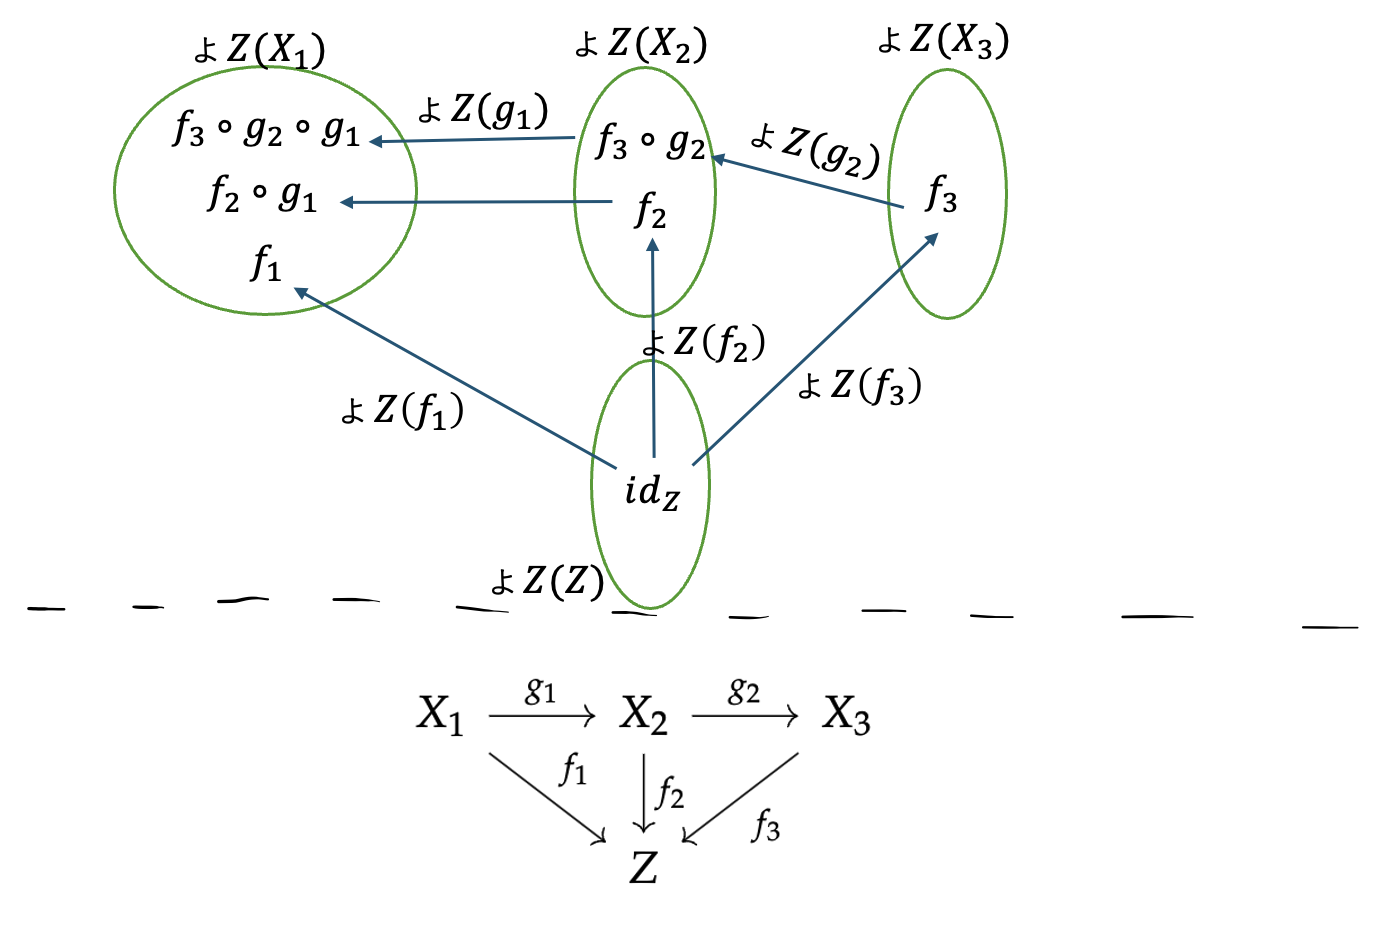
\includegraphics[width=300px]{fig/yo-1.png}
\end{center}

To build intuition, you should think of $\yo Z$ as describing ``the perspective
every other object in $\calC$ has on $Z$.'' Unpacking this more:
\begin{itemize}
  \item Let's look at the action of $\yo Z$ on $Z$ first.
  Unfolding the definition, we have:
  \begin{align*}
    (\yo Z)(Z) = \calC(Z, Z) = \{\id_Z\}
  \end{align*}
  So, somewhat vacuously, we might say: ``the perspective $Z$ has on itself 
  is the identity morphism''.
  And, for $X_1$, we have:
  \begin{align*}
    (\yo Z)(X_1) = \calC(X_1, Z) = \{f_1, f_2 \circ g_1, f_3 \circ g_2 \circ g_1 \}
  \end{align*}
  This is slightly more interesting: we would say, ``$X_1$ 
  has 3 perspectives on $Z$: (1) via the $f_1$ morphism, (2) by following 
  $f_2 \circ g_1$; (3) by following $f_3 \circ g_2 \circ g_1$''.
  \item Now let's look at the action on morphisms. These will correspond 
  to ``changes in perspective''. Let's examine the action of $\yo Z$ 
  on the morphism $f_1$:
  \begin{align*}
    (\yo Z)(f_1 : X_1 \to Z) &: \yo Z \to \yo X_1\\
    &= \id_Z \mapsto \id_z \circ f_1 = f_1
  \end{align*}
  One can understand this as: ``to move from ``$X_1$'s perspective on $Z$ 
  to $Z$'s perspective on $Z$, follow the $f_1$ morphism''. Somewhat 
  more interestingly, we can also shift perspectives between $X_1$
  and $X_2$ by precomposing with the $g_1$ morphism:
  \begin{align*}
    (\yo Z)(g_1 : X_1 \to X_2) &: (\yo Z)(X_2) \to (\yo Z)(X_1)\\
    &=
    \begin{cases}
      f_2 \mapsto f_2 \circ g_1 \\
      f_3 \circ g_2 \mapsto f_3 \circ g_2 \circ g_1
    \end{cases}
  \end{align*}
\end{itemize}

\subsection{Representables in the divisibility category}
Let's consider what representables look like in a familiar
category to get a better sense of their properties. Consider 
the following subset of the natural numbers ordered by 
divisibility:

\begin{center}
  % https://tikzcd.yichuanshen.de/#N4Igdg9gJgpgziAXAbVABwnAlgFyxMJZAJgBoAGAXVJADcBDAGwFcYkQBGYkAX1PUy58hFB1IdqdJq3YA2XvxAZseAkXKlikhizaIQ3PgJXCiZLTR0z9AZgXGhalDc3bpekAFZ7SwapEkpDZuuuwcvJIwUADm8ESgAGYAThAAtkieNDgQSGRSofoAxj7JaRlZOYgu+dYgAEYlKemImSDZSAAsNIz0dTCMAAp+pvqMMAk4IJbu7PSNZYh57YhiNR5Q883Vy6tWHmxGIKXNq8saa+wJETxAA
\begin{tikzcd}
  &                   & 12                                                &   \\
  & 6 \arrow[ru, "f"] &                                                   &   \\
2 \arrow[ru, "d"] &                   & 3 \arrow[lu, "e"]                                 & 5 \\
  &                   & 1 \arrow[llu, "c"] \arrow[u, "b"] \arrow[ru, "a"] &  
\end{tikzcd}
\end{center}

Let's consider the representables of each element in this category.
First let's inspect $\yo 12$. We can compute its action on objects:
\begin{align*}
  (\yo 12)(12) = \{\id_{12}\} \quad&
  (\yo 12)(6) = \{f\} \quad&
  (\yo 12)(3) = \{f \circ e\} \\
  (\yo 12)(2) = \{f \circ d\} \quad&
  (\yo 12)(1) = \{f \circ d \circ c\} \quad &
  (\yo 12)(5) = \{\}
\end{align*}

Note that in this category there is at most 1 morphism between any 2 objects
(i.e., we have that the morphisms $f \circ d \circ c = f \circ e \circ b$, 
so we only include 1 of them in $(\yo 12)(1)$).  So, each representable $\yo X$ is either a singleton (meaning, $X \preceq
12$), or it is an empty set (meaning $X \not\preceq 12$). The action of $\yo 12$
on morphisms is not complicated, let's see what it is by unfolding definitions:
\begin{align*}
  (\yo 12)(c) &: (\yo 12)(2) \to (\yo 12) (1) \\
  &= (f \circ d) \mapsto (f \circ d) \circ c
\end{align*}

In this case we see that to shift perspective from $1$ to $2$, we should 
precompose by the $c$ morphism.
From this, we can observe that there is single morphism $\yo Y \to \yo X$ 
if and only if there is a morphism $X \to Y$ in $\calC$.

Now, let's closely examine the structure of a representable $\yo 12$ and try 
to gain a more global picture of what data it contains. We can summarize 
$\yo 12$ by the following balloon, where we've replaced each object 
by its balloon:

\begin{center}
  % https://tikzcd.yichuanshen.de/#N4Igdg9gJgpgziAXAbVABwnAlgFyxMJZAJgBoAGAXVJADcBDAGwFcYkQAdD4LuHegE5cAviGGl0mXPkIoAjKTnU6TVuy48OfQSLESQGbHgJFypYsoYs2iTt178hHUeMlGZRMhZpW1tjQ46znpu0iYoZADMlqo2dpraTi76hmGyyAAs5jHW6vbBwsowUADm8ESgAGYCEAC2SGYgOBBIcq4g1XWtNM1IxO2d9YgKTS2IkQM1Q2SjSBmTXeM9Y-P6g0gArMtzhcJAA
\begin{tikzcd}
  &                                 & \{\star\} \arrow[ld] &  &                  \\
  & \{\star\} \arrow[ld] \arrow[rd] &                      &  &                  \\
\{\star\} \arrow[rrd] &                                 & \{\star\} \arrow[d]  &  & \{\} \arrow[lld] \\
  &                                 & \{\star\}            &  &                 
\end{tikzcd}
\end{center}

We see that the collection of objects with a $\star$ in them are exactly those objects 
that are at or below 12 in the order. This collection of objects has a name in 
order theory: it is called the \textbf{principal ideal} of 12. Formally:

\begin{definition}[Principal ideal]
  Let $(X, \le)$ be a preorder. Then, the \textbf{principal ideal} 
  of an element $a \in X$, written $\downarrow a$, 
  is the smallest collection of all elements less than or equal to $a$ 
  in $X$, i.e. 
  $\downarrow a = \{x \in X \mid x \le a\}$.
\end{definition}

So, we can summarize:
the representable $\yo 12$ is the principal ideal $\downarrow 12$, i.e.,
it contains exactly as much information as is contained in the principal ideal of 12. In general,
for any category formed by a preorder, it is the case that the representable of an 
element is a principal ideal in the preorder.
This order-theoretic viewpoint sheds some light on the intuition that the representable of an 
element is ``all the ways of viewing the element in the category''. One can imagine 
``peering up'' at an element $X$ from all the other objects: $\yo X$ is then all the vantage points below $X$ from 
which it can be seen.

\section{Representables in STLC}
So far we've been studying representables in thin categories, where there is a 
very pleasant order-theoretic understanding what they mean in terms of principal ideals.
Let's see an example of representables in a category with more than 1 morphism 
between objects.
Recall the syntax of \textsc{stlc}:
\begin{gather}
  \begin{aligned}
   A,B &::= \plkw{Unit}
     \mid A \pltimes B
     \mid A \plto B
  \\
  M,N &::= \plunit{}
      \mid \plpair{M}{N}
      \mid \plfst{M}
      \mid \plsnd{M}
      \mid \pllam{x}{M}
      \mid \plapp{M}{N}
      \mid x
  \end{aligned}
  \tag{\textsc{stlc}}
\end{gather}

Recall the category of simply-typed lambda calculus terms quotiented by 
equations:
\begin{definition}[The category STLC]
  The category of simply-typed lambda calculus terms (\textsc{stlc}) 
  is the category where:
  \begin{itemize}
    \item Objects are types $A$;
    \item Morphisms $A \to B$ are equivalence classes of terms $[x : A \vdash e : B]$ 
    where equality is given by the equational theory of the $\beta$ and $\eta$ laws;
    \item Composition is given by substitution:
    \begin{align*}
      [b : B \vdash N : C] \circ [a : A \vdash M : B] = [a : A \vdash N[M/b] : C]
    \end{align*}
    \item The identity morphism is the class of terms $[a : A \vdash a : A]$.
  \end{itemize}
\end{definition}

Let's see the representables in this category. 
For example, what do the representables $\yo (\plUnit \times \plUnit)$ look like?
Considering a concrete example:
\begin{align*}
  \yo (\plUnit \times \plUnit)(\plUnit) 
  &= \{\text{the ways of viewing terms of type $\plUnit \times \plUnit$ from terms of type $\plUnit$}\} \\ 
  &= \{[a : \plUnit \vdash M : \plUnit \times \plUnit] \mid M \text{ an stlc term}\}\\ 
  &= [a : \plUnit \vdash \plpair{a}{a} : \plUnit \times \plUnit]
\end{align*}

In the case above, there is only 1 element of the set $\yo (\plUnit \times \plUnit)(\plUnit)$: 
this is a quirk of our choice of types.
Intuitively, the representables $(\yo B)(A)$ for two types $A$ and $B$ 
is the collection of all equivalence classes of terms $M$ of type $A \to B$.
Then, naturally, the action on morphisms $(\yo X)(f : A \to B) : \yo B \to \yo A$ 
ought to be the ways of shifting viewpoints from $B$ to $A$,
i.e.:

\begin{align*}
  (\yo X)([a : A \vdash M : B]) &: (\yo X)(B) \to (\yo X)(A) \\
  &= [b : B \vdash N : X] \mapsto [b : B \vdash N : X] \circ [a : A \vdash O : B]  \\
  &= [b : B \vdash N : X] \mapsto [a : A \vdash N[O/b] : X]
\end{align*}

Carefully check all the types in the above equations.

\section{Representability}

There can be many $\calC$-indexed sets for a category, but the representables
are very special due to their relationship with the indexing category.
As usual in category theory, we are concerned not with particular objects 
but rather with equivalence classes of objects up to isomorphism,
a notion we make formal here:

\begin{definition}[Isomorphism of $\calC$-indexed sets]
  Two \(\calC\)-indexed sets \(P,Q\)
  are \emph{isomorphic}
if there are \(\calC\)-indexed functions \(\alpha : P \Rightarrow Q\)
and \(\beta : Q \Rightarrow P\)
such that \(\alpha\circ\beta=\idt_Q\) and \(\beta\circ\alpha=\idt_P\).
\end{definition}

With this definition in hand we can make precise the set of $\calC$-indexed 
sets that are tied to the indexing category:

\begin{definition}[Representability]
  \sloppy
  A \(\calC\)-indexed set \(P\) is \emph{representable}
  if there is an isomorphism \(\alpha : P \cong \yo X : \beta\)
  for some object \(X\) of \(\calC\).
\end{definition}

\begin{proposition}
  The \(\FinSet\)-indexed set \(\yo X \times \yo Y\)
  is representable.
\end{proposition}
\begin{proof}
  for any finite set \(A\), there is an isomorphism of sets
  \[
  \alpha_A : \FinSet(A,X \times Y) \cong \FinSet(A,X) \times \FinSet(A,Y).
  \]
  Concretely, \(\alpha_A\) is the function that sends
  a \(f \in \FinSet(A,X\times Y)\) to \((\pi_1 \circ f ,\pi_2,\circ f): \FinSet(A,X) \times \FinSet(A,Y) \).
  Its inverse is defined by \(\beta_A(f,g) = \angled{f,g}\).
  Both \(\alpha\) and \(\beta\) can be checked satisfy the naturality condition.
  Thus \(X\times Y\) represents \(\yo X \times \yo Y\).
\end{proof}

Representability is the bridge between
the internal view and the external view of a category: it lets us reflect 
properties presheaf category on $\calC$ back into $\calC$ itself. Concretely,
in the next chapter, we will use the Yoneda lemma in full to show:

\begin{theorem}
  Let $P,A,B$ be objects in a category $\calC$.  Then, $P$ is a product of $A$
  and $B$ if and only if it represents the product in the presheaf category $\yo A \times \yo B$.
\end{theorem}

We will not prove this theorem here -- it is a direct consequence of the 
Yoneda lemma, which we are now ready to appreciate -- but
one can understand this theorem as: an object $P$ is a product of $A$ 
and $B$ internally if and only if if behaves like a product externally.

% \section{The category of elements}

%% \section{$\calC$-indexed sets}

%% Let's begin by studying the category $\mathbb{N}^\infty$, the category
%% constructed from the preorder formed by the natural numbers extended by
%% infinity:

%% \begin{center}
%% \begin{tikzpicture}[
%% ]
%% % Objects (circles)
%% \node[minimum size=0.6cm] (o1) at (0,-1) {0};
%% \node[minimum size=0.6cm] (o2) at (1.5,-1) {1};
%% \node[minimum size=0.6cm] (o3) at (3,-1) {2};
%% \node (dots) at (4.2,-1) {$\cdots$};

%% % Arrows between objects
%% \draw[->] (o1) -- node[above] {$f$} (o2);
%% \draw[->] (o2) -- node[above] {$g$} (o3);
%% \draw[->] (o3) -- (dots);

%% \draw[->] (o1) edge[loop above] node[above] {$\id_0$} (o1);
%% \draw[->] (o2) edge[loop above] node[above] {$\id_1$} (o2);
%% \draw[->] (o3) edge[loop above] node[above] {$\id_2$} (o3);
%% \end{tikzpicture}
%% \end{center}

%% Given a category $\calC$, a $\calC$-indexed set associates each object of
%% a category with a set.
%% Let's consider a concrete $\calC$-indexed set called $F$.
%% We can draw $F$ as a ``balloon picture'' like this:

%% \begin{center}
%%   \includegraphics[width=175px]{fig/balloon-1.png}
%% \end{center}

%% Above each object is drawn a (in this case, finite) set.
%% $F_1$ is the set $\{a, b, c\}$, and $F_2$ is is the set
%% $\{d, e\}$.
%% In addition to associating each object with a set,
%% a $\calC$-indexed set also associates each morphism $X \mor{f} Y$
%% with a function $F_Y \to F_X$, which we can draw on the balloon
%% picture like so:

%% \begin{center}
%% \includegraphics[width=175px]{fig/balloon-2.png}
%% \end{center}

%% Intuitively, we can see that $F$ is describing a relation between two
%% categories: our category of interest $\calC$, and an ``external''
%% category of sets and functions. This relation is called a \textbf{functor}.
%% Functors have actions on objects

% \begin{tikzpicture}[
%   node distance=1.5cm,
%   morphism/.style={-Stealth, thick}
% ]

% % Top row of labels
% \node (v) at (0,2) {$v$};
% \node (c) at (3,2) {$c$};

% % Middle row
% \node (y) at (-1.5,1) {$y$};
% \node (w) at (0,1) {$w$};
% \node (a) at (3,1) {$a$};

% % Bottom row (just above the objects)
% \node (x) at (-1.5,0) {$x$};
% \node (h) at (0,0) {$h$};
% \node (b) at (3,0) {$b$};

% % Objects (circles)
% \node[circle, draw, minimum size=0.6cm] (o1) at (0,-1) {0};
% \node[circle, draw, minimum size=0.6cm] (o2) at (1.5,-1) {1};
% \node[circle, draw, minimum size=0.6cm] (o3) at (3,-1) {2};
% \node (dots) at (4.2,-1) {$\cdots$};

% % Arrows between objects
% \draw[morphism] (o1) -- (o2);
% \draw[morphism] (o2) -- (o3);
% \draw[morphism] (o3) -- (dots);

% \end{tikzpicture}




% \begin{center}
%  \begin{tikzpicture}[]

% % Objects
% \node (A) at (0,0) {$A$};
% \node (B) at (3,0) {$B$};
% \node (C) at (1.5,2.5) {$C$};

% % Identity morphisms (loops)
% \draw[->] (A) edge[loop left] node[left] {$\text{id}_A$} (A);
% \draw[->] (B) edge[loop right] node[right] {$\text{id}_B$} (B);
% \draw[->] (C) edge[loop above] node[above] {$\text{id}_C$} (C);

% % Morphisms between objects
% \draw[->] (A) -- node[below] {$f$} (B);
% \draw[->] (A) -- node[left] {$g$} (C);
% \draw[->] (C) -- node[right] {$h$} (B);
% \node[draw, fit=(A)(B)(C), inner sep=1cm, rectangle] {};
% \end{tikzpicture}
% \end{center}


%% Throughout this section we will work with an arbitrary category \(\calC\).

%% \begin{definition}[$\calC$-indexed set]
%%   A $\calC$-indexed set is a functor $F : \calC^\text{op} \Rightarrow \Set$.
%% \end{definition}

%% \begin{example}
%%   Recall that \(\mathsf{STLC}\) is a category
%%   whose objects are types and whose morphisms \(A \to B\)
%%   are terms \(x : A \vdash M : B\) quotiented by \(\beta\eta\)-equivalence.
%%   For each type \(A\),
%%   the following defines a \(\mathsf{STLC}\)-indexed set \(\mathsf{Tm}(A)\):
%%   \begin{align}
%%   \mathsf{Tm}(B)(A) &= \text{the set of morphisms \(A\to B\)} \\
%%   \mathsf{Tm}(B)(N : A'\to A)
%%   &= (x\ofty A \vdash M : B) \mapsto (x'\ofty A' \vdash M[N/x] : B)
%%   \end{align}
%% \end{example}
%% This example is a special case of a canonical kind of \(\calC\)-indexed set.
%% \begin{definition}
%%   The \emph{representable \(\calC\)-indexed set at \(X\)}
%%   is written \(\yo X\) and defined by
%%   \begin{align}
%%     (\yo X)(A) &= \text{the set of morphisms \(A \to X\)} \\
%%     (\yo X)(A)(s : A' \to A) &= (f : A \to X) \mapsto (f \circ s : A' \to X)
%%   \end{align}
%% \end{definition}

%% \begin{definition}
%%   \sloppy
%%   Let \(P\) and \(Q\) be \(\calC\)-indexed sets.
%%   A \emph{\(\calC\)-indexed function}
%%   from \(P\) to \(Q\),
%%   written \(\alpha : P \Rightarrow Q\),
%%   is a family of functions \(\alpha_X : PX \to QX\)
%%   that ``respects substitution''
%%   in the sense that \(\alpha_{X'}(x\cdot_P p) = \alpha_X(x)\cdot_p p\).
%% \end{definition}

%% \begin{itemize}
%% \item \(\calC\)-indexed functions can be composed:
%%   the composition of \(\alpha : Q \Rightarrow R\)
%%   and \(\beta: P \Rightarrow Q\),
%%   written \(\alpha\circ\beta : P \Rightarrow R\),
%%   is defined by \((\alpha\circ\beta)_X = \alpha_X \circ \beta_X\).
%% \item For each \(\calC\)-indexed set \(P\),
%%   there is a \(\calC\)-indexed function \(\idt_P : P \Rightarrow P\)
%%   defined by \(\idt_{P,X} = \left(PX \xrightarrow{\idt_{PX}} PX\right)\).
%% \end{itemize}
%% By now you may have noticed that \(\calC\)-indexed sets and functions
%% look like they ought to form a category. More on this later.

%% \begin{definition}
%%   Two \(\calC\)-indexed sets \(P,Q\)
%%   are \emph{isomorphic}
%% if there are \(\calC\)-indexed functions \(\alpha : P \Rightarrow Q\)
%% and \(\beta : Q \Rightarrow P\)
%% such that \(\alpha\circ\beta=\idt_Q\) and \(\beta\circ\alpha=\idt_P\).
%% \end{definition}

%% \begin{definition}
%%   A \(\calC\)-indexed set \(P\) is \emph{representable}
%%   if there is an isomorphism \(\alpha : P \cong \yo X : \beta\)
%%   for some object \(X\) of \(\calC\).
%% \end{definition}


\chapter{Yoneda IV: universal constructions, elements, and properties}

Now we are ready to appreciate the Yoneda lemma:

\begin{theorem}[Baby Yoneda]
  Let $\calC$ be a category, $X$ be an object in $\calC$, and $P$ 
  be a $\calC$-indexed set. Then, there is a bijective correspondence:\footnote{This 
  is called the ``baby Yoneda lemma'' because the full Yoneda lemma further stipulates 
  that this isomorphism satisfies additional naturality conditions. The baby Yoneda 
  lemma is still quite strong, however, and is much easier to prove.}
  \begin{align*}
    \{\text{$\calC$-indexed functions }\yo X \Rightarrow P\} \cong P(X)
  \end{align*}
  \label{thm:baby-yo}
\end{theorem}

On first glance this theorem is profoundly mysterious because it stipulates 
that there is a very strong relationship between two very different-seeming 
things. Let's unpack this slowly to really understand what is going on 
by instantiating the Yoneda lemma to a specific category and 
$\calC$-indexed set.
Let's consider a finite category with 3 objects:

\begin{equation}
  % https://tikzcd.yichuanshen.de/#N4Igdg9gJgpgziAXAbVABwnAlgFyxMJZABgBpiBdUkANwEMAbAVxiRAA0QBfU9TXfIRQBGclVqMWbAJrdeIDNjwEiAJjHV6zVohAAtbuJhQA5vCKgAZgCcIAWyRkQOCEmE8rth4lHPXiVS4KLiA
\begin{tikzcd}
  X \arrow[r, "f"] & Y \arrow[r, "g"] & Z
  \end{tikzcd}
\end{equation}

Now, let's define a simple $\calC$-indexed set $P$:
\begin{align*}
  P(X) = \{a, b\} \quad 
  P(Y) = \{c, d\} \quad
  P(Z) = \{e, h\} \\
  P(f) = \begin{cases}
    c \mapsto a \\
    d \mapsto b
  \end{cases}
  \quad 
  P(g) = \begin{cases}
    e \mapsto c \\
    h \mapsto d
  \end{cases}
\end{align*}

Continuing to unpack the data, we can define $\yo Z$, which is 
also a $\calC$-indexed set:

\begin{align*}
  (\yo Z)(Z) = \{\id_Z\} \quad
  (\yo Z)(Y) = \{g\} \quad
  (\yo Z)(X) = \{g \circ f\}
  \\
  (\yo Z)(f) = g \mapsto f \circ g \quad
  (\yo Z)(g) = \id_Z \mapsto f
\end{align*}

Next, let's enumerate the natural transformations $\yo X \Rightarrow P$
If the Yoneda lemma is true, we don't have too much work to do: 
we know there should be \emph{only two of them}, since $P(X)$ 
has only two elements in it. Let's enumerate them on a balloon diagram:

\begin{fullwidth}
  \begin{center}
    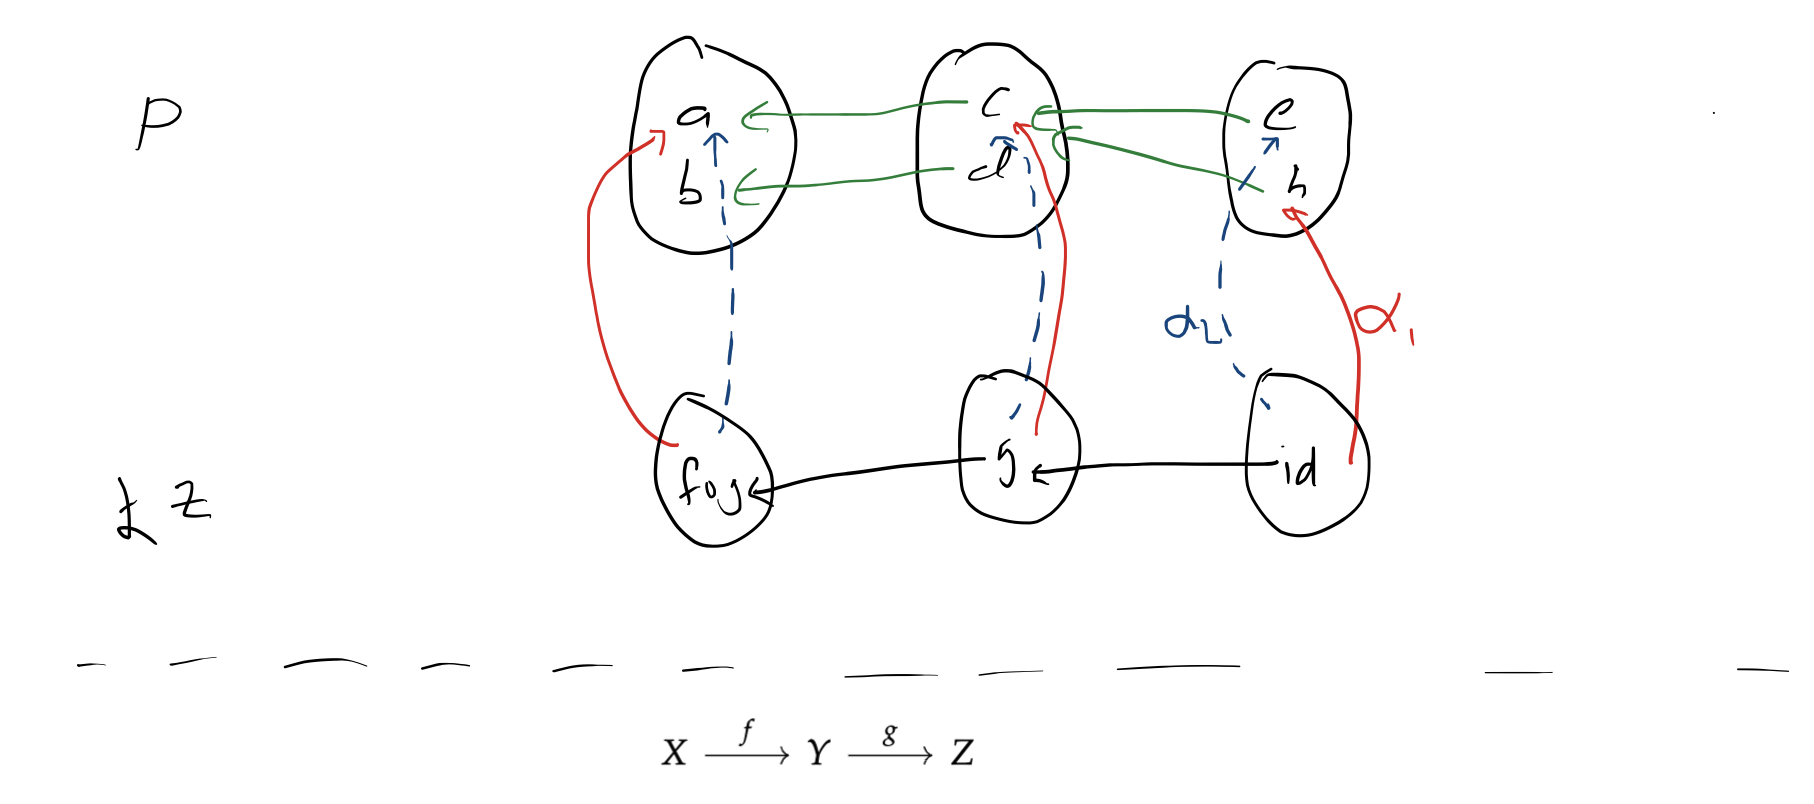
\includegraphics[width=400px]{fig/yo-2.png}
  \end{center}
\end{fullwidth}

Here we've drawn the two possible natural transformations $\alpha_1$ and
$\alpha_2$ in solid red and dashed blue respectively.  Now, let's understand why
the Yoneda lemma holds by tracing the possible paths through this balloon
diagram with your fingers.  Recall the two finger rule: a $\calC$-indexed
function $\yo Z \Rightarrow P$ satisfies the naturality condition if, starting
at any element in any balloon $\yo X$, your two fingers move in synchrony along
all possible paths.
So, let's start with $\yo Z = \{\id_Z\}$. Let's play the two finger game together
to design the two possible natural transformations:
\begin{itemize}
  \item Your left finger moves to $g$. Where can your right finger go? 
  It can go either to $e$ or $h$. So, choose $h$ and so we are designing $\alpha_1$. \emph{The rest of the 
  moves are forced}: your right finger must now move to $c$,
  then to $a$. Your left finger is also forced: it must move to $g$ 
  then to $f \circ g$. Now, all other decisions are forced, and we 
  can fill in $\alpha_1$ so that all moves are in harmony.
  \item Next, we can choose moving our right finger to $e$, and so 
  we are designing $\alpha_2$. \emph{Again, all moves are forced}: 
  the right finger follows the functions in $P$, and the left finger 
  follows the functions in $\yo Z$. Then, we are forced to choose 
  each $\alpha$ to exactly line up exactly with how these fingers move: 
  there is only one choice for $\alpha$ at each step.
\end{itemize}

Notice what is happening: because, in this example, 
there is a single element in $(\yo Z)(Z)$, then there must be 
\emph{exactly 1} natural transformation for each possible 
element in $P(Z)$. Naturality is a very strong restraint 
to place on $\alpha$!

So, it is now hopefully quite clear that, if $\id_Z$ is the only element of $\yo
Z$, the baby Yoneda lemma is true, since the entire action of a natural
transformation is determined by its action on the identity morphism of $Z$. But,
what if there is more than one morphism in $(\yo Z)(Z)$?

The crux is that the choice of \emph{$(\yo Z)(\id_Z)$} fully determines the
action of $\yo Z$ on all the other morphisms $Z \to Z$. Let's see this visually. 
Suppose we have as our indexing category the monoid corresponding to the 
natural numbers mod 3 under addition. This category has a single object $\star$ and 
3 morphisms: the identity morphism $0$, $1, 2$, where $1 \circ 1 = 2, 1 \circ 2 = \id, 2 \circ 2 = 1, 2 \circ 1 = \id$.
Let's visualize some of this data:

\begin{center}
  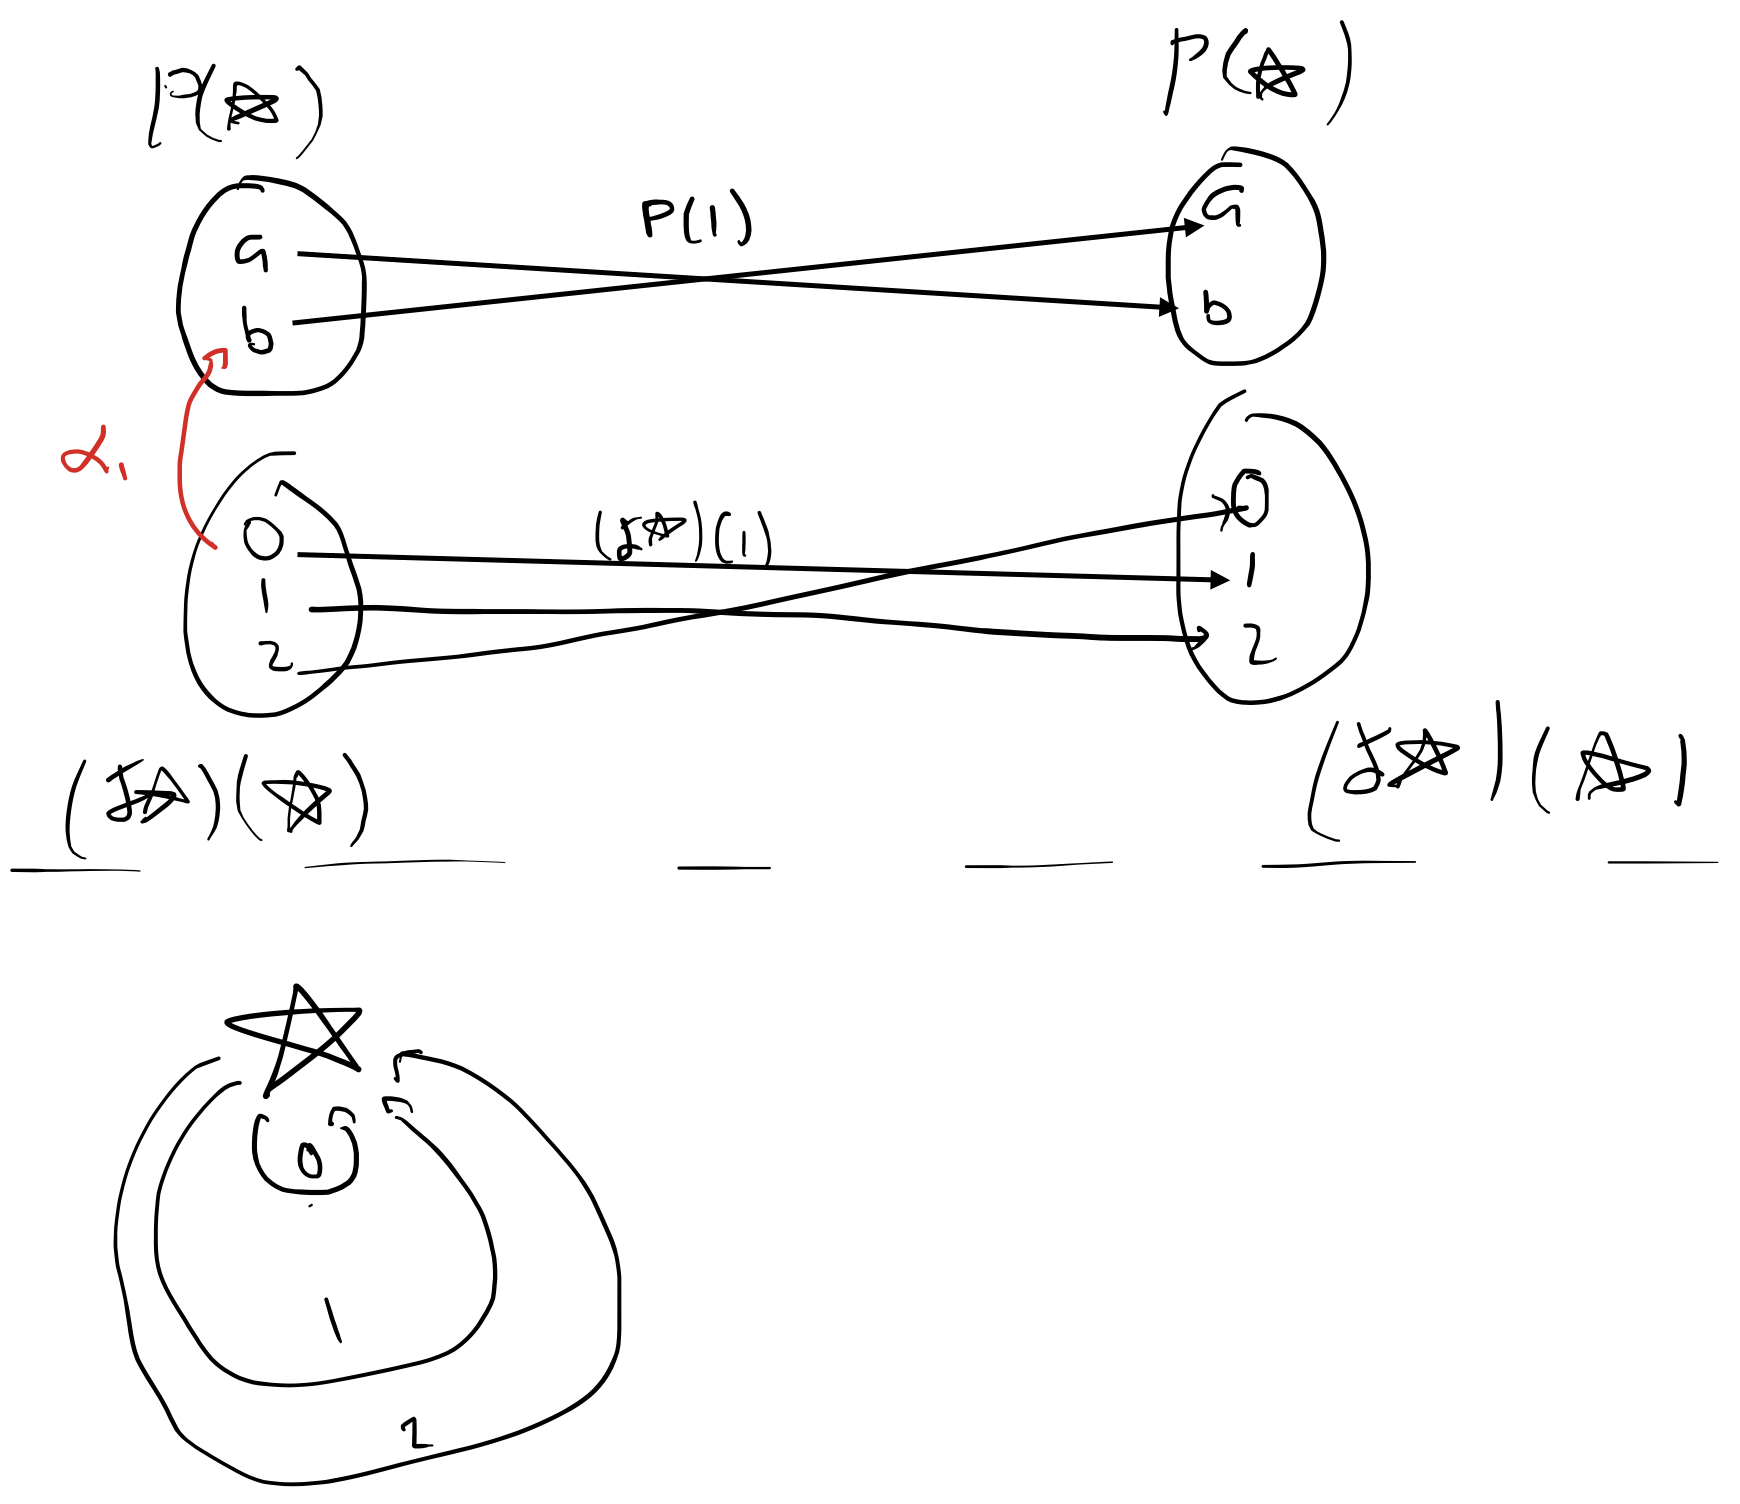
\includegraphics[width=250px]{fig/yo-3.png}
\end{center}

Here we've drawn an arbitrary $\calC$-indexed set $P$
with its action on the $1$ morphism, and we've chosen arbitrarily that
the $\calC$-indexed function
$\alpha_1$ maps $0$ to $b$. 
Note that we've drawn the balloon twice for the same object; this is for visualization 
purposes only.
Now, the key: \emph{does this choice of $\alpha$ 
fully determine how $\alpha$ behaves on all other elements of $(\yo \star)(\star)$}?
Indeed it does! Observe: by naturality, we have that $\alpha_1(1) = a$, which 
we can see by composing $P(1)\circ\alpha_1$. This gives us one more piece of data 
about $\alpha_1$. Now, what about $\alpha_1(2)$? We can get this piece of data 
by inspecting $P(2)$ and $(\yo \star)(2)$:

\begin{center}
  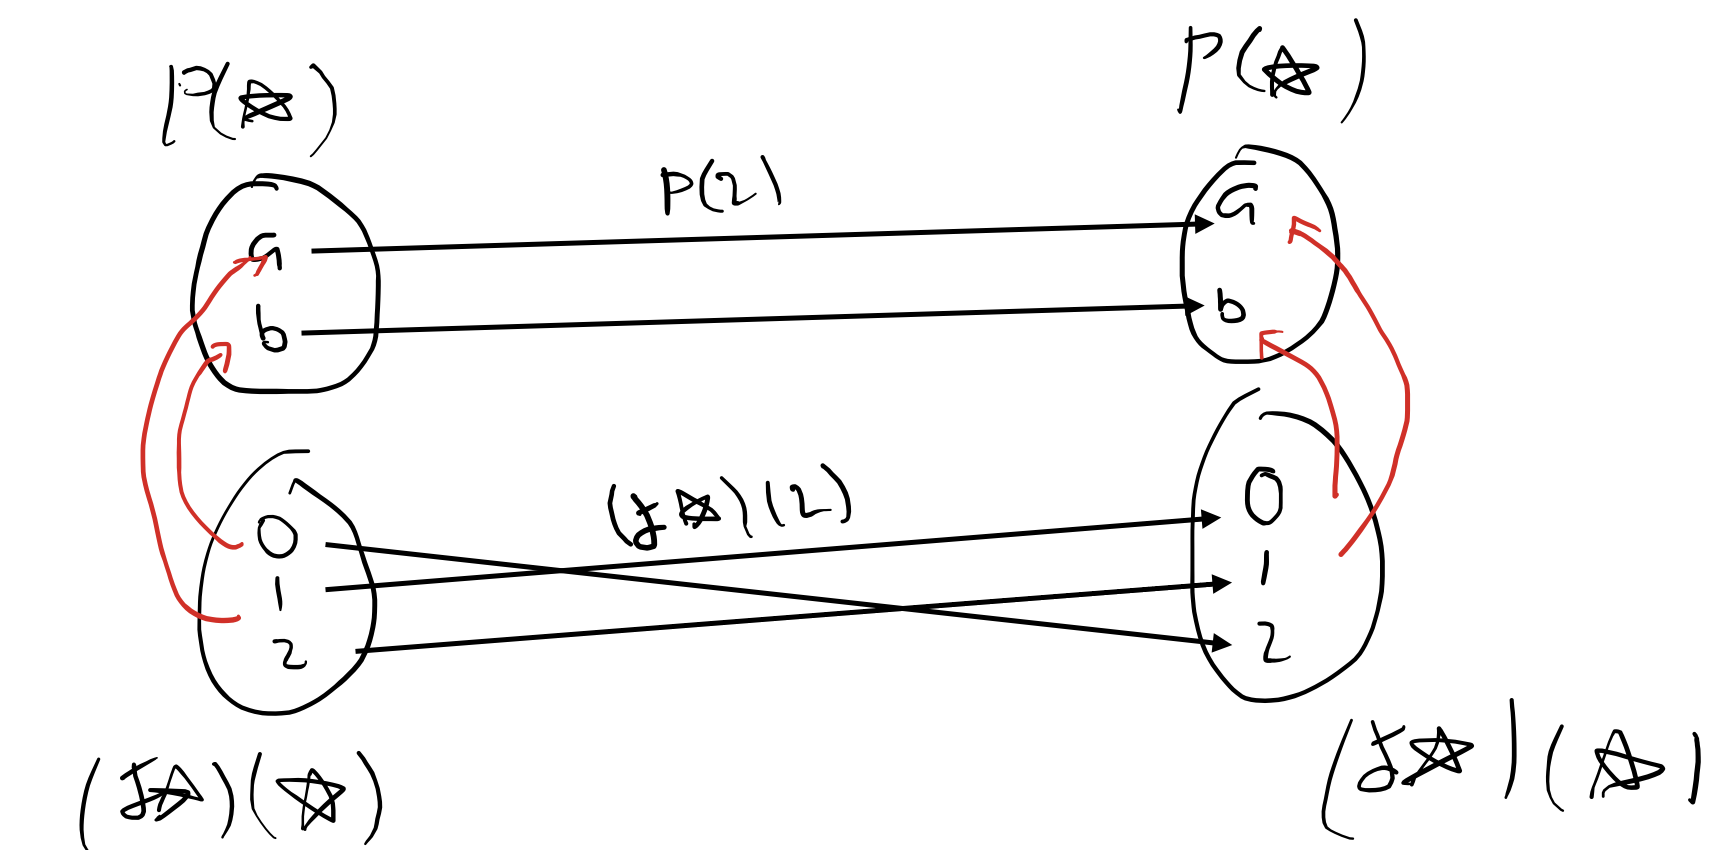
\includegraphics[width=250px]{fig/yo-4.png}
\end{center}

And now here we learn the final component of $\alpha$: we conclude that $\alpha(2) = b$.

\section{Proving the baby Yoneda lemma}
\marginnote{Thanks to Bex Golinov for the scribe notes for the next two subsections. \todo{} these can be tidied 
up a bit.}
Now we are ready to prove \cref{thm:baby-yo}. Let $\calC$ be a 
category, $P$ be a $\calC$-indexed set, and $X$ be an object 
in $\calC$. Then, we need to construct a bijection:

\begin{center}
  % https://tikzcd.yichuanshen.de/#N4Igdg9gJgpgziAXAbVABwnAlgFyxMJZABgBpiBdUkANwEMAbAVxiRAB13hOBfEH0uky58hFAEZyVWoxZsACgAoAGgEp+0mFADm8IqABmAJwgBbJGRA4ISSSABGMMFCQBmS-WatEIbf0Egxma21NYW1I7ObpYMdI4M8sJ4BGwMMAY4INSecj4GTGAAxho8QA
\begin{tikzcd}
  \{\calC\text{-indexed functions }\yo X \Rightarrow P\} \arrow[r, "g", bend left] & P(X) \arrow[l, "func", bend left]
  \end{tikzcd}
\end{center}

\newcommand{\fun}{func}
\newcommand{\cat}{\mathcal{C}}
What does this bijective correspondence statement actually mean? We have some
$\fun$ that, given a $p\in PX,$ can construct a natural transformation $\alpha:
\yo X \Rightarrow P$, and some $g$ that can extract $p$ from a given natural
transformation.
\begin{enumerate}
    \item Constructing natural transformation from $p\in PX$
    \begin{itemize}
        \item Given a $p\in PX$, we defined
        $\fun(p)$ via a family of functions $\fun(p)_A,$ where $\fun(p)$ is a
        natural transformation. We can think of the $\fun(p)_A$ as the
        components of $\fun(p),$ where for each object $A$ in $\cat,$ the
        component $\fun(p)_A$ maps from $(\yo X )(A)$ to $P(A)$. 
    \begin{align*}
        \fun(p)_A : &(\yo X)(A) \to PA\\
        &f \mapsto (Pf)(p)
    \end{align*}
    where $f:A \to \yo X$. The element $p$ by definition has type $PX,$ and $P$ is contravariant so $Pf$ maps $PX$ to $PA,$ giving us the desired codomain.
    \item Naturality of $\fun(p)$. Let $g:B\to A$. I don't really want to justify this but here is the square
    \[
\begin{tikzcd}[column sep=large, row sep=large]
(\yo X)(A) \arrow[r, "\fun(p)_A"] \arrow[d, "(\yo X)(g)"'] & P(A) \arrow[d, "P(g)"] \\
(\yo X)(B) \arrow[r, "\fun(p)_B"'] & P(B)
\end{tikzcd}
\]
    \end{itemize}
    \item Getting $p$ from natural transformation
    \begin{itemize}
    \item How did we extract $p\in PX$ from some given natural transformation $\alpha$? We know $\alpha_X$ maps $(\yo X)(X) \to PX$, so applying $\alpha_X$ to $id_X$ gives us an element of $PX,$ we can set $p:=\alpha_X(id_X)$. 
    \item Now we need to show $\alpha_A = \fun(p)_A$. Since $\alpha_A$ acts on the elements of $(\yo X)(A)$, it suffices to show $\alpha_A(f) = \fun(p)_A = (Pf)(p)$ for every $f\in\cat(A,X)$.
    \item We have $(Pf)(p) = (Pf)(\alpha_X(id_X))$. We will use the naturality of $\alpha$. Specifically, $Pf \circ \alpha_X = \alpha_A \circ (\yo X)(f)$.
      \[
\begin{tikzcd}[column sep=large, row sep=large]
(\yo X)(X) \arrow[r, "\alpha_X"] \arrow[d, "(\yo X)(f)"'] & P(A) \arrow[d, "P(f)"] \\
(\yo X)(A) \arrow[r, "\alpha_A"'] & P(B)
\end{tikzcd}
\]
    \begin{align*}
        (Pf)(\alpha_X (id_X)) = (Pf \circ \alpha_A)(id_X) &= (\alpha_A \circ (\yo X)(f))(id_X)\\
        &= \alpha_A((\yo X)(f)(id_X)) = \alpha_A(id_x \circ f).\\
        &= \alpha_A(f)
    \end{align*}
    So $(Pf)(p) = \alpha_A(f)$, and we are done!
\end{itemize}
\end{enumerate}

\begin{remark}
    Defining some natural transformation $\alpha := f(p)$ by defining how $f(p)$ acts on each object $A$ is like a "pointwise" definition of $\alpha$. 
\end{remark}

\section{The category of elements}
\begin{definition}[Category of elements]
    The \textit{category of elements} of a $\cat$-indexed set has 
    \begin{enumerate}
        \item objects : pairs $(X,p\in PX)$
        \item morphisms : from $(X,p\in PX)$ to $(Y,q\in PY)$ are morphisms
        $f:X\to Y$ of $\cat$ such that $(Pf)(q) = p$. Alternatively, $q \cdot_P
        f = p$. A morphism of this category of elements is a morphism from the
        original category with the \textit{additional} structure of preserving
        the points of $PX$.
    \end{enumerate}
    Definitions of composition and identity follow immediately from the
    definitions in $\cat,$ with the additional restriction of point
    preservation. It is relatively simple to show the desired categorical
    properties hold.
\end{definition}
\begin{proposition}
    Suppose $\cat$-indexed set $P$ is representable by $X$. There exists a $u\in
    PX$ called the \textit{P-universal element} which satisfies the following
    universal property : for any object $\Gamma$ of $\cat$ and any $g\in
    P\Gamma,$ there exists a unique $\hat{g}:\Gamma\to X$ such that $g = u
    \cdot_P \hat{g}$. Alternatively, $g = (P\hat{g})(u)$.
    \label{prop:univ-elem}
\end{proposition}
\begin{proposition}
    A $\cat$-indexed set $P$ is representable if $P\cong\yo X$ for some object
    $X$ of $\cat$. Suppose $P$ is representable. Then there exists a
    \textit{universal element} $u\in PX$ and $u$ is a terminal object in the
    \textit{category of elements} of $P$.
    \label{prop:univ-terminal}
\end{proposition}

We have from \cref{prop:univ-terminal} the definition of the universal property that we
want these mysterious universal elements to satisfy. We can think about this
definition as stating that we can ``factor'' any $g\in P\Gamma$ (for any $\Gamma$)
into $u$ and a unique $\hat{g}$.


What does it mean for $u \in P(X)$ to be terminal in the category of elements of
$P$? That any object has a unique morphism mapping to $(X,u)$. Explicitly, for
any $(A, p\in PA),$ there is a unique map $f:A \to X$ such that $(Pf)(u)=p$ (or
$p = u \cdot_P f)$. This looks pretty similar to the universal property given in
\cref{prop:univ-terminal} -- we can ``factor'' any $p\in PA$ into $f$ and $u$.


How do we get \cref{prop:univ-terminal} from the Yoneda Lemma? These are the key ideas:
\begin{itemize}
    \item $X$ representing $P$ means we have an isomorphism between $\yo X$ and $P$. This isomorphism is a $\cat-$indexed function, which we have learned is usually called a natural transformation. So technically we have a bijective natural transformation (a natural isomorphism?)
    \item The Yoneda Lemma says that for every natural transformation $\yo X \Rightarrow P,$ we should have a corresponding $u\in PX$ from which we can construct said transformation. This means the natural isomorphism between $\yo X$ and $P$ has a \textit{corresponding }$u\in PX$ (suggestively labeled). 
    %unsure if will include this next bullet, may give away the problem 
    %\item Let $\alpha$ denote the natural isomorphism $\yo X \Rightarrow P$.
    %Because $\alpha$ is bijective, and $\alpha$ can be defined component-wise,
    %each $\alpha_A$ for each object $A$ must also be bijective. So consider
    %this bijection $\alpha_A: (\yo X)(A)\Rightarrow PA$. From surjectivity, for
    %any $p\in PA,$ there exists some $\hat{p}$ in $(\yo X)(A)$ such that
    %$\alpha_A(\hat{p}) = p$. From injectivity, this $\hat{p}$ is unique. 
   % \item How do we connect this $\hat{p}$ to the corresponding $u\in PX$ we
   % identified? (Look at how we constructed the natural transformations
   % $\alpha_A$ in our proof of baby yoneda).
    % probably do not include
    %\item From Yoneda Lemma we know we have a function $\fun(p)$ defined as a
    %family of functions $\fun(p)_A$, where $\fun(p)_A$ maps $p$ to the
    %component $\alpha_A$. Specifically, $\alpha_A$ is defined to take elements
    %of $(\yo X)(A),$ e.g. some $f:A \to X,$ and map them to $(Pf)(p) = p
    %\cdot_P f$, elements of $PA$. Then we know $\alpha_A(\hat{p}) = u \cdot_P
    %\hat{p}$ and $\alpha_A(\hat{p})=p,$ meaning $p = u \cdot_P \hat{p}$ !
\end{itemize}



\section{Calculating a universal property}
\todo{Show how to calculate the universal property of 
a product}

% \section{Cayley's theorem}

% \begin{definition}
%   \sloppy
%   Given two \(\calC\)-indexed sets \(P\) and \(Q\),
%   their \emph{product} \(P\times Q\)
%   is the \(\calC\)-indexed set defined by
%   \((P\times Q)(X) = P(X)\times Q(X)\),
%   with substitution defined by
%   \((x,y)\cdot_{P\times Q} p = (x\cdot_P p, y\cdot_Q p)\).
% \end{definition}

% \begin{proposition}
%   Let \(X\) and \(Y\) be two objects of a category \(\calC\).
%   An object \(P\) is a product of \(X\) and \(Y\)
%   if and only if \(\yo P\) is isomorphic to \(\yo X \times \yo Y\).
% \end{proposition}

% \begin{definition}
%   Given two objects \(X\) and \(Y\) of a category \(\calC\),
%   there is a \(\calC\)-indexed set of \emph{closures},
%   written \(\mathsf{Clos}(X,Y)\),
%   defined by \(\mathsf{Clos}(X,Y)(\Gamma) = \calC(\Gamma\times X, Y)\),
%   with substitution defined by
%   \[
%     \mathsf{Clos}(X,Y)(s : \Gamma'\to \Gamma)(f : \Gamma\times X \to Y)
%     = \angled{\gamma',x} \mapsto f \circ \angled{s\circ \gamma', x}
%   \]
%   on generalized elements.
% \end{definition}

% \begin{proposition}
%   Let \(X\) and \(Y\) be two objects of a category \(\calC\).
%   An object \(E\) is the exponential \(Y^X\)
%   if and only if \(\yo E\) is isomorphic to \(\mathsf{Clos}(X,Y)\).
% \end{proposition}

% \begin{proposition}
%   Suppose the \(\calC\)-indexed set \(P\) is represented
%   by the object \(X\).
%   Then there exists an element \(u \in PX\),
%   called the \emph{\(P\)-universal element},
%   which satisfies the following \emph{universal property}:
%   for any object \(\Gamma\) and any element \(g \in P\Gamma\),
%   there exists a unique morphism \(\hat g : \Gamma \to X\)
%   such that \(g = u \cdot_P \hat g\).
% \end{proposition}

% \begin{itemize}
% \item In the case of the product, with \(\yo P \cong \yo X \times \yo Y\),
%   the universal element is an element \(u \in \calC(P,X) \times \calC(P,Y)\),
%   which is a pair of morphisms \(P\to X, P\to Y\).
%   The universal property of this pair is that any other pair \(\Gamma \to X,\Gamma\to Y\)
%   factors uniquely through it---precisely the universal property of products
% \item In the case of exponents, with \(\yo E \cong \calC(A\times(-),B)\),
%   the universal element is an element \(u \in \calC(A \times E,B)\),
%   which is a morphism \(A \times E \to B\).
%   The universal property of this morphism is that any other morphism
%   \(A \times \Gamma \to B\)
%   factors uniquely through it---precisely the universal property of exponents.
% \end{itemize}

\chapter{Functors and natural transformations}
We are ready to broaden our categorical perspective and language to begin 
comparing two categories with one another. We will see how some of the notions 
we've been encountering so far in our journey through the Yoneda 
lemma -- in particular, the functoriality and naturality properties of 
$\calC$-indexed sets and functions -- are special cases of more general 
phenomena in category theory called functors and natural transformations.


\section{Functors}
A functor is a structure-preserving map between categories:

\begin{definition}[Functor]
  \sloppy
  Given two categories \(\calC\) and \(\calD\),
  a \emph{functor \(F\) from \(\calC\) to \(\calD\)},
  written
  \(F : \calC \to \calD\),
  consists of \begin{itemize}
    \item An ``action on objects'', which is a function sending each object \(X\) of \(\calC\) to an object \(F(X)\) of \(\calD\)
    \item An ``action on morphisms'', which is a function sending each morphism \(X \mor{f} Y\) of \(\calC\) to a morphism \(F(X) \mor{F(f)} F(Y)\)
      of \(\calD\)
  \end{itemize}
  such that the following \emph{functoriality conditions} are satisfied:
  \begin{itemize}
  \item Identity preservation: for all objects \(X\) of \(\calC\) it holds that \(F(\idt_X) = \idt_{F(X)}\)
  \item Composition preservation: for all composable pairs of morphisms \(X \mor{f} Y \mor{g} Z\) of \(\calC\)
    it holds that \(F(g \circ f) = F(g) \circ F(f)\).
  \end{itemize}
\end{definition}

Intuitively, if there is a functor $F : \calC \to \calD$, then 
there is an ``abstract copy of $\calC$ inside $\calD$''. 

% Think back to \(\calC\)-indexed sets. We drew these as Balloon diagrams, with sets lying above objects of \(\calC\).
% It may help to think of the definition of functor as an ``abstract Balloon diagram'', where balloons are replaced by objects of \(\calD\):
% \[% https://tikzcd.yichuanshen.de/#N4Igdg9gJgpgziAXAbVABwnAlgFyxMJZABgBoBGAXVJADcBDAGwFcYkQANEAX1PU1z5CKchWp0mrdgE0efEBmx4CRMsXEMWbRCABiXXvyVCio9TU1Sdu2d3EwoAc3hFQAMwBOEALZIyIHAgkUQktdjcQGkZ6ACMYRgAFAWVhEA8sRwALHDl3L19EACYaQKQAZgtJbT0Iu24gA
% \begin{tikzcd}
% FX \arrow[r, "Ff"] & FY \\
% X \arrow[r, "f"']  & Y
% \end{tikzcd}\]



\subsection{Examples of functors}
The simplest example of a functor is one between two finite 
categories. Consider the following example of a functor 
between two finite categories $\calC$ and $\calD$:
\marginnote{A good exercise: how many functors are there 
from $\calC$ to $\calD$?}

\begin{center}
  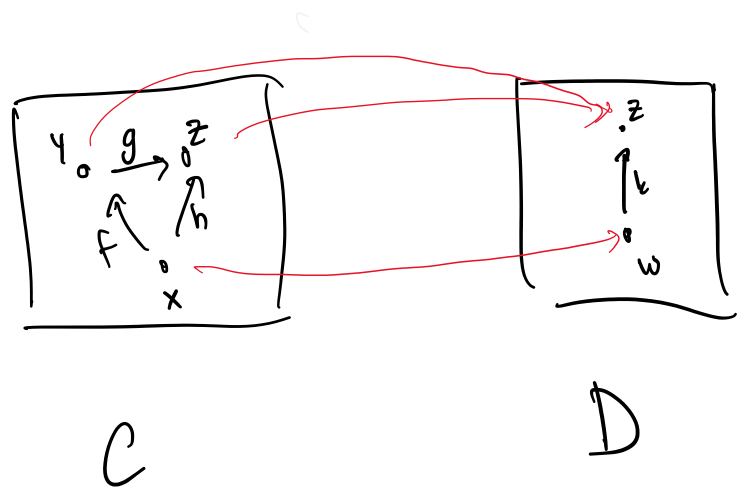
\includegraphics[width=0.5\linewidth]{fig/func-2.png}
\end{center}

The functor $F : \calC \to \calD$ is drawn in red; 
we've only shown its actions on objects here. Written out, 
we have:
\begin{align*}
  F(Y) = Z, \quad F(X) = W, \quad F(Z) = Z
\end{align*}
This action on objects defines the action on morphisms. 
This isn't always the case; there may be more than one morphism 
between two objects in $\calC$ and $\calD$, in which case, there may 
be a choice on which morphisms to map to. But here, it is simple,
and we can conclude:
\begin{align*}
  F(\id_Y) = \id_Z \quad F(\id_X) = \id_Z \quad F(\id_Z) = \id_Z \\
  F(g) = \id_Z \quad F(f) = k \quad F(h) = k
  \quad F(g \circ f) = k
\end{align*}

We need to check that the functoriality properties are 
satisfied. Clearly, identity preservation is satisfied. The only interesting 
case to check is the compositional property that $k = F(g \circ f) = F(g) \circ F(f) = \id_Z \circ k = k$.

As usual, it's useful to gain an intuition for what functors look like 
between categories that represent preorders. They will correspond to 
monotone functions:

\begin{definition}[Monotone function]
  Let $(X, \le_X)$ and $(Y, \le_Y)$ be preorders. Then, a 
  function $f : X \to Y$ is called \emph{monotone} if, 
  for any $x_1, x_2 \in X$ such that $x_1 \le_X x_2$, 
  it is the case that $f(x_1) \le_Y f(x_2)$.
\end{definition}

Now, let's see how functors between preorders correspond to monotone 
functions. 
Let $\calC$ and $\calD$ be categories corresponding to preorders
and let $F : \calC \Rightarrow \calD$ be a functor between 
these two categories.
Then, functoriality of $F$ requires that,
for any morphism $X \xrightarrow{f} Y$ in $\calC$, 
there is a morphism $F(X) \xrightarrow{f} F(Y)$.
This is exactly the monotonicity requirement:
the morphism $f$, considered order-theoretically, 
denotes that $X \le Y$; similarly, the morphism $F(f)$ 
denotes that $F(X) \le F(Y)$.



% Examples:
% \begin{itemize}
% \item Functors between two preorders are montone functions
% \item Denotational semantics of STLC is a functor \(\mathsf{STLC} \to \FinSet\)
% \item You may wonder: is a \(\calC\)-indexed set a functor? Hold that thought
% \end{itemize}


\section{Natural transformations}
Natural transformations are structure-preserving maps between functors:

\begin{definition}[Natural transformation]
  \sloppy
  Given two categories \(\calC\) and \(\calD\),
  and two functors \(F,G : \calC \to \calD\),
  a \emph{natural transformation \(\alpha\) from \(F\) to \(G\)},
  written
  \(\alpha : F \Rightarrow G\),
  consists of a function sending each object \(X\) of \(\calC\) to a \emph{morphism} \(F(X) \mor{\alpha_X} G(X)\) of \(\calD\)
  such that the following \emph{naturality condition} is satisfied:
  for each morphism \(X \mor{f} Y\) of \(\calC\), the following square commutes:
  \[
  % https://tikzcd.yichuanshen.de/#N4Igdg9gJgpgziAXAbVABwnAlgFyxMJZABgBpiBdUkANwEMAbAVxiRADEANEAX1PUy58hFGQCMVWoxZt2ATV78QGbHgJEx5SfWatEIAOLc+A1cI2kJ1HTP0GFPSTCgBzeEVAAzAE4QAtkhkIDgQSJpSurKeINQMdABGMAwACoJqIiDeWC4AFjiKXr4BiOEhSADM1tJ6IAA6tYxoOXQA+gqxCUmpZur6Wbn5JiA+-kgATNRliJURtobRQyPFQVMTszX1jc0txhQ8QA
\begin{tikzcd}
FX \arrow[d, "Ff"'] \arrow[r, "\alpha_X"] & GX \arrow[d, "Gf"] \\
FY \arrow[r, "\alpha_Y"']                 & GY
\end{tikzcd}
  \]
  In other words, \(\alpha_Y \circ Ff = Gf \circ \alpha_X\) for all \(X \mor{f} Y\).
\end{definition}

Let's consider two functors $F$ and $G$ between finite categories and a 
natural transformation $\alpha : F \Rightarrow G$:
\begin{center}
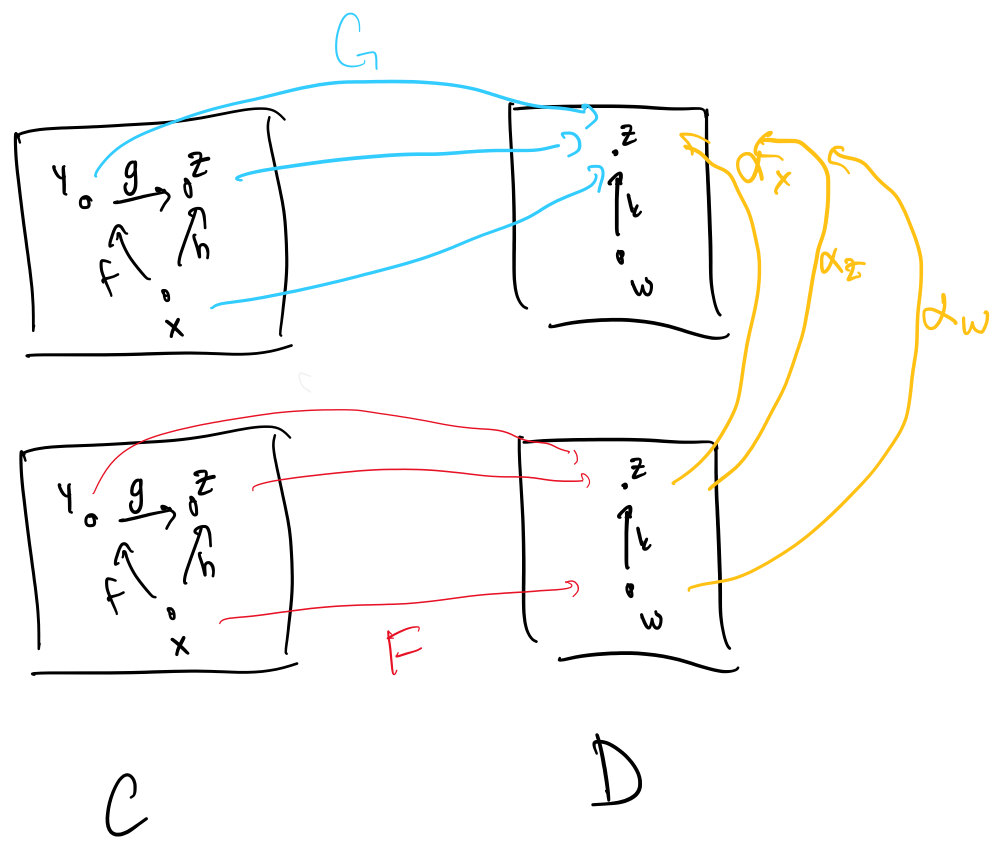
\includegraphics[width=0.8\linewidth]{fig/nat-trans1.png}
\end{center}

Breaking the data in this figure down, we have that $\alpha_X = \id_Z$, 
$\alpha_Z = \id_Z$, and $\alpha_W = k$. Now we can 
check the naturality square for every morphism:
\begin{itemize}
  \item Checking for $f$: we need to show that $\alpha_Y \circ F(f) = G(f) \circ \alpha_X$.
  Substituting, this is $\id_Z \circ k = \id_Z \circ k$.
\end{itemize}


\subsection{More examples of natural transformations}

Think back to \(\calC\)-indexed functions. We drew these as squares involving two Balloon diagrams stacked together.
It may help to think of the naturality condition as an abstraction of such a picture, where Balloons are replaced by
objects of \(\calD\):
\[% https://tikzcd.yichuanshen.de/#N4Igdg9gJgpgziAXAbVABwnAlgFyxMJZABgBoBmAXVJADcBDAGwFcYkQANEAX1PU1z5CKAIwVqdJq3YBNHnxAZseAkTIiJDFm0QgAYl179lQtaWKapOkAHFDCpYNWjSGmlum69co4oErhZDELdyt2Gx8JGCgAc3giUAAzACcIAFskMhAcCCQxSW12RPkk1IzEACYaHKQAFlDCr2KaRnoAIxhGAAV-U11krBiACxwSkBT0pHJq3MQAVgbPW2LfCfKq7NnpgqWAHV2mNCH6AH17UsnEes2kBZ3rfcPjk4BPEBb2zp6TZxAB4dG3Eo3CAA
\begin{tikzcd}
GX \arrow[r, "Gf"]                        & GY                        \\
FX \arrow[r, "Ff"'] \arrow[u, "\alpha_X"] & FY \arrow[u, "\alpha_y"'] \\
                                          &                           \\
X \arrow[r, "f"]                          & Y
\end{tikzcd}\]

\begin{definition}[Identity natural transformation]
  Let \(F : \calC \to \calD\) be a functor between two categories \(\calC,\calD\).
  The identity natural transformation \(\idt_F : F \Rightarrow F\)
  is defined by \(\idt_{F,X} = \idt_{F(X)}\).
  Naturality is verified by the following ``abstract balloon diagram'':
  \[% https://tikzcd.yichuanshen.de/#N4Igdg9gJgpgziAXAbVABwnAlgFyxMJZABgBoBmAXVJADcBDAGwFcYkQANEAX1PU1z5CKAIwVqdJq3YBNHnxAZseAkTIiJDFm0QgAYl179lQomI00t03XrlHFAlcJKlimqTv2GFSwatGu7trstjwSMFAA5vBEoABmAE4QALZIZCA4EEhiksG6cfLxSamIACw0mUgArJYeIQX2iSlIAEwVWYjktXn6DQpNJW0ZHeW51iAAOhNYUDgA+sAG3IUgA0hdw9Xd41Mz84syy9yU3EA
\begin{tikzcd}
FX \arrow[r, "Ff"]                        & FY                        \\
FX \arrow[r, "Ff"] \arrow[u, "\idt_{FX}"] & FY \arrow[u, "\idt_{FY}"] \\
                                          &                           \\
X \arrow[r, "f"]                          & Y
\end{tikzcd}\]
\end{definition}

\begin{definition}[Composition of natural transformations]
  Given \(\alpha : F \Rightarrow G\) and \(\beta : G \Rightarrow H\),
  the composition \(\beta\circ \alpha : F \Rightarrow H\) is defined by
  \((\beta\circ\alpha)_{X} = \beta_X \circ \alpha_X\).
  Naturality is verified by the following ``abstract balloon diagram'':
  \[% https://tikzcd.yichuanshen.de/#N4Igdg9gJgpgziAXAbVABwnAlgFyxMJZABgBoAWAXVJADcBDAGwFcYkQANEAX1PU1z5CKAIwVqdJq3YBNHnxAZseAkTIAmCQxZtEIAGJde-ZUKJjNNbdL365xxQJXCSpEVqm6QAcSMKlgqqibh467N72-k5mKGTEoTYgABJ+JoEuYvFWnuxJ9hIwUADm8ESgAGYAThAAtkhkIDgQSGKSYXrl8hXVdYjkNE1IAKzZ7T6dDlW1SOoDzYgAzKOJ+hMKU72zjfP9bYkAOvtMaAAW9AD6qSAbSEvbw8teh8dn53I0jPQARjCMAArRIIgSpYIonHBda49JC7QaIABsj3Yhx+OAuVxuiBG90QAHYkXoUTA0W8QB9vr8AaYgSCwRDJtCEXMkPi9l4khNKNwgA
\begin{tikzcd}
HX \arrow[r, "Hf"]                       & HY                        \\
GX \arrow[r, "Gf"] \arrow[u, "\beta_X"]  & GY \arrow[u, "\beta_Y"']  \\
FX \arrow[r, "Ff"] \arrow[u, "\alpha_X"] & FY \arrow[u, "\alpha_Y"'] \\
                                         &                           \\
X \arrow[r, "f"]                         & Y
\end{tikzcd}\]
\end{definition}

Examples
\begin{itemize}
\item Suppose you have two functors \(F,G : X \to Y\) between preorders \(X,Y\), aka two monotone functions.
  There is at most one natural transformation \(\alpha : F \Rightarrow G\), which exists if and only if \(F(x) \le G(x)\) for all \(x\in X\).

\item Mind-bending example: there is an identity functor \(\mathsf{id} : \FinSet \to \FinSet\).
  What does a natural transformation \(\alpha : \mathsf{id} \Rightarrow \mathsf{id}\) look like?
  Think polymorphism: intuitively, \(\alpha\) must have type ``\(\forall X. \FinSet(\mathsf{id}(X),\mathsf{id}(X))\)'',
  aka ``\(\forall X. X \to X\)''.
  This suggests that \(\alpha\) is the identity, i.e., \(\alpha_X = \idt_X\) for all objects \(X\) of \(\FinSet\).
  Indeed, we can verify this follows from \(\alpha\) being natural, as follows.
  \begin{itemize}
  \item Let \(X\) be an arbitrary object of \(\FinSet\). We will show \(\alpha_X\) is the identity function on \(X\).
  \item By function extensionality it's enough to show that for all \(x \in X\) it holds that \(\alpha_X(x) = x\).
  \item Fix \(x \in X\) arbitrary. We saw in a homework that \(x\) corresponds to a \(\FinSet\) morphism \(\hat x : 1 \to X\),
    where \(1\) is the terminal object of \(\FinSet\) (aka the one-point set).
    Now, by naturality of \(\alpha\), the following square commutes:
    \[% https://tikzcd.yichuanshen.de/#N4Igdg9gJgpgziAXAbVABwnAlgFyxMJZABgBoBGAXVJADcBDAGwFcYkRyQBfU9TXfIRTkK1Ok1btOPPtjwEiZYmIYs2iEAA1uvEBjmCiI5TVWSN2rmJhQA5vCKgAZgCcIAWyRkQOCEhHiauwAOsFMaAAW9AD6nDSM9ABGMIwACvzyQiAuWLYRODrObp6I3r5IAEymEuogAB6FIK4e-jTliADM1UEaDfFJKekGCho5eQUyTcWVbX6d3eYgoeFR0ZaUXEA
\begin{tikzcd}
X \arrow[r, "\alpha_X"]                 & X                 \\
1 \arrow[r, "\alpha_1"'] \arrow[u, "x"] & 1 \arrow[u, "x"']
\end{tikzcd}\]
    Because \(1\) is terminal, there can only be one morphism \(1\to 1\), namely the identity. Hence \(\alpha_1 = \idt_1\).
    Thus this square collapses to the following triangle:
    \[% https://tikzcd.yichuanshen.de/#N4Igdg9gJgpgziAXAbVABwnAlgFyxMJZABgBoBGAXVJADcBDAGwFcYkRyQBfU9TXfIRRli1Ok1bsAGt14gM2PASLlSomgxZtEIGVzEwoAc3hFQAMwBOEALZIyIHBCSrxW9gA9ZF63cSunJAAmDQltEAAdCKY0AAt6AH09OStbexpAxBC3SR0vGkZ6ACMYRgAFfiUhEEssI1icbkouIA
\begin{tikzcd}
X \arrow[r, "\alpha_X"]           & X \\
1 \arrow[u, "x"] \arrow[ru, "x"'] &
\end{tikzcd}\]
But now this triangle expresses the fact that \(\alpha_X(x) = x\), which is exactly what was to be shown.
  \end{itemize}
\end{itemize}

\section{Functor categories}

\begin{definition}[Functor category]
  Let \(\calC\) and \(\calD\) be categories.
  Suppose that
  \begin{enumerate}
    \item The collection of functors from \(\calC\) to \(\calD\) forms a set
    \item For any two functors \(F,G : \calC \to \calD\), the collection of natural transformations from \(F\) to \(G\) forms a set
  \end{enumerate}
  Then there is a \emph{functor category}, written \([F;G]\), whose
  \begin{itemize}
  \item Objects are functors \(\calC\) to \(\calD\)
  \item Morphisms from \(F\) to \(G\) are natural transformations \(\alpha : F \Rightarrow G\)
  \end{itemize}
  Identity morphism is the identity natural transformation, and composition is composition of natural transformations.
\end{definition}

Examples
\begin{itemize}
\item As you can see, there are small set-theoretic nuisances with this definition. We will come back to this
\item \(\FinSet^{\mathsf{loop}}\) is a functor category! It's the functor category \([\calC;\FinSet]\) where \(\calC\) is the
  category with one object \(\star\), a special non-identity morphism \(f\), and all composites one can make from this (aka \(f^n\) for \(n\in \N\)).
  (In other words, \(\calC\) is the category you get from the monoid \((\N,+,0)\) of natural numbers under addition.)
\item \(\FinSet^{\bullet\to\bullet}\), the category of finite functions, is a functor category! It's \([(\bullet \to\bullet); \FinSet]\)
  where \(\bullet\to\bullet\) is the category with two objects and one non-identity arrow between them.
\item As you can see, functor categories are kind of like ``categories of diagrams'': the objects of a functor category look like
  diagrams whose shape is given by the domain category. Keep this in mind; it'll come back later (limits and colimits)
\item You may wonder: are \(\calC\)-indexed sets a functor category? Hold that thought...
\end{itemize}

\section{Full and faithful functors}
We noted that a functor $F : \calC \to \calD$ ensures an abstract copy of 
$\calC$ is inside $\calD$. But, what if we want \emph{more} of $\calC$ 
to be visible inside $\calC$? We can coax more structure out by 
enforcing that the functor does not collapse any structure.

Note that for each functor \(F : \calC \to \calD\) and each pair of objects \(X,Y\) in \(\calC\),
you get a function \(\calC(X,Y) \to \calD(FX,FY)\).
\begin{itemize}
\item A functor is \emph{full} if this function is surjective: for any morphism \(FX \mor{\hat f} FY\) in \(\calD\),
  there exists a morphism \(X \mor{f} Y\) in \(\calC\) such that \(\hat f = F(f)\).
\item A functor is \emph{faithful} if this function is injective: for any morphism for any morphisms \(f,g : X \to Y\) in \(\calC\),
  if \(Ff = Fg\) as morphisms \(FX\to FY\) in \(\calD\), then \(f = g\).
\end{itemize}
In particular, if a functor is \emph{full and faithful}, then each function \(\calC(X,Y) \to \calD(FX,FY)\) is a bijection,
showing that \(\calD(FX,FY) \cong \calC(X,Y)\) for all objects \(X,Y\) of \(\calC\).



\section{The category of sets}

Naive definition, paralleling \Cref{def:finset}: the category \(\Set\) consists of
\begin{itemize}
\item Objects: the set of all sets
\item Morphisms: tuples \((A,f,B)\) where \(A,B\) are sets and \(f : A \to B\) is a function
\end{itemize}
Obviously this definition is unworkable: there is no set of all sets.
We have to finally confront the set-theoretic minutiae that we have swept under the rug so far.
Russell famously showed that the collection of all sets does not form a set; it is ``too big''.
We will adopt a way out which has become standard when doing highly categorical things:
postulate the existence of a ``very big set'' that contains ``enough sets to look like the set of all sets''.
\begin{definition}[Grothendieck universe]
  A Grothendieck universe is a set \(U\) satisfying the following properties:
  \begin{itemize}
    \item Copy from Definition 2.1 of \href{https://ncatlab.org/nlab/show/Grothendieck+universe}{the nLab page}
  \end{itemize}
\end{definition}
Every Grothendieck universe \(\calU\) is a model of ZFC, hence ``looks like the set of all sets''.
From now on we assume the following axiom.
\begin{axiom}
  There exists a Grothendieck universe \(\calU\).
\end{axiom}
The set \(\calU\) splits the world of sets into two halves:
\begin{itemize}
\item On one side there are the sets \(X\) such that \(X \in \calU\). These sets are ``small enough to fit into \(\calU\)'', so called \emph{\(\calU\)-small}.
\item On the other side there aer sets \(X\) such that \(X \notin \calU\). these sets are ``too large to fit'', so called \emph{\(\calU\)-large}.
\end{itemize}

The key point is that, we cannot define a category of \emph{all} sets, we  can define a category of \emph{\(\calU\)-small} ones.
\begin{definition}[the category of (\(\calU\)-small) sets]
  \(\Set\) is the category whose
  \begin{itemize}
    \item Objects are elements of \(\calU\), aka \(\calU\)-small sets
    \item Morphisms from \(X\) to \(Y\) are functions \(f : X \to Y\)
  \end{itemize}
\end{definition}
Just as sets can be \(\calU\)-small or \(\calU\)-large, so too can categories.
There are actually three tiers of ``small''-ness for categories.
First, a category can fit perfectly inside of the universe \(\calU\).
\begin{definition}
  A category \(\calC\) is \emph{\(\calU\)-small} if both of its sets of objects and morphisms are.
\end{definition}
More generally, a category could be too large to fit inside of \(\calU\), but it could be the case that for any two objects,
the collection of \emph{morphisms} between those two objects does fit inside of \(\calU\).
Intuitively, this is like saying the category is \(\calU\)-small if you zoom in on the morphisms betwen two given objects;
hence this condition is called being ``locally'' small.
\begin{definition}
  A category \(\calC\) is \emph{\(\calU\)-locally-small} if, for each pair of objects \(X,Y\),
  the set \(\calC(X,Y)\) is \(\calU\)-small.
\end{definition}
Finally, a category is \(\calU\)-large if it is neither small nor locally small.

\subsection{Indexed set theory as a category}
Now we can show that \(\calC\)-indexed sets form a category.
\begin{definition}[category of \(\calC\)-indexed sets]
  Let \(\calC\) be a locally \(\calU\)-small category.
  Then \(\calC\)-indexed sets and functions between them form a functor category \([\calC^{\mathsf{op}};\Set]\).
\end{definition}

\begin{proposition}
  Let \(\calC\) be a locally \(\calU\)-small category.
  The Yoneda embedding defines a functor \(\yo : \calC \to [\calC^{\mathsf{op}};\Set]\),
  and this functor is full and faithful.
\end{proposition}
\begin{proof}
  Let $X$ and $Y$ be objects. To show that $\yo$ is full and faithful,
  we must show that $\calC(X, Y) \cong [\calC^{\mathsf{op}}; \Set](\yo X, \yo Y)$.

  Let $X$ and $Y$ be objects.
  Then, 
  by specializing the baby Yoneda lemma,
  $\{\alpha : \yo X \Rightarrow \yo Y\} \cong \yo(Y)(X)$. 
  We have immediately that $\{\alpha : \yo X \Rightarrow \yo Y\} = [\calC^{\mathsf{op}}; \Set](\yo X, \yo Y)$ 
  by the definition of a functor category,
  and that $\yo(Y)(X) = \calC(X, Y)$ by the 
  definition of $\yo$.
  \end{proof}

%% \subsection{The Yoneda lemma in full generality}

%% We finally have enough language to state the non-baby version of the Yoneda lemma.
%% \begin{definition}
%%   Let \(\calC\) be a \(\calU\)-locally small category.
%%   Then
%%   \[
%%     [\calC^{\mathsf{op}}](\yo X, F) \cong F(X)
%%   \]
%%   natural in \(F,X\),
%%   which means that there is a natural isomorphism between two functors
%%   \[% https://tikzcd.yichuanshen.de/#N4Igdg9gJgpgziAXAbVABwnAlgFyxMJZABgBpiBdUkANwEMAbAVxiRGQB0OBjRgYQB6wLgFs6OABZwAZsAhoAvgoDcXAMowcFAARc8I+Lp78ho8VNnylIBaXSZc+QigBM5KrUYs26zTY8wUADm8ESg0gBOECJIZCA4EEgAjNQARjBgUEgAtADMcfTMrIggejAAHjjAAEoAEmoKINQMdOkMAAoOeARsEVhBEjg2diCR0bHUCclpGVmI+dSF3iVllcAAMvWNChQKQA
%% \begin{tikzcd}
%% {[\calC^{\mathsf{op}};\Set] \times \calC^{\mathsf{op}}} \arrow[rr, "\text{RHS}"', bend right] \arrow[rr, "\text{LHS}", bend left] &  & \Set
%% \end{tikzcd}\]
%% where \(\text{LHS}\) is the functor defined by
%% \begin{itemize}
%% \item On objects, \(\text{LHS}(F,X) = [\calC^{\mathsf{op}}](\yo X, F)\)
%% \item On morphisms \(\), \(\text{LHS}(F,X) = [\calC^{\mathsf{op}}](\yo X, F)\)
%% \end{itemize}
%% \end{definition}


%% - Grothendieck universes
%% - The category Set
%% - Functors; opposite categories; C-indexed sets as functors
%% - Natural transformations; C-indexed functions as natural transformations
%% - The Yoneda lemma (without showing naturality in P,c)

%% \begin{itemize}
%% \item Functors form a category where morphisms are natural transformations \begin{itemize}
%%     \item Natural transformations as homotopies between diagrams
%%       (the \(C\to D^\to\) example revisited)
%%     \item Natural transformations as polymorphic maps
%%   \end{itemize}
%% \item Definition of Yoneda embedding
%% \item Restatement of universal properties from previous week in terms of Yoneda embedding
%% (e.g., for products, \(\yo(a\times b) \cong \yo(a)\times \yo(b)\).)
%% \item Yoneda embedding full and faithful. Use this to quickly prove some basic facts:
%%   associativity and commutativity of sums and products, distributivity of products over sums,
%%   ...
%%   These imply type isomorphisms in STLC and Set, entailments of propositional logic.
%% \item Yoneda preserves limits.
%%   This gives a quick proof that all limits can be constructed from products and equalizers.
%%   From this we can compute limits in STLC (it won't have all of them
%%   but it will have some).
%% \end{itemize}

%% \todo: \begin{itemize}
%% \item Slice over c is category of elements of yo c
%% \end{itemize}

% \chapter{Adjunctions}

\begin{itemize}
  \item So far we've mostly focussed on characterizing properties 
  of an individual category. Now let's broaden our focus to discuss 
  in more detail
  relationships between categories.
  \item First, let's study the strongest possible relationship between
  two categories: does it mean for two categories to be equivalent? 
  Following intuition from set isomorphism, we will want to design 
  two functors between the categories that behave like inverses.
  \item For this definition we will need a way of talking equivalence 
  of functors:
  \begin{definition}[Natural isomorphism of functors]
    Let $\calC$ and $\calD$ be categories and $F, G : \calC \to \calD$ 
    be functors. Then, $F$ and $G$ are \emph{naturally isomorphic},
    written $F \cong G$, if there is a natural transformation $\alpha : F \Rightarrow G$
    whose components are isomorphisms.

  \end{definition}
  % todo: make this just be X x Y

  % \begin{example}
  %   Let $\calC$ be the preorder category on natural numbers, and let 
  %   $\calD$ be a category whose objects are pairs of natural numbers 
  %   and where there is a morphism $(x,y) \to (z, w)$
  %   if and only if $x \le z$ or $y \le w$.

  %   Then, let $F : \calC \to \calD$ be $F = X \mapsto (0, X)$  and 
  %   $G : \calC \to \calD$ be $G  = X \mapsto (X, 0)$. Then,
  %   these two functors are naturally isomorphic along the natural 
  %   transformation
  %   $\alpha : F \Rightarrow G$ where components $\alpha_X : F(X) \to G(X)$
  %   swap the order of tules, $\alpha_X = (0, X) \to (X, 0)$.
  % \end{example}

  \item Now, to give an equivalence of categories, we must show that there exists a pair of functors $F$ and 
  $G$ between them whose compositions are naturally isomorphic to 
  the identity functors on each category:
  \begin{definition}[Equivalence of categories]
    \sloppy
    Let $\calC$ and $\calD$ be categories. Then, $\calC$ is equivalent
    to $\calD$, written $\calC \cong \calD$, if there are two functors 
    $F : \calC \to \calD$ and $G: \calC \to \calD$ satisfying
    $F \circ G \cong \id_\calC$ and $G \circ F \cong \id_\calD$, where $\id_\calC$ 
    and $\id_\calD$ are the identity functors on $\calC$ and $\calD$ respectively.
  \end{definition}
  \item There are some surprising categorical equivalences that are worth 
  thinking about:
  \begin{proposition}
    The category of finite pointed sets $\mathsf{FinSet}^*$ is equivalent to the category 
    of finite sets and partial functions $\mathsf{FinSet}_\text{par}$. 
  \end{proposition}

  The intuition behind this equivalence is interesting. First let's identify 
  the functors that form the equivalence. Let $F :
  \mathsf{FinSet}_\text{par} \to \mathsf{FinSet}^*$. The action 
  on objects is straightforward: $F(X) = (X \uplus \{\star\}, \star)$
  i.e., $F$ sends a set $X$ to a pointed set with $X$ extended by 
  some element $\star$ with $\star$ as the point.
  The action on morphisms is interesting. Let $f : X \to Y$ be a partial 
  function. Then, we define:
  \begin{align*}
    F(f) &: (X \uplus \{\star\}, \star) \to (Y \uplus \{\star\}, \star) \\
    &= x \mapsto \begin{cases}
      \star \quad& \text{if }f(x)~\text{undefined} \\ 
      f(x) \quad& \text{otherwise.}
    \end{cases}
  \end{align*}
  Intuitively, the $\star$ stands in for the subset of $X$ on which $f$ is undefined.
  The inverse $G$ is also straightforward: its action on objects is to 
  forget remove point, $G((X, \star)) = X \setminus \star$. Then, its action on morphisms
  map the point to undefined:
  \begin{align*}
    G(g) &: X \setminus \star \to Y \setminus \star \\ 
    &= x \mapsto 
    \begin{cases}
      \bot \quad&\text{if }g(x) = \star \\
      g(x) \quad&\text{otherwise}
    \end{cases}
  \end{align*}

  Now, show that there is a natural isomorphism $\alpha : F \circ G \Rightarrow \id_{\textsf{FinSet}^*}$.
  This is not too hard and a good exercise. 
  It requires showing that there is a $\mathsf{FinSet}^*$ isomorphism 
  $(X, a) \cong ((X \setminus a) \uplus \star, \star)$. 

  \item Categorical equivalences are very powerful when they arise but 
  the condition is often too strong. 
  A natural weakening of this notion will be an \emph{adjunction}, which will be pairs of 
  functors between categories are a form of ``weak equivalence''. 

  \item The natural notion of weakening here will be as follows. Let $\calC$ and $\calD$ 
  be categories and $F : \calC \to \calD$ and $G : \calD \to \calC$ be functors. 
  Then, instead of requiring that round-trips of $F$ and $G$ be naturally isomorphic identity functors, 
  an adjunction will require instead that there simply exist some pair of natural transformations:
  \begin{align}
    \eta : \id_\calC \Rightarrow G \circ F  \qquad
    \epsilon :  F \circ G \Rightarrow \id_\calD 
    \label{eq:adjoint-units}
  \end{align}

  The natural transformation $\eta$ is called the \textbf{unit} of the adjunction and 
  $\epsilon$ is called the \textbf{counit}, the functor $F$ is called 
  the \textbf{left adjoint}, and the functor $G$ the \textbf{right adjoint}.

  \item There is one more coherence requirement we place on these natural
  transformations in order for them to form an adjunction. But, before we do
  that, let's examine this notion of notion of ``weak equivalence'' in a 
  simple preorder category to understand what it means before we give the 
  full definition of adjoint functors for general categories.
\end{itemize}

\section{Adjunctions for preorder categories: Galois connections}
\begin{itemize}
  \item As usual it's very useful to study new category theory definitions in 
  pre-order categories to gain order-theoretic intuition about them before 
  generalizing to the general setting where there can be more than one morphism 
  between any two objects.
  
  \item Let $(X, \le_X)$, $(Y, \le_Y)$ be preorders. Recall that a \emph{monotone map}
  is a function $f : X \to Y$ that respects the preorder, i.e., 
  if $x_1 \le_X x_2$ then $f(x_1) \le_Y f(x_2)$. Recall that functors between 
  preorder categories are exactly monotone maps.

  \item Let's interpret the definition of adjoint in this setting. First, 
  let's give two example functors between two preorder categories:

  % https://tikzcd.yichuanshen.de/#N4Igdg9gJgpgziAXAbVABwnAlgFyxMJZABgBpiBdUkANwEMAbAVxiRAB12BbOnACwDGjYABEAviDGl0mXPkIoAjOSq1GLNgEFJ0kBmx4CRAEwrq9Zq0QgAQjpkH5RAMxm1ltgGF7e2YYUkpIqqFhrWnDz8QgzAnhJSDnJGSkEh6lYgij76SQGmwebpbMbZfk4orgXuYSDOpY7JyAAsbqEZIvW5RC1VbWxNkqowUADm8ESgAGYAThBcSMogOBBIxgkgM3Or1MtIzuub84gArDsriABsB7NHF2dIAOzXW4iuS+cAHM9HD-eIAJzfBZ-O4gABGMDAUCQxCBlz+pnBkOhr1hukO23eSFBEKhezRUxuSFOWMQiNxKIJGyJiF+pK+6Jp-z+H2oFPxcLeuwBcNZpOZSLxqLEFDEQA
\begin{tikzcd}
  \mathcal{D} & A \arrow[r] \arrow[red, rd] & B \arrow[r] \arrow[red, dr, bend left] & C \arrow[red, d] \\
  \mathcal{C} & 1 \arrow[r] \arrow[blue, u] & 2 \arrow[r] \arrow[blue, ul, bend left] & 3 \arrow[blue, ul]
  \end{tikzcd}

  Here we've drawn $F : \calC \to \calD$ in blue and $G : \calD \to \calC$ in red.

  \item Let's check if these functors satisfy the adjoint requirement as we've seen it 
  so far. First, let's try to find a unit by finding a natural transformation
  $\eta : \id_\calC \Rightarrow G \circ F$. 
  Then, $\eta$ is a $\calC$-indexed family of morphisms in $\calC$:
  \begin{align*}
    \eta_1 = 1 \to 2 \quad \eta_2 = \id_2 \quad \eta_3 = \id_3
  \end{align*}

  We can also build the counit, which is a $\calD$-indexed family of morphisms in $\calD$:

  \begin{align*}
    \epsilon_D = \id_A \quad \epsilon_B = \id_B \quad \epsilon_C = B \to C 
  \end{align*}

  Intuitively, these two natural transformations are characterizing what happens 
  after round trips of following $F$ and $G$. The unit $\eta$ says that, after 
  following a round trip of $F$ and then $G$, we must end up ``in a higher place'' than we started;
  dually, the counit $\epsilon$ is saying that after a round trip of $G$ then $F$ 
  we must end up ``in a lower place'' than we started.

  \item Now we can reverse engineer an order-theoretic understanding for the 
  unit and the counit of the adjunctions $F$ and $G$.
  This relationship has a name in order theory:

  \begin{definition}[Galois connection]
    Let $(X, \le_X)$ and $(Y, \le_Y)$  be preorders and let $\alpha : X \to Y$ 
    and $\gamma : Y \to X$ be monotone functions. Then, $\alpha$ and 
    $\gamma$ form a \emph{Galois connection} if, for all $x \in X$ and $y \in Y$:
    \begin{align*}
      x \le \gamma(\alpha(x))  \qquad \text{and} \qquad \alpha(\gamma(y)) \le y
    \end{align*}
  \end{definition}

  \item Pause for a moment to absorb how close a Galois connection is to an identity. 
  If $\gamma$ and $\alpha$ above were inverses, then indeed this would be 
  identity.

  \item An equivalent definition to the above is that, for all $x \in X, y \in Y$, 
  it holds that:
  \begin{align}
    \alpha(x) \le y \text{ if and only if } x \le \gamma(y)
    \label{eq:galois-hom}
  \end{align}

  Why is this equivalence true? 

  \item A programming languages example: Galois connections are important in defining 
  abstract interpreters. The map $\alpha$ is called the \emph{abstraction function} and 
  $\gamma$ is called the \emph{concretization function}, and $\alpha$ is left adjoint to $\gamma$.

\end{itemize}

\subsection{Adjoints preserve structure}
\begin{itemize}
  \item An important property of adjoints is that left adjoints preserve colimits 
  and right adjoints preserve limits. This property is of course true for 
  Galois connections, so let's see what it means in that setting first:
  \begin{theorem}
    Let $(X, \le)$ and $(Y, \le)$ be complete partial orders (i.e., they both have all 
    meets and joins) and let $\alpha : X \to Y$ and $\gamma : Y
    \to X$ be monotone functions where $\alpha$ is left adjoint to $\gamma$. Then,
    for any $x_1, x_2 \in X$ we have that:
    \begin{align}
    \alpha(x_1 \sqcup x_1) = \alpha(x_1) \sqcup \alpha(x_2)
    \end{align}
    and, for any $y_1, y_2 \in Y$ we have that:
    \begin{align}
      \gamma(y_1 \sqcap y_2) = \gamma(y_1) \sqcap \gamma(y_2)
    \end{align}
  \end{theorem}
  \begin{proof}
    Let's prove that the left adjoint preserves meets; the other 
    one is a good exercise.
    By monotonicity, $\alpha(x_1) \sqcup \alpha(x_2) \le \alpha(x_1 \sqcup x_2)$. 
    So, we need to show $\alpha(x_1 \sqcup x_2) \le \alpha(x_1) \sqcup \alpha(x_2)$.
    We will use \cref{eq:galois-hom} to show this. 
    Let $m = x_1 \sqcup x_2$ and $m^* = \alpha(x_1)\sqcup \alpha(x_2)$. Then,
    \begin{align*}
      \alpha(m) \le m^* \iff m \le \gamma(m^*)
    \end{align*}
    Proceeding on the right hand side, 
    we use the fact that $\gamma$ is monotone to build an intermediate inequality:
    \begin{align*}
    \gamma(\alpha(x_1)) \sqcup \gamma(\alpha(x_2)) \le \gamma(\alpha(x_1)\sqcup \alpha(x_2))
    \end{align*}

    So, if we can show $x_1 \sqcup x_2 \le \gamma(\alpha(x_1)) \sqcup \gamma(\alpha(x_2))$, 
    we are done. This follows directly from adjoint closure: $x \le \gamma(\alpha(x))$ for all $x$.
  \end{proof}

\end{itemize}

\section{Adjunctions generally}

% \begin{itemize}
% \item We've seen three examples of ``inverses to product'':
%   exponentiation in STLC, magic wand in separation logic,
%   and lollipop in linear type theory.
%   These are all instances of adjunctions.
% \item Adjoints as a whole family of universal properties (recast univ. prop. of
%   (co)products, pullbacks, (co)limits more generally in these terms)
% \item Adjoints as approximate inverses (Galois connections in AI, comma category
%   statement. Example: biorthogonal closure)
% \item Right adjoints preserve limits, and left adjoints preserve colimits.
%     This immediately shows \begin{itemize}
%       \item In STLC, $\times$ distributes over $+$
%       \item Separating conjunction distributes over disjunction
%       \item Magic wand distributes over conjunction
%     \end{itemize}
% \item Adjoints are unique up to unique isomorphism. Application:
%   calculate exponents of presheaves
% \item Fun reference: \href{https://golem.ph.utexas.edu/category/2025/02/universal_characterization_of.html#c063905}{Meas is not cartesian closed}
% \end{itemize}

\chapter{Monoidal Categories}

\section{Categorifying Monoids}

We have been working thus far with typed PLs, specified using 
typing rules. We used categories to give them semantics and 
diagrams to depict the categories. We will now discuss PLs 
with resources, and use \emph{monoidal categories} to give 
them semantics, and use string diagrams to depict them.

First, let us recall the definition of monoid:


\begin{definition}[monoid]
    A triple $(M, \cdot, e)$ is a monoid if it satisfies:
    \begin{enumerate}
        \item \textbf{Associativity}: $\forall x, y, z \in M
            \,.\, (x \cdot y) \cdot z = x \cdot (y \cdot z)$
        \item \textbf{Identity}: $\forall x \in M \,.\,
            e \cdot x = x = x \cdot e$
    \end{enumerate}
\end{definition}

We have seen one way of categorifying monoids: construct a cateogry 
with one object and a morphism for each element of the monoid.
The monoid operation then corresponds to sequential composition 
and the monoid axioms correspond to the category axioms.

What if we instead categorify monoids by making the \emph{objects} form
a monoid and where the monoid operation corresponds to some notion
of parallel composition. Such categories are called 
\emph{monoidal categories}.
Monoidal categories are a category \(\mathcal{C}\) together with an
operation \(\otimes\), called the tensor product, and a distinguished
object \(I\). The axioms are then encoded as a certain relationship
between corresponding objects. Formally:

% For the axioms, we need a way to relate objects: 1.
% associativity:
% \((A \otimes B) \otimes C \leftright A \otimes (B \otimes C)\) 2.
% identity: \((I \otimes A) \leftright A \leftright (A \otimes I)\)

\begin{definition}[monoidal category]
    A category \(\mathcal{C}\) is a monoidal category if: 
    \begin{enumerate}
        \item there exists a bifunctor \(\otimes: 
            \mathcal{C} \times \mathcal{C} \to \mathcal{C}\)
        \item there exist natural isomorphisms:
            \begin{itemize}
                \item \( \alpha_{A, B, C} : A \otimes (B \otimes C) 
                    \Rightarrow (A \otimes B) \otimes C \)
                \item \( \lambda_{A} : I \otimes A \Rightarrow A \)
                \item \( \rho_A : A \Rightarrow A \otimes I \)
            \end{itemize}
        \item such that the following diagrams commute:
    \end{enumerate}
    \begin{tikzcd}[column sep=large, row sep=large]
    ((A \otimes B) \otimes C) \otimes D 
      \arrow[r, "\alpha_{A,B,C} \otimes \text{id}_D"] 
      \arrow[d, "\alpha_{A \otimes B,C,D}"'] 
      & (A \otimes (B \otimes C)) \otimes D 
        \arrow[r, "\alpha_{A,B \otimes C,D}"] 
      & A \otimes ((B \otimes C) \otimes D) 
        \arrow[d, "\text{id}_A \otimes \alpha_{B,C,D}"] \\
    (A \otimes B) \otimes (C \otimes D) 
      \arrow[rr, "\alpha_{A,B,C \otimes D}"'] 
      & & A \otimes (B \otimes (C \otimes D))
    \end{tikzcd}

    \begin{tikzcd}[column sep=huge]
    (A \otimes I) \otimes B 
      \arrow[rr, "\alpha_{A,I,B}"] 
      \arrow[dr, "\rho_A \otimes \text{id}_B"'] 
      & & A \otimes (I \otimes B) 
        \arrow[dl, "\text{id}_A \otimes \lambda_B"] \\
      & A \otimes B &
    \end{tikzcd}
\end{definition}

The conditions that these diagrams commute are often simply referred 
to as ``coherence conditions.'' The intuition is that the 
three natural isomorphisms need to 
interact with each other well in the sense that if we take any 
two paths between objects, then they are equivalent. 
Proving those two diagrams commute is sufficient to prove the 
\emph{coherence theorem}, which makes the notion described 
above precise.

Let us define some of the other terms in the definition:

\begin{definition}[bifunctor]
A functor from the product category \(\mathcal{C} \times \mathcal{C}\) 
to \(\mathcal{C}\).
\end{definition}

\begin{definition}[natural isomorphism]
natural isomorphism: a natural transformation \(\eta : F \Rightarrow G\)
is a natural isomorphism if for every object \(X \in \mathcal{C}\), the
component \(\eta_X\) is an isomorphism. More concretely, we have the
following diagram for every $f : X \to Y$ in $\mathcal{C}$:

\begin{tikzcd}[column sep=large, row sep=large]
F(X) 
  \arrow[r, bend left=30, "\eta_X"] 
  \arrow[d, "F(f)"'] 
  & G(X) 
    \arrow[l, bend left=30, "\eta_X^{-1}"] 
    \arrow[d, "G(f)"] \\
F(Y) 
  \arrow[r, bend left=30, "\eta_Y"'] 
  & G(Y) 
    \arrow[l, bend left=30, "\eta_Y^{-1}"]
\end{tikzcd}
\end{definition}


\section{examples}

\subsection{monoids}

Given any monoid \((M, \cdot, e)\) whose objects are the elements of
\(M\) and whose morphisms are only the identities. The tensor product on
objects \(a, b\) is just the monoid operation. Then the tensor product
of morphisms just gives the corresponding identity morphism.

We must show that the \(\otimes\) defines a functor: - it clearly
respects identity by the definition above - showing it respects
composition amounts to proving the following:
\((f_1 \otimes f_2) \circ (g_1 \otimes g_2) =  g_1 \circ g_1 \otimes f_2 \circ g_2\).
This holds because all morphisms are the identity - by the monoid laws,
the objects we need to define natural transformations between are
exactly equal, so we just define the transformations to be the identity
on each component.

\hypertarget{real-numbers}{%
\subsection{real numbers}\label{real-numbers}}

Consider the preorder of real numbers viewed as a category. We can
define the tensor product on objects to be addition and the monoidal
unit to be 0. Given two morphisms \(n_1 \to n_2\), \(m_1 \to m_2\), the
tensor product is the morphism \(n_1 + m_1 \to n_2 + m_2\), which we
know exists by monotonicity of addition. Similar to the monoid example,
the natural isomorphisms are the identity on each component because the
corresponding objects are equal.

\hypertarget{string-diagrams}{%
\subsection{string diagrams}\label{string-diagrams}}

In string diagrams, we represent objects with wires, morphisms with
boxes (including an identity). Sequential compositions correspond to
wiring boxes together. Tensor product for objects corresponds to
juxataposing wires next to each other, and tensor products of wires is
putting boxes next to each other. The monoid unit corresponds to a
``phantom wire'' which need not be drawn.

In any monoidal category, we have a notion of ``generating objects and
morphisms,'' which can't be decomposed into the tensor product of other
objects; the category is then formed by taking all the possible tensor
products.

Many of the laws correspond to extremely intuitive facts about diagrams:
(picture).

\hypertarget{real-numbers-1}{%
\subsection{real numbers}\label{real-numbers-1}}

Here, we have diagrams representing proofs of \(v+x \le y\),
\(w + u \le x + y\), \(t \le v + w\). We can then wire the boxes
together to get a proof of \(t + u \le y + z\) (fig.~4)

\hypertarget{symmetric-monoidal-categories}{%
\section{symmetric monoidal
categories}\label{symmetric-monoidal-categories}}

Notice that in this category, we have that the tensor product is
commutative. The categories where this holds are called \emph{symmetric
monoidal categories}, which come equipped with an additional natural
transformation \(\gamma : A \otimes B \Rightarrow B \otimes A\). We get
the following laws: (Fig. 5)

\hypertarget{example-cartesian-categories}{%
\section{example: cartesian
categories}\label{example-cartesian-categories}}

If \(\mathcal{C}\) has a product \(\times\) and terminal object \(T\),
then this forms a monoidal category with \(\otimes = \times\) and
\(I = T\).

The natural isomorphism for associativity was proven in Homework 1:
\(\alpha = \langle \langle \pi_1, \pi_1 \circ \pi_2 \rangle, \pi_2 \circ \pi_2 \rangle\).
We also have \(\lambda = \pi_1\) and
\(rho = \langle \star, \text{id}_A \rangle\).

In the typed PL perspective, we had rules for operating with products
and the terminal object: (pair intro, unit intro).

We might ask given terms \(x : A \vdash M : B\) and
\(\langle x, y \rangle : A \times B \vdash N : C\), how can we construct
a term \(T\) such that \(x : A \vdash T : C\)? We can do this with our
term language. We can also do it in string diagrams: (fig.~6). Doing
this requires a \emph{copy} operation, which allows us to duplicate
\(A\).

In general, monoidal categories won't always have a copy operation. This
corresponds to the intuition of monoidal categories as representing
resources -- if our resource can be copied, then our category would have
a copier. If not, then it wouldn't.

Often, when we have a copy operation, we also have a discard operation:
(draw it). These operations will satisfy the following rules: (fig.~7)


\bibliographystyle{plain}
\bibliography{lib/bib}

\end{document}
